%\documentclass[10pt]{report} %twoside para impresion final 
\documentclass[11pt,a4paper]{report} %a4paper,

% Note: Make all your adjustments in here
%!TEX root = rdegiovanni-phd-tesis.tex
\usepackage[parts]{classicthesis} 

%\usepackage[left=1.5in,right=1.5in,top=1.5in,bottom=1.5in]{geometry} %configure margins
%\usepackage[left=3.65cm,right=3.65cm,bindingoffset=0.5cm]{geometry} %raul config

%%Options: Sonny, Lenny, Glenn, Conny, Rejne, Bjarne, Bjornstrup
%\usepackage[Bjarne]{fncychap}

\usepackage[T1]{fontenc}
% manual chapter style
%\newcommand\mychapterNumber{\normalfont\fontfamily{pplj}\fontsize{35}{36}\selectfont}
%\titleformat{\chapter}[block]%
%  {\vspace*{-2cm}}{\color{halfgray}\mychapterNumber\thechapter}{1em}
%  {\raggedright\spacedallcaps}[\normalsize\vspace*{.8\baselineskip}\color{halfgray}{\titlerule[2pt]}]%


% General useful packages
\usepackage[spanish, es-tabla, es-noquoting]{babel}
\usepackage{amsmath,amsthm,amssymb,verbatim}
\usepackage{graphicx}
\usepackage{caption}
\usepackage{subcaption}
\usepackage{alltt}
\renewcommand{\ttdefault}{txtt}
\usepackage{mathrsfs}
\usepackage{stmaryrd}
%\usepackage[hidelinks]{hyperref}
\usepackage{enumitem}
\usepackage{proof}
\usepackage{lscape}
\usepackage{booktabs}
\usepackage{tikz}
\usetikzlibrary{matrix,chains,positioning,calc,shadows,fit,arrows, shapes, shapes.geometric, petri} 
\usetikzlibrary{decorations.text, decorations.markings,decorations.pathreplacing} %calc,decorations.pathmorphing}
%\usetikzlibrary{shapes,fit,arrows,calc,positioning, decorations.pathreplacing}

%citations
\usepackage[hyperpageref]{backref}
\usepackage{cite}
\renewcommand\citepunct{; }

%paragraph space
\setlength{\parskip}{.2cm}%\baselineskip}

% import tikz styles
%\input{LTS-style}

% listings
\usepackage{listings}
\definecolor{lightgray}{gray}{.60}
\definecolor{Lightgray}{gray}{.98}
\definecolor{bordegray}{gray}{.70}
\definecolor{gray}{gray}{.3}

% Hyperreferences
\hypersetup{%
    %draft,	% = no hyperlinking at all (useful in b/w printouts)
    colorlinks=true, linktocpage=true, pdfstartpage=3, pdfstartview=FitV,%
    % uncomment the following line if you want to have black links (e.g., for printing)
    %colorlinks=false, linktocpage=false, pdfborder={0 0 0}, pdfstartpage=3, pdfstartview=FitV,% 
    breaklinks=true, pdfpagemode=UseNone, pageanchor=true, pdfpagemode=UseOutlines,%
    plainpages=false, bookmarksnumbered, bookmarksopen=true, bookmarksopenlevel=1,%
    hypertexnames=true, pdfhighlight=/O,%nesting=true,%frenchlinks,%
    urlcolor=webbrown, linkcolor=RoyalBlue, citecolor=gray!20!RoyalBlue %webgreen, %pagecolor=RoyalBlue,%
    %urlcolor=Black, linkcolor=Black, citecolor=Black, %pagecolor=Black,%
}


% References
\usepackage[spanish]{cleveref}
\crefname{figure}{Figura}{Figuras}
\crefname{table}{Tabla}{Tablas}
\crefname{chapter}{Cap\'itulo}{Cap\'itulos}
\crefname{section}{Secci\'on}{Secciones}
\crefname{subsection}{Subsecci\'on}{Subsecciones}
\crefname{definition}{Definici\'on}{Definiciones}
\crefname{theorem}{Teorema}{Teoremas}
\crefname{lemma}{Lema}{Lemas}
\crefname{algorithm}{Algoritmo}{Algoritmos}
%\renewcommand{\figureautorefname}{Figura}%
%\renewcommand{\figureautorefname}{Figura}%
%\renewcommand{\tableautorefname}{Tabla}%
%\renewcommand{\partautorefname}{Parte}%
%\renewcommand{\chapterautorefname}{Cap\'itulo}%
%\renewcommand{\sectionautorefname}{Secci\'on}%
%\renewcommand{\subsectionautorefname}{Secci\'on}%
%\renewcommand{\subsubsectionautorefname}{Secci\'on}% 	
%\renewcommand{\listtablename}{\'Indice de Tablas}
% ********************************************************************
% Using different fonts
% ********************************************************************
%\usepackage[oldstylenums]{kpfonts} % oldstyle notextcomp
%\usepackage[osf]{libertine}
%\usepackage{hfoldsty} % Computer Modern with osf
%\usepackage[light,condensed,math]{iwona}
%\renewcommand{\sfdefault}{iwona}
\usepackage{lmodern} % <-- no osf support :-(
%\usepackage[urw-garamond]{mathdesign} <-- no osf support :-(
% ****************************************************************************************************

% Personal data and user ad-hoc commands
\newcommand{\ingles}[1]{#1}
\newcommand{\lenguaje}[1]{{\sc#1}}
\newcommand{\herramienta}[1]{\textsf{#1}}
\newcommand{\codigo}[1]{\texttt{#1}}
\newcommand{\FSPcode}[1]{\colorbox{gray!10}{\textcolor{black}{\tt #1}}}
\newcommand{\ALVcode}[1]{\colorbox{gray!10}{\textcolor{black!80}{\tt #1}}}

% Teoremas, Lemas, Definiciones y Ejemplos
\newtheorem{theorem}{Teorema}[chapter]
\newtheorem{lemma}[theorem]{Lema}
\newtheorem{definition}{Definici\'on}[chapter]
\newtheorem{example}{Ejemplo}[chapter]


\newcommand{\tituloES}{Expresiones de navegaci\'on, el mutante perdido.}

\newcommand{\HRule}{\rule{\linewidth}{0.5mm}}

%%% 
\newcommand{\SAT}[1]{\models_{\scriptscriptstyle{#1}}}
\newcommand{\LTSproc}[1]{\textbf{\texttt{#1}}}
\newcommand{\Fluent}[1]{\textit{#1}}

\newcommand{\GoalDef}[1]{\fbox{\parbox{\textwidth}{#1}}}

%% Algoritmos
\usepackage[chapter]{algorithm}
\usepackage[noend]{algpseudocode}
% New definitions
\algnewcommand\algorithmicswitch{\textbf{switch}}
\algnewcommand\algorithmiccase{\textbf{case}}
\algnewcommand\algorithmicassert{\texttt{assert}}
\algnewcommand\Assert[1]{\State \algorithmicassert(#1)}%
% New "environments"
\algdef{SE}[SWITCH]{Switch}{EndSwitch}[1]{\algorithmicswitch\ #1\ \algorithmicdo}{\algorithmicend\ \algorithmicswitch}%
\algdef{SE}[CASE]{Case}{EndCase}[1]{\algorithmiccase\ #1}{\algorithmicend\ \algorithmiccase}%
\algtext*{EndSwitch}%
\algtext*{EndCase}%
\newcommand{\Break}{\State \textbf{break} }
\newcommand{\Continue}{\textbf{continue} }
%\algnewcommand{\LineComment}[1]{\State \algorithmicend\ right\) #1}
\algnewcommand{\LineComment}[1]{\State {\small \(--\) #1}}
\algnewcommand{\MyComment}[1]{{\small \(--\) #1}}
%\newcommand{\Let}{\State \textbf{let} }
\algblockdefx{Let}{EndLet}[1]{\textbf{let} #1 \textbf{in}}{\textbf{endlet}}
\algtext*{EndLet}%


\begin{document}
\frenchspacing
\raggedbottom

% ********************************************************************
% Frontmatter
\pagenumbering{roman}
\pagestyle{plain}
%\include{titlepage}
%!TEX root = rdegiovanni-phd-tesis.tex
\begin{titlepage}

\begin{center}
{\LARGE \textbf{Mutaci\'on de Expresiones de Navegaci\'on para Testing y Reparaci\'on}}\\ 
\vspace{4mm}
{\Large por Sim\'on Emmanuel Guti\'errez Brida}\\

\vspace{50mm}

Presentado ante la Facultad de Matem\'atica, Astronom\'ia y F\'isica\\
como parte de los requerimientos para la obtenci\'on del grado de\\
Doctor en Ciencias de la Computaci\'on de la\\
\textsc{Universidad Nacional de C\'ordoba}\\
 
\vspace{50mm}

Noviembre, 2018\\
@FaMAF - UNC 2018\\
{\Large Director: Nazareno Mat\'ias Aguirre}

\vspace{10mm}
\href{https://licensebuttons.net/l/by-nc-sa/4.0/88x31.png}{
\includegraphics{images/licencia-famaf.png}}\\
{Mutaci\'on de Expresiones de Navegaci\'on para Testing y Reparaci\'on por Sim\'on Emmanuel Guti\'errez Brida se distribuye bajo una \href{https://creativecommons.org/licenses/by-nc-sa/4.0/deed.es_ES}{Licencia Creative Commons Atribución-NoComercial-CompartirIgual 4.0 Internacional}.}
\end{center}  
\end{titlepage} 

%LICENCIA FAMAF
%<a rel="license" href="http://creativecommons.org/licenses/by-nc/2.5/ar/"><img alt="Licencia Creative Commons" style="border-width:0" src="https://i.creativecommons.org/l/by-nc/2.5/ar/88x31.png" /></a><br /><span xmlns:dct="http://purl.org/dc/terms/" property="dct:title">Técnicas Automáticas para la Elaboración, Validación y Verificación de Requisitos de Software</span> por <a xmlns:cc="http://creativecommons.org/ns#" href="http://dc.exa.unrc.edu.ar/staff/rdegiovanni/" property="cc:attributionName" rel="cc:attributionURL">Renzo Degiovanni</a> se distribuye bajo una <a rel="license" href="http://creativecommons.org/licenses/by-nc/2.5/ar/">Licencia Creative Commons Atribución-NoComercial 2.5 Argentina</a>.


%\textbf{Lugar de Trabajo}
% Departamento de Computaci\'on\\
%\hspace{3cm} Facultad de Ciencias Exactas F\'isico-Qu\'imicas y Naturales\\
%\hspace{3cm} Universidad Nacional de R\'io Cuarto\\
%\vspace{5mm}
%Director: \textbf{Dr.~Nazareno~Mat\'ias~Aguirre}\\
%\vspace{5mm}
%Jurado:\\
%\vspace{5mm}
%\noindent
%C\'ordoba, Argentina, 2014


\cleardoublepage\null
%!TEX root = main.tex
\chapter*{Resumen}
Verificar que un sistema de \emph{software} realiza correctamente las tareas para las cuales fue desarrollado es una de las actividades de mayor importancia en \emph{Ingenier\'ia de Software}, y concentra un significativo esfuerzo de investigaci\'on en esta \'area. El \emph{testing}, el cual consiste en ejecutar el programa a evaluar en un conjunto de escenarios particulares y contrastar el comportamiento esperado con el obtenido, es una de las t\'ecnicas m\'as utilizadas, como forma de comprobaci\'on del correcto comportamiento del software.

Dada la inherente incompletitud de \emph{testing}, una selecci\'on de los escenarios bajos los cuales realizar la evaluaci\'on, es necesaria. Claramente, c\'omo \'esta es realizada va a afectar la confianza que genere, cuando la ejecuci\'on real del software coincida con la esperada, es decir, que el conjunto seleccionado sea un buen representante de todos los posibles escenarios. Los criterios de testing permiten medir la calidad de un conjunto de tests generando objetivos a ser cubiertos, y evaluando cu\'antos de estos son satisfechos (cubiertos) por los tests. \emph{Mutation testing} es uno de estos, y consiste en inyectar fallas artificiales en el software bajo evaluaci\'on, y evaluar la capacidad de detecci\'on, por parte de los tests, de estas fallas.

Las fallas generadas por mutation testing se basan en operadores de mutaci\'on, las cuales deben ser buenos representantes de fallas reales, tradicionalmente generando cambios simples, tales como el reemplazo de operadores aritm\'eticos y relacionales. Estudios recientes han demostrado la falta de representaci\'on para ciertas fallas reales, incluso por operadores considerados \emph{suficientes}, principalmente en el contexto de programaci\'on orientada a objetos, usualmente obviada por los operadores actuales, motivando el desarrollo de nuevos operadores.

En esta tesis presentaremos un nuevo operador de mutaci\'on que aplica a expresiones de navegaci\'on, un tipo de expresiones muy utilizadas en programas orientados a objetos. Daremos una definici\'on formal del mismo, evaluando su aplicaci\'on en el contexto de \emph{mutation testing} y reparaci\'on de programas. Bajo principalmente colecciones implementadas en lenguajes orientados a objetos, mostraremos la producci\'on de fallas y generaci\'on de reparaciones no previamente representadas.

\noindent
\textbf{Palabras Clave:} Ingenier\'ia de Software, Mutaci\'on, Operadores de Mutaci\'on, Expresiones de navegaci\'on.







\cleardoublepage%\null
%%!TEX root = main.tex
\chapter*{Agradecimientos}
Mam\'a, Pap\'a, ten\'ian raz\'on, Microbiolog\'ia no era lo m\'io. Gracias por el aguante!.

Naza, gracias por la paciencia, desde alumno que no era f\'acil, as\'i que me imagino lo que debe haber sido bancarme hasta el doctorado. Finalmente termin\'e aprendiendo a mantenerme en el camino durante un trabajo de investigaci\'on, sin tu constancia no lo hubiera logrado. Aprend\'i y sigo aprendiendo mucho de vos, gracias por estar siempre.

Mis amigos del DC, fueron varios a\~nos que se pasaron volando, tuve la suerte de trabajar junto a varios de ustedes y me ayudaron mucho durante el doctorado. Marcelo, gracias por todas las veces que me ayudaste con mis intento de magia negra en Java; Germ\'an, dejarme participar como tester en varios proyectos me dej\'o aprender a no complicarme tanto; Gast\'on, te sumaste a trabajar conmigo en un paper incluso cuando solo ten\'iamos una semana disponible; Pablo, te toc\'o tenerme al lado en la oficina y me bancaste las 1001 preguntas que te hice; Renzo y Vale, me ayudaron a tranquilizarme cuando estaba en la recta final; Sonia y Marta, gracias por la paciencia, malcriarme un poco, y ense\~narme tanto desde que empec\'e la carrera. A todos, gracias por su amistad.

No hay suficiente lugar para agradecer con todos los detalles que merecen a todos los que me acompa\~naron, pero quiero simplemente terminar con un gracias.

\cleardoublepage
%\newpage
%\topskip0pt
\vspace*{7cm}
\hfill {\Large ``No somos nada.''}
%\cleardoublepage
%\tableofcontents
%\cleardoublepage
%\listoffigures
%\cleardoublepage
%\listoftables
\pagestyle{scrheadings}
%\cleardoublepage
% ********************************************************************
% Mainmatter
\pagestyle{headings}
\pagenumbering{arabic}
%\part{?`Porqu\'e la Ingenier\'ia de los Requisitos de Software?} %\ctparttext{text}
\cleardoublepage
%!TEX root = main.tex
\chapter{Introducci\'on}
\label{cap:introduccion}

En la actualidad, el software se encuentra en todos los aspectos de la vida diaria, y en general la expectativa del usuario es confiar en que el mismo simplemente funciona. Nadie espera que el autom\'ovil no arranque por un error en el software embebido que utiliza, o que el cajero autom\'atico de un banco no retorne billetes al realizar una extracci\'on v\'alida, o que el reloj del tel\'efono celular marque un horario incorrecto, etc. Sin embargo, son innumerables los ejemplos de errores de software, que causan comportamientos indebidos del mismo. Algunos de estos errores pueden ser catastr\'oficos. Algunos ejemplos son los siguientes. En 2015 se descubri\'o un bug en el modelo Boeing 787 Dreamliner que pod\'ia causar el apagado de todos los generadores el\'ectricos del avi\'on, si \'este permanec\'ia encendido por m\'as de 248 d\'ias. En los a\~nos 80, un error en el c\'odigo del controlador para la m\'aquina de terapia de radiaci\'on \emph{Therac-25}, caus\'o la muerte de varios pacientes al administrar cantidades excesivas de radiaci\'on beta. En 2018 un bug en WhatsApp causaba que la aplicaci\'on, y en muchos casos el dispositivo, dejara de responder, si se recib\'ia un mensaje en Unicode, conteniendo una secuencia que repet\'ia el caract\'er especial que especifica la direcci\'on de renderizado del texto.
%REF: BUG AVION: https://s3.amazonaws.com/public-inspection.federalregister.gov/2015-10066.pdf
%REF: THREAC-25, CITATION NEEDED?
%REF: BLACK DOT OF DEATH, CITATION NEEDED?

Claramente, suponer que el software simplemente funciona, es un error. Los errores en un programa pueden tener consecuencias que van desde una molestia menor al usuario, hasta la p\'erdida de vidas. Esto muestra la enorme relevancia del problema de garantizar la correcci\'on de un programa, es decir, la comprobaci\'on de que para todo escenario de uso, incluyendo las entradas directas e indirectas del software, el programa se comporta como se espera, o equivalentemente arroja el resultado esperado. Uno de los enfoques tradicionales, y de mayor adopci\'on en la pr\'actica, para analizar la correcci\'on de un programa es el \emph{testing}, que consiste en evaluar el comportamiento del programa en cuesti\'on en un conjunto espec\'ifico de escenarios de ejecuci\'on. Dado que la comprobaci\'on exhaustiva de todos los escenarios de ejecuci\'on es en general inviable salvo para programas muy simples, en la pr\'actica s\'olo un subconjunto de estos escenarios puede ser evaluado. Cu\'antos y cu\'ales de todos los escenarios se seleccionan est\'a directamente relacionado con la confianza que brindar\'a el proceso de testing, en caso de no encontrar fallas, de que el software funciona correctamente.

% No va aca
%No solamente es necesario un conjunto de escenarios, el comportamiento esperado requiere ser definido, y la forma m\'as simple es usando un valor esperado, por ejemplo, esperar que llamar a un m\'etodo \texttt{helloWorld()} retorne la cadena \emph{"Hello World"}; un ejemplo m\'as complejo es que luego de ejecutar el m\'etodo \texttt{insert(3)} sobre una lista vac\'ia, llamar al m\'etodo \texttt{contains(3)} retorne verdadero. Otra forma de evaluar el comportamiento esperado es evaluando propiedades, como un orden ascendente de los elementos en una lista simplemente encadenada, antes y despu\'es de ejecutar cualquier m\'etodo sobre la misma. Lo que define el comportamiento esperado es lo que se conoce como \emph{Or\'aculo}.

% No va aca
%Podemos entonces definir a un test, como una serie de pasos conteniendo tres partes principales: \emph{Preparaci\'on}(Arrange), consiste en definir o construir el escenario sobre el que se va a evaluar un programa; \emph{Ejecuci\'on}(Act), donde se va a ejecutar el programa a evaluar; \emph{Evaluaci\'on}(Assert), donde se va a evaluar el resultado obtenido contra el esperado.

Un conjunto de tests (los escenarios de ejecuci\'on del software bajo an\'alisis) debe ser necesariamente finito, lo cual implica que en general no es posible en la pr\'actica evaluar exhaustivamente una pieza de software en todos los posibles escenarios de ejecuci\'on. M\'as a\'un, la ejecuci\'on del software en los escenarios elegidos debe insumir recursos razonables; esto por supuesto va a depender del contexto y los recursos disponibles, pero en l\'ineas general es esperable que la ejecuci\'on de los casos de tests sea \emph{eficiente}, especialmente aquellos que el desarrollador utiliza como apoyo constante a sus actividades de programaci\'on. 

%No va aca
%finalmente el \'exito en la execuci\'on de estos tests, es decir, que ninguno detecte una diferencia entre el resultado obtenido y el esperado, deber\'ia servir como control de calidad del software.

Dado que la finalidad de testing es evaluar un programa en un subconjunto de todos sus escenarios posibles, como forma aproximada de estimar (a trav\'es de una generalizaci\'on) su correcto comportamiento en el universo de todos los escenarios de ejecuci\'on, es necesario contar con un criterio para evaluar la calidad del conjunto elegido, es decir, evaluar cu\'an bien un conjunto de escenarios representa el universo de \'estos. Intuitivamente, un buen conjunto de casos de tests, o \emph{test suite}, es aquel que tiene una alta capacidad de detectar fallas: si existe un bug en el programa, alg\'un test en la suite es capaz de detectarlo. Sin embargo, esta intuici\'on, como criterio para evaluar cu\'an buena es una suite, es viable s\'olo si uno conoce de antemano los bugs del programa bajo an\'alisis. 
% No tiene sentido aca, y no se entiende
%La raz\'on de esto es que las fallas se definen en t\'erminos de su reparaci\'on, por ejemplo, \emph{falta incrementar la variable \texttt{i} al recorrer el arreglo}, no solo eso, sin\'o que se define en base a \emph{una} posible reparaci\'on, cuando en general, \'estas son infinitas. 
Resulta necesario entonces utilizar criterios indirectos, para medir la calidad de suites de tests. Estos criterios definen en general metas o requisitos a cubrir por los tests, a partir de los cuales se puede \emph{medir} cu\'antos son efectivamente cubiertos. Estos criterios de evaluaci\'on se suelen dividir en dos categor\'ias principales: \emph{caja blanca} (white box), cuando las metas a cubrir se basan en la estructura del programa, y \emph{caja negra} (black box), cuando las metas se basan en las especificaciones. Algunos ejemplos t\'ipicos de citerios de caja blanca son la \emph{cobertura de sentencias}, que exige ejecutar a trav\'es de la suite todas las sentencias en un programa, y \emph{cobertura de ramas}, que exige ejecutar todas las alternativas para las sentencias de control de flujo. Determinar clases de equivalencia para las entradas del programa basado en su especificaci\'on, y tener al menos un escenario por cada una de estas clases, es un ejemplo de un criterio de caja negra (denominado \emph{particionado en clases de equivalencia}).

Un ejemplo de c\'omo los criterios de evaluaci\'on de test suites intentan dar una medida indirecta de la capacidad de las mismas en detectar fallas potenciales se puede apreciar en la cobertura de sentencias. Este criterio impone, como metas a cubrir, la ejecuci\'on de cada una de las sentencias del programa bajo evaluaci\'on. La intuici\'on de este criterio es bastante simple: lo m\'inimo indispensable para descubrir una falla, es ejecutar la sentencia o sentencias donde se encuentra el defecto asociado a la misma. Es sin embargo f\'acil encontrar ejemplos de fallas simples donde este criterio da una evaluaci\'on positiva a un conjunto de tests, y a\'un as\'i es incapaz de detectar fallas. Varios de estos ejemplos pueden ser detectados por una test suite que tenga una buena evaluaci\'on con respecto al criterio de cobertura de ramas. Esto lleva a que evidentemente hay criterios que generan m\'as confianza que otros, o equivalentemente, que imponen requisitos m\'as fuertes a las test suites. 

Retomando la intuici\'on inicial de evaluar una test suite con respecto a su habilidad de detectar fallas, un criterio razonable y factible es el de utilizar fallas artificiales, es decir, fallas conocidas, inyectadas en el programa, para evaluar si las mismas son detectadas por el conjunto de tests bajo evaluaci\'on. Esto sigue el razonamiento de que los programadores suelen crear programas, que cuando tienen fallas, el programa no est\'a lejos de la soluci\'on correcta \cite{bibliography.mutation.DeMillo}, y por lo tanto peque\~nos cambios sint\'acticos en un programa deber\'ian emular los errores que se suelen cometer en su desarrollo. \emph{Mutation testing} es un criterio de testing basado en esta idea. El mismo se basa en generar copias del programa original, donde cada una, denominada \emph{mutante}, tiene inyectada una falla artificial en forma de un cambio sint\'actico simple, denominado \emph{mutaci\'on}. Por cada mutante se ejecutan los tests, y si al menos uno de \'estos falla, entonces se marca al mutante como detectado. El valor asociado a este criterio, denominado \emph{mutation score}, es la relaci\'on entre mutantes detectados y todos los generados. Las fallas artificiales generadas por mutation testing est\'an basadas en distintos operadores de mutaci\'on, que definen familias de cambios sint\'acticos similares. Por ejemplo, dada una expresi\'on relacional binaria, cambiar el operador de relaci\'on por cada uno de los existentes en el lenguaje en el cual el programa est\'a desarrollado, es un operador de mutaci\'on (es decir, cambiar por ejemplo un operador como $<$ por todas las alternativas de comparaci\'on, $==$, $\le$, $\ge$, etc., generando por cada una un mutante diferente). Numerosos estudios han intentado responder si existe una correlaci\'on (acoplamiento) entre la capacidad de una test suite en detectar fallas artificiales, utilizadas en mutation testing, y la capacidad de hacerlo para fallas reales \cite{bibliography.mutation.evaluation.coupling.Offutt89, bibliography.mutation.evaluation.coupling.Offutt92, bibliography.mutation.evaluation.HAndrews05, bibliography.mutation.evaluation.valid-substitute}. Estos estudios han encontrado que de hecho existe una correlaci\'on, aunque siempre acotada a casos de estudio particulares. A\'un teniendo en cuenta estos resultados, el rendimiento del criterio est\'a directamente relacionado a los operadores de mutaci\'on utilizados, y las fallas artificiales que \'estos generan. Por un lado, la cantidad de mutantes impacta en los recursos necesarios para ejecutar el an\'alisis, ya que en el peor caso es necesario ejecutar todos los tests para cada uno de los mutantes. Por el otro lado, existen fallas artificiales que son trivialmente detectables, por ejemplo, modificar el \'indice en el acceso a un arreglo a un valor negativo; y aquellas que son equivalentes al programa original, por ejemplo, incrementar una variable local en la sentencia de retorno de un m\'etodo. En el primer caso, ejecutar la sentencia va a causar un error, y cualquier test que lo haga va a detectar dicho mutante; este tipo de fallas triviales va a aumentar el mutation score sin realmente implicar un aumento en la calidad de la test suite; en el segundo caso, no existe ning\'un escenario para el cual el comportamiento del mutante difiera del comportamiento observable del programa original, causando un decremento en el valor del mutation score, sin significar un empeoramiento en la test suite. Finalmente, as\'i como las fallas artificiales pueden estar acopladas a fallas reales, el mismo fen\'omeno puede ocurrir entre los mutantes. M\'as precisamente, detectar ciertos mutantes va a implicar que otros sean tambi\'en detectados. Este tipo de acoplamiento entre mutantes lleva a un aumento del mutation score, que si bien puede estar asociado a fallas artificiales no triviales, \'estas son similares, y no implican que la test suite sea capaz de detectar una mayor variedad de fallas reales.

Existen varios estudios que intentan atacar los problemas mencionados anteriormente, incluyendo aquellos que lo hacen seleccionando un conjunto \emph{suficiente} de operadores de mutaci\'on \cite{bibliography.mutation.selection.Offutt96, bibliography.mutation.selection.ASN2008}; otros que buscan m\'etodos para detectar mutantes equivalentes \cite{biblography.mutation.evaluation.equivalent.Grun+09, biblography.mutation.evaluation.equivalent.Schuler+10, biblography.mutation.evaluation.equivalent.Just+13}, y otros que utilizan una combinaci\'on de mutaciones para generar mutantes sutiles bajo el razonamiento de que \'estos deber\'ian representar fallas m\'as dif\'iciles de detectar \cite{bibliography.mutation.highorder.Jia+08, bibliography.mutation.highorder.Jia+09, bibliography.mutation.highorder.Harman+11}. Un estudio particularmente interesante, y relevante para los objetivos de esta tesis, es el que se presenta en \cite{bibliography.mutation.evaluation.valid-substitute}, cuyas conclusiones incluyen el hecho de que existen fallas reales que requieren mejorar operadores de mutaci\'on existentes, o desarrollar operadores nuevos. Esto expone la necesidad de mejorar operadores de mutaci\'on o desarrollar nuevos operadores, para poder representar a estos tipos de fallas reales no representadas actualmente por operadores existentes.

\section{Motivaci\'on y Objetivos}
\label{sec:intro.objetivos}


\begin{figure}[t]
	\begin{lstlisting}[frame=tlrb, mathescape=true]
    public class Queue {
	
      private Node front;
      private Node last;
	
      ...
      public void dequeue() {
        this.front = this.front.next;
      }
	
      public int size() {
        // computes number of nodes in the 
        // underlying list
        ...
      }
      ...
    }
	\end{lstlisting}
	\caption{Una implementaci\'on de colas basada en referencias.}
	\label{figures.motivation.queue-class}
\end{figure}

En la actualidad, los lenguajes orientados a objetos, o que contienen caracter\'isticas de orientaci\'on a objetos, tienen una significativa relevancia dentro del espectro de los lenguajes de programaci\'on m\'as utilizados. Un tipo de expresi\'on com\'unmente encontrado en este tipo de lenguajes son las \emph{expresiones de navegaci\'on}. \'Estas se forman al acceder a miembros de clases (campos y m\'etodos) mediante un operador de acceso que suele seguir la notaci\'on punto. Desde la perspectiva de mutation testing, cabe resaltar que incluso con la popularidad de los lenguajes orientados a objetos, y la importancia de las expresiones de navegaci\'on en estos lenguajes, ning\'un operador de mutaci\'on actual, en particular ninguno de aquellos que pertenecen al grupo de \emph{operadores suficientes}, generan mutaciones para este tipo de expresiones. Por supuesto esto podr\'ia deberse a la suficiencia de los operadores de mutaci\'on tradicionales, y la irrelevancia de operadores de mutaci\'on para expresiones de navegaci\'on, a pesar de la importancia de estas expresiones en programas orientados a objetos. Veremos sin embargo, a trav\'es de un simple ejemplo, la necesidad de agregar operadores que generen mutaciones para expresiones de navegaci\'on.

Consideremos una implementaci\'on (defectuosa) de una cola sobre una lista simplemente encadenada ac\'iclica, con una referencia al primer nodo, \emph{front}, y otra al \'ultimo, \emph{last}, y un m\'etodo \emph{dequeue()}, tal como se muestra en la Figura-\ref{figures.motivation.queue-class}. Desde el punto de vista de los criterios cl\'asicos de caja blanca, y dado que la implementaci\'on de este m\'etodo no contiene bifurcaciones en su flujo de control, cualquier test que haga una llamada a este m\'etodo va a lograr una cobertura estructural (ramas, por ejemplo) del 100\%. En lo que respecta a mutation testing, cabe resaltar que ninguna de las herramientas modernas de mutation testing, por ejemplo, \emph{PITest}, \emph{Major}, o \emph{$\mu$Java}, generan mutaciones para el c\'odigo en \emph{dequeue()}. Luego, resulta trivial para cualquier test lograr una ``cobertura'' perfecta de mutaci\'on. Concretamente, tener un \'unico test para este m\'etodo, como el siguiente:

\begin{center}
	\begin{lstlisting}[frame=tlrb, mathescape=true]
    @Test
    public void dequeueTest() {
      Queue q = new Queue();
      q.push(1);
      int size = q.size();
      q.dequeue();
      assertEquals(size - 1, q.size());
    }
	\end{lstlisting}
\end{center}
resulta suficiente para lograr una cobertura (ramas) del 100\%, y cubrir de manera trivial todos los objetivos definidos por mutation testing.

Evidentemente, el problema en este caso se debe a que, en el contexto de mutation testing, ning\'un operador de mutaci\'on es capaz de mutar el cuerpo de \emph{dequeue()}. Por lo tanto, este criterio falla en imponer cualquier requisito (metas de cobertura) a la test suite. Si las expresiones de este tipo fueran raramente encontradas en programas actuales, podr\'iamos simplemente considerar a este problema poco importante, e ignorarlo. Pero las expresiones de navegaci\'on, del estilo de las que constituyen el cuerpo de \emph{dequeue()}, son muy comunes en programas que utilizan lenguajes orientados a objetos. Es m\'as, algunos patrones de dise\~no, exclusivos de lenguajes orientados a objetos, como \emph{Builder}, o \emph{Fluent Interfaces}, hacen uso sustancial de expresiones de navegaci\'on.

Consideremos por ejemplo el patr\'on \emph{Builder}. Este patr\'on es utilizado para construir instancias de objetos que suelen contener una gran cantidad de atributos opcionales, sin la necesidad de definir en la clase correspondiente un alto n\'umero de constructores distintos. M\'as a\'un, este patr\'on permite tambi\'en que la construcci\'on de un objeto complejo sea legible, en el c\'odigo fuente. Un ejemplo de una biblioteca que utiliza este patr\'on es \emph{Apache Commons CLI}, una biblioteca para manejar los argumentos de entrada de una aplicaci\'on con interfaz de l\'inea de comandos. Un ejemplo del uso de \'esta se muestra a continuaci\'on:
\begin{center}
	\begin{lstlisting}[mathescape=true]
    Option inputOption = Option.builder("V")
      .longOpt("Value")
      .desc("The input value")
      .hasArg(true)
      .numberOfArgs(1)
      .type(Integer.class)
      .required(true)
      .build();
	\end{lstlisting}
\end{center}
Este ejemplo muestra la creaci\'on de un argumento para un programa que utiliza \emph{-V} o \emph{--Value} para hacer referencia al argumento; define una descripci\'on del mismo (\emph{The input value}), especifica que el argumento requiere un \'unico valor asociado, de tipo entero, y que el argumento es obligatorio. Un ejemplo de uso de esa opci\'on ser\'ia:
\begin{lstlisting}
  miPrograma --Value 42
\end{lstlisting}

Otro patr\'on que realiza una utilizaci\'on extensiva de expresiones de navegaci\'on es \emph{Fluent Interfaces}, o interfaces fluentes. El mismo permite organizar programas alrededor de la utilizaci\'on de una jerarqu\'ia de clases (asociada a los lenguajes orientados a objetos), para definir una \emph{gram\'atica}, que permita caracterizar un lenguaje de dominio espec\'ifico. Veamos aqu\'i un ejemplo, con una biblioteca de SQL en Java:
\begin{center}
	\begin{lstlisting}[mathescape=true]
	dbconnector.from("Songs").select().where()
	.attribute("year").ge().value(1980)
	.and()
	.attribute("year").lt().value(1990)
	.ejecute()
	\end{lstlisting}
\end{center}
En este ejemplo se muestra el uso de \emph{method chaining} para escribir una consulta a la tabla \emph{Songs}, de la cual se van a seleccionar aquellas entradas en las cuales el atributo \emph{year} sea mayor o igual a 1980 y menor que 1990.

Un punto importante a destacar en relaci\'on al ejemplo anterior es que si bien existen operadores relacionales que pueden modificar un ``mayor o igual a'' por otro operador, el caso de \texttt{attribute(``year'').ge().value(1980)}, es sem\'anticamente equivalente a \texttt{attribute(``year'') >= 1980} pero no puede ser mutado.

El conjunto de \emph{operadores suficientes} de mutaci\'on ha permanecido pr\'acticamente inalterado desde hace a\~nos, a\'un cuando el primer trabajo que ofrece un conjunto de operadores formalmente definido lo hace para el lenguaje FORTRAN \cite{bibliography.mutation.definitions.fortranOffut87, bibliography.mutation.definitions.fortranKing91}. Mutation testing ha sido aplicado y evaluado en varios lenguajes, incluyendo aquellos considerados orientados a objetos como ADA y Java, por dar un par de ejemplos. Sin embargo los operadores de mutaci\'on espec\'ificos para lenguajes orientados a objetos s\'olo afectan, en general, jerarqu\'ias de clases, visibilidad, y sobre-escritura. 

Esto nos lleva a nuestros objetivos:

\begin{enumerate}[leftmargin=.75cm,align=left,style=nextline]
	\item[\textbf{Analizar las caracter\'isticas que un nuevo operador de mutaci\'on debe poseer}]\mbox{}\\ Dise\~nar un operador de mutaci\'on no es una tarea trivial. Tal como mencionamos anteriormente, mutantes equivalentes al programa original son indeseados, as\'i como aquellos que son trivialmente detectados; los mutantes generados deben representar (o estar acoplados a) fallas reales. De esta manera, nuestro primer objetivo es caracterizar las propiedades que un operador de mutaci\'on debe poseer, y definir \'estas de manera precisa, acompa\~nadas de mecanismos para su evaluaci\'on objetiva. 
	
	\item[\textbf{Definir un operador de mutaci\'on para expresiones de navegaci\'on}]\mbox{}\\
	Teniendo en cuenta las caracter\'isticas surgidas el punto anterior, y bas\'andose en la motivaci\'on para dise\~nar nuevo[s] operadores de mutaci\'on para expresiones de navegaci\'on, nuestro segundo objetivo es dar una definici\'on de un nuevo operador que satisfaga esta necesidad, y que cumpla con las caracter\'isticas identificadas. M\'as a\'un, en la medida de lo posible, esta definici\'on debe ser agn\'ostica al lenguaje de programaci\'on utilizado para implementarlo.
	
	\item[\textbf{Implementar el operador de mutaci\'on para expresiones de navegaci\'on}] Los operadores existentes actualmente est\'an definidos por reglas de transformaci\'on muy simples, incluso siendo capaz de ser implementados usando expresiones regulares. Modificar una expresi\'on de navegaci\'on requiere informaci\'on de tipos y an\'alisis de alcanzabilidad para determinar las expresiones disponibles al modificar una existente. Nuestro tercer objetivo entonces, es encontrar una herramienta de mutaci\'on que permita realizar el an\'alis necesario para generar estas mutaciones; elegir un lenguaje sobre el cual y para el cual implementar este operador; e implementar tanto el operador como herramientas u extensiones que permitan realizar los an\'alisis apropiados para las evaluaciones necesarias a nuestro operador.
	
	\item[\textbf{Aplicaciones e impacto del operador de mutaci\'on en testing}]\mbox{}\\
	Incluso si es cierto que existe una necesidad por la generaci\'on de mutantes para expresiones de navegaci\'on, si el o los operadores que los generan no cumplen con las propiedades anteriormente descriptas, entonces su utilidad se ve muy reducida. Por eso, otro de nuestros objetivos es evaluar el desempe\~no de nuestro operador para analizar su utilidad e impacto de su incorporaci\'on como operador de mutaci\'on, en mutation testing. 
	
    \item[\textbf{Aplicaciones del operador de mutaci\'on en reparaci\'on}]\mbox{}\\
	La motivaci\'on central de esta tesis es la introducci\'on de operadores de mutaci\'on para testing. Pero \'esta no es la \'unica aplicaci\'on de este tipo de operadores. Como objetivo final, analizaremos la aplicaci\'on de operadores de mutaci\'on de granularidad fina en el contexto de reparaci\'on autom\'atica de programas (en contraposici\'on con operadores de mutaci\'on tradicionales en reparaci\'on, que optan por una granularidad gruesa). En particular, analizaremos errores comunes en programas orientados a objetos, que tienen que ver con el uso de expresiones de navegaci\'on, y c\'omo el operador de mutaci\'on a introducir contribuye a su reparabilidad. 
\end{enumerate}

%Objetivos

\section{Contribuciones}
\label{sec:intro.contribuciones}

%Se pueden mencionar papers publicados

La definici\'on e implementaci\'on de un operador de mutaci\'on, altamente configurable, para expresiones de navegaci\'on, dentro del contexto de mutation testing, es la principal contribuci\'on de este trabajo. Dado que la mutaci\'on de expresiones de navegaci\'on generar\'ia en principio una cantidad inmanejable de mutantes, es necesario encontrar y definir el tipo de fallas que se desean generar. Incluso si la generaci\'on de mutantes para expresiones de navegaci\'on representa un conjunto de fallas no representadas actualmente, no alcanza con generar a las mismas, sino tambi\'en es necesario evaluar que el rendimiento de mutation testing no se vea significativamente afectado de forma negativa al agregar estas mutaciones. Espec\'ificamente en esta tesis presentaremos las siguientes contribuciones principales:

\begin{enumerate}
	\item Dar una definici\'on formal de un operador para expresiones de navegaci\'on. Si bien la implementaci\'on que se ofrece en esta tesis es implementada en una herramienta espec\'ifica, y para un lenguaje particular, la definici\'on del operador deber\'ia permitir su implementaci\'on en cualquier herramienta y lenguaje. Una de las razones para esto incluye su utilizaci\'on para lenguajes de modelado, como Alloy \cite{bibliography.books.SoftwareAbstractions-alloy}, basados en trabajos como \cite{bibliography.repair.mutation.AlloyWang18}, que propone una herramienta de reparaci\'on de modelos escritos en este lenguaje, y \cite{bibliography.algebraicExpressions.RexGenWang18}, que expone la necesidad de la generaci\'on autom\'atica de expresiones en \'algebra relacional para distintos campos, entre ellos, reparaci\'on autom\'atica y ayudas al desarrollador (tooltips autom\'aticos).
	
	\item Implementar un operador para expresiones de navegaci\'on. Nuestra implementaci\'on est\'a enfocada al lenguaje \emph{Java}, dado que es un buen representante de lenguajes orientados a objetos. Nuestra implementaci\'on est\'a realizada en una versi\'on modificada de \emph{$\mu$Java} \cite{bibliography.mutation.tools.muJavaMaOK05}, llamada \emph{$\mu$Java++}, que nos permite realizar an\'alisis de tipos y alcanzabilidad que otras herramientas no permiten. Aprovecharemos para implementar distintos an\'alisis que usaremos durante la evaluaci\'on, como \emph{dureza}(toughness), que mide cuantos tests fue capaz de sobrevivir un mutante antes de ser detectado, este valor puede ser tomado como un indicador de cuan dif\'icil es detectar un mutante, y permitir\'ia sacar conclusiones sobre la dificultad de los mutantes generados por un operador; \emph{subsumci\'on}(subsumption) de mutantes, es un an\'alis que permite poner en evidencia para un programa particular, con un conjunto de tests particular, mutantes redundantes. Como veremos m\'as adelante, generar mutaciones para expresiones de navegaci\'on, requiere una gran cantidad de ``fine tuning'', para maximizar las fallas reales representadas, minimizando caracter\'isticas no deseadas, entre ellas, una gran cantidad de mutantes. Por esto, nuestro operador termina siendo definido como un ``meta-operador'' el cual, mediante una amplia gama de configuraciones, puede verse como una familia de operadores, donde cada operador es una configuraci\'on particular.
\end{enumerate}

Evaluaremos nuestro operador bajo las siguientes colecciones implementadas y utilizando caracter\'isticas de programaci\'on orientada a objetos: \emph{TreeList}, una implementaci\'on de listas basada en \'arboles; \emph{NodeCachingList}, una lista encadenada con una cache de nodos; \emph{AvlTree}, una implementaci\'on cl\'asica de \'arboles balanceados; \emph{BinomialHeap}, una implementaci\'on de mont\'iculos basada en referencias; \emph{TreeSet}, una implementaci\'on de conjuntos basada en \'arboles rojos y negros; y \emph{BSTree}, una implementaci\'on de \'arboles binarios de b\'usqueda. Los experimentos fueron corridos en computadoras utilizando Intel Core i7 7700HQ CPUs a 2.8GHz, 16Gb de RAM, corriendo bajo GNU/Linux. Contrastaremos el efecto de agregar este operador al conjunto suficiente de operadores definidos en la literatura y que se encuentran implementados en \emph{$mu$Java++}. Es necesario considerar que nuestra versi\'on de esta herramienta contiene numerosas mejoras a los operadores ya existentes en la versi\'on original, \emph{$\mu$Java}, principalmente validaciones faltantes para evitar la generaci\'on de mutantes que no compilan (un subconjunto de los mutantes triviales), como por ejemplo no agregar el operador \texttt{++} a una expresi\'on constante.

A su vez, mostraremos el uso de \emph{prvo} en el contexto de reparaci\'on autom\'atica de programas, y como ciertas fallas solo pueden ser reparadas al considerar al mismo.

\section{Organizaci\'on}
\label{sec:intro.organizacion}

En \ref{cap:preliminares.testing} daremos una introducci\'on a \emph{testing} como t\'ecnica para evaluar un programa con respecto a su correcto funcionamiento, la automatizaci\'on de este t\'ecnica, y una breve introducci\'on a criterios de cobertura. En \ref{cap:preliminares.mutation} presentaremos \emph{mutation testing}, como un criterio de cobertura, en este capitulo mostraremos cuales son las propiedades que afectan a la calidad de este criterio para evaluar un conjunto de tests, y algunos mecanismos para evaluar a estas propiedades. Reparaci\'on autom\'atica de programas ser\'a brevemente introducido en \ref{cap:preliminares.repair} en conjunto a una descripci\'on de la herramienta que utilizaremos para poner a prueba a \emph{prvo} en dicho contexto. La presentaci\'on y definici\'on de \emph{prvo} como un operador de mutaci\'on para expresiones de navegaci\'on se hace en \ref{cap:prvo}, as\'i como la descripci\'on de que fallas reales est\'an relacionadas a nuestro operador. En \ref{cap:implementation} se presenta a \emph{prvo} considerando restricciones a su definici\'on general provista en el capitulo anterior, teniendo en cuenta las propiedades que el dise\~no de un operador de mutaci\'on deber\'ia considerar, a su vez se describe nuestra plataforma sobre la que \emph{prvo} es implementado, y las caracter\'isticas principales de la misma, principalmente el an\'alisis din\'amico de subsuma de mutantes, el cual va a ser una gran parte de nuestra evaluaci\'on. La evaluaci\'on en el contexto de mutation testing, se realiza en 
\ref{cap:evaluation}, con las conclusiones en \ref{cap:conclutions} y trabajos a futuro descriptos en \ref{cap:futurework}.


\cleardoublepage
\chapter[Testing]{Testing}
\label{cap:preliminares.testing}

Garantizar que un programa realiza de manera correcta las tareas para las cuales fue desarrollado se encuentra dentro de los problemas m\'as desafiantes y uno de los m\'as importantes temas de investigaci\'on en el contexto de la Ingenier\'ia de Software \cite{bibliography.books.GhezziBook,bibliography.books.PressmanBook,DBLP:series/txcs/Jalote05}. Es un tema central en la calidad de software, que demanda una cantidad significativa de recursos \cite{bibliography.books.JaloteBook}, y por lo tanto tiene impacto sustancial en el costo de producci\'on de software. 

La introducci\'on de defectos puede ocurrir en cualquier etapa del desarrollo del software. El costo de resolver los problemas asociados a corregir estas deficiencias, sin embargo, cambia sutancialmente de acuerdo a la etapa en la cual fue introducido y cu\'ando fue detectado: detectar un error introducido en la etapa de requisitos (por ejemplo, comprensi\'on err\'onea de alg\'un aspecto del problema a resolver) en la etapa de testing puede costar hasta 100 veces m\'as que hacerlo durante la etapa de requisitos, donde fue introducido \cite{bibliography.books.JaloteBook}. De la misma manera, las t\'ecnicas para la detecci\'on de defectos de software cambian, de acuerdo al tipo de defecto, y a la etapa del proceso de desarrollo en la que se aplican. El \emph{testing}, que en esencia consiste en ejecutar un programa bajo un conjunto espec\'ifico de escenarios, contrastando el comportamiento actual con el esperado \cite{bibliography.books.AmmannOffutt}, es el enfoque m\'as com\'unmente usado para la detecci\'on de defectos de software, que dada su naturaleza, se aplica luego de la implementaci\'on de funcionalidad a evaluar. A pesar de sus conocidas limitaciones, que E.~W.~Dijkstra resumi\'o notablemente en su conocida frase \emph{``Program testing can be used to show the presence of bugs, but never to show their absence!''} \cite{Dijkstra:1972:CIN:1243380.1243381}, testing es la t\'ecnica de mayor aplicaci\'on, en la pr\'actica, para brindar garant\'ias (parciales) de calidad de software. La limitaci\'on central del testing est\'a asociada al hecho de que en general es inviable, o imposible, ejecutar de manera exhaustiva un programa bajo todos sus posibles escenarios de ejecuci\'on (es decir, considerando todas sus entradas, directas e indirectas). Por esta raz\'on, es necesario seleccionar una muestra, un subconjunto de todos los escenarios posibles, sobre los cuales se realizar\'a la evaluaci\'on del comportamiento del software. Claramente, el testing, como t\'ecnica de verificaci\'on, es una t\'ecnica necesariamente incompleta, aunque goza de una simplicidad y escalabilidad que otros enfoques de verificaci\'on, especialmente aquellos basados en an\'alisis est\'atico, tienen dificultades de alcanzar.

Un \emph{test} consta b\'asicamente de los siguientes pasos: 
\begin{enumerate}
	\item Preparaci\'on (\emph{Arrange}), define los datos necesarios para el escenario bajo el cual se va a ejecutar el test. A modo de ejemplo, consideremos el test de la Figura~\ref{figures.examples.test.manual}. La primera l\'inea de este test, en la cual se define el escenario sobre el cual se va a evaluar la implementaci\'on de una calculadora, corresponde al \emph{arrange}.
	
	\item Ejecuci\'on (\emph{Act}), es la ejecuci\'on del programa a evaluar. Generalmente incluye la obtenci\'on del resultado de dicha ejecuci\'on, para su posterior contrastaci\'on con el resultado esperado. La l\'inea 2 de la Figura \ref{figures.examples.test.manual} ejecuta una funcionalidad de la calculadora, a trav\'es del m\'etodo \texttt{Calculator\#evaluate(String)}, para la expresi\'on definida en el arrange; esta l\'inea corresponde al \emph{act} del test. 
	
	\item Evaluaci\'on (\emph{Assert}), consiste en la verificaci\'on de que el resultado obtenido, ya sea un valor de salida o un estado del programa, se corresponde con el esperado. La \'ultima l\'inea de la Figura \ref{figures.examples.test.manual} eval\'ua que la ejecuci\'on del m\'etodo \texttt{Calculator\#evaluate(String)}, para la expresi\'on definida en el arrange, da como resultado \texttt{16}; esta l\'inea corresponde al \emph{assert} del test.
\end{enumerate}

\begin{figure}
	\begin{lstlisting}[frame=single, mathescape=true,numbers=left,framexleftmargin=1.5em]
 la entrada a evaluar es "(1 + 3)^2"
 evaluar Calculator#evaluate con la entrada anterior
 el resultado obtenido debe ser 16
	\end{lstlisting}
	\caption{Ejemplo de un test}
	\label{figures.examples.test.manual}
\end{figure}

Evidentemente, c\'omo se elige la muestra de entradas que ser\'a utilizada para testing afecta significativamente la habilidad del proceso de testing en la detecci\'on de fallas en el software. Recordemos que el programa bajo an\'alisis se evaluar\'a sobre un conjunto de entradas, con la intenci\'on de verificar que el comportamiento real del software coincide con el esperado en estos casos, y a partir de este resultado ``generalizar'' el resultado a todos los posibles escenarios de ejecuci\'on. Dado que la selecci\'on de los escenarios para testing es crucial para este proceso, se necesita alg\'un tipo de criterio, denominado criterio de testing, que asista en la selecci\'on de los escenarios. Los criterios de testing ayudan a seleccionar escenarios, y al mismo tiempo sirven como \emph{m\'etricas} de la calidad de conjuntos de tests. 

Los criterios de testing t\'ipicamente se clasifican en \emph{caja blanca} (white box), si tienen en cuenta la estructura del c\'odigo bajo an\'alisis, o \emph{caja negra} (black box), si en cambio se concentran en la especificaci\'on del programa bajo prueba. Los criterios de testing, independientemente de la clase a la que pertenezcan, definen, directa o indirectamente, una m\'etrica, que permite evaluar la calidad de una test suite. Esta medida se puede entender como una m\'etrica de cu\'an exhaustivamente eval\'ua una test suite el comportamiento del software, o equivalentemente, cu\'an probable es que existan defectos en el software, que pasen desapercibidos a la suite. Las medidas son, por supuesto, indirectas. 

\section{Automatizaci\'on de la Ejecuci\'on de Tests}
\label{sec:preliminares.testing.automation}

Si bien la definici\'on de test dada anteriormente no menciona ejecutabilidad, sino que simplemente se limita a describir los pasos o etapas que constituyen un test, es directo suponer que estos pasos son, con excepci\'on quiz\'as del \emph{assert}, evidentemente implementables. Decimos que la implementaci\'on de la etapa de \emph{assert} es menos evidente porque este paso es en muchos casos, cuando se llevan adelante procesos ad hoc de testing, realizado manualmente: es el desarrollador o usuario quien contrasta el resultado real con el resultado esperado. Sin embargo, muchas caracter\'isticas del resultado esperado de un programa son, en muchos casos, verificables de manera directa, y por lo tanto tambi\'en lo es su automatizaci\'on. 

Existen numerosas bibliotecas disponibles para automatizar el proceso de ejecuci\'on de tests. Una de estas, que goza de enorme popularidad, es la biblioteca \emph{JUnit}, para tests de unidad en Java. En la Figura \ref{figures.examples.test.junit} se muestra el ejemplo anterior implementado en \emph{Java} utilizando la biblioteca \emph{JUnit}.

\begin{figure}[ht!]
	\begin{lstlisting}[frame=single, mathescape=true,numbers=left,framexleftmargin=1.5em]
  String expression = "(1 + 3)^2";
  Integer result = calculator.evaluate(expression);
  assertEquals(new Integer(16),result);
	\end{lstlisting}
	\caption{Ejemplo de un test JUnit}
	\label{figures.examples.test.junit}
\end{figure}

\subsection{Generaci\'on autom\'atica de escenarios de testing}

La automatizaci\'on de la ejecuci\'on de los tests es muy \'util, por diversas razones, pero esencialmente porque permite ejecutar y re-ejecutar los tests asociados a una aplicaci\'on de manera muy conveniente y eficientemente, especialmente cuando la comprobaci\'on de que los resultados esperados coinciden con los obtenidos (los \emph{asserts}) tambi\'en se chequean autom\'aticamente. Sin embargo, la construcci\'on de tests es un proceso cuya automatizaci\'on es sustancialmente m\'as dif\'icil, entre otras razones porque requiere que alguien provea los escenarios en los cuales evaluar un programa particular. La generaci\'on de escenarios de prueba de manera autom\'atica tiene gran valor pr\'actico, puesto que permite automatizar parte del proceso de \emph{generaci\'on} de tests, y reducir los costos asociados a este proceso. 

Actualmente existen numerosas aplicaciones cuyo objetivo principal es la generaci\'on autom\'atica de entradas para testing. Algunos de los enfoques utilizados para la generaci\'on autom\'atica de entradas incluyen:
\begin{itemize}
\item \emph{Generaci\'on aleatoria de entradas}, que consiste en elegir, para alg\'un conjunto de valores predefinidos y de manera aleatoria, elementos del mismo para usar como entradas del programa a evaluar. Esta metodolog\'ia es muy sencilla de implementar para valores de tipos no estructurados, como por ejemplo enteros y valores num\'ericos. Para la generaci\'on de valores de tipos estructurados, como por ejemplo una lista simplemente encadenada, es necesario combinar la generaci\'on aleatoria para cada componente que conforma el tipo estructurado. Sin embargo, estos tipos estructurados tienen invariantes que deben ser satisfechos para que una instancia (un valor de este tipo) sea considerada v\'alida. En las Figuras \ref{figures.examples.testing.random.primitive} y \ref{figures.examples.testing.random.structure} se pueden ver ejemplos de generaci\'on aleatoria para tipos primitivos y estructurados respectivamente. %Un detalle a tener en cuenta en el ejemplo de generaci\'on aleatoria para tipos estructurados, es que la construcci\'on se hace mediante m\'etodos provistos por la misma estructura, en particular, el m\'etodo \lstinline|List#add(int)|. Una alternativa com\'unmente utilizada es generar de menor a mayor complejidad los componentes de las estructuras

\item \emph{Generaci\'on exhaustiva (acotada) de entradas}, que consiste en utilizar todos los valores disponibles dentro de un espacio acotado de entradas del programa a evaluar. Para valores primitivos esto consistir\'ia en utilizar todos los valores entre un valor m\'inimo y un m\'aximo (que definen un dominio acotado). Evidentemente, una cota debe definir un sub-dominio finito, para que la generaci\'on exhaustiva acotada termine. Para valores que corresponden a tipos estructurados, la metodolog\'ia es similar a generaci\'on aleatoria. Esta metodolog\'ia parecer\'ia en primera instancia generar una mayor confianza ya que permite evaluar un programa bajo todas las posibles entradas dentro de una determinada cota. La cantidad de entradas que se obtienen por generaci\'on exhaustiva llegan muy r\'apido a cantidades que hacen al proceso de generaci\'on o al de testing inviable. En \cite{bibliography.testing.generation.KoratBoyapatiKM02} se presenta una herramienta de generaci\'on exhaustiva acotada de instancias para tipos estructurados, y se muestra c\'omo la cantidad de valores generados aumenta exponencialmente respecto a las cotas utilizadas.
\end{itemize}

\begin{figure}
	\begin{lstlisting}[frame=single, mathescape=true,framexleftmargin=1.5em]
    Set intInputs = new Set();
    for (int i = 0; i<10; i++) {
      int rndValue = 10 + random.nextInt(11);
      intInputs.add(rndValue);
    }
	\end{lstlisting}
	\caption{Ejemplo de generaci\'on aleatoria de 10 valores enteros entre 10 y 20}
	\label{figures.examples.testing.random.primitive}
\end{figure}

\begin{figure}
	\begin{lstlisting}[frame=single, mathescape=true,framexleftmargin=1.5em]
  Set structuredInputs = new Set();
  for (int i = 0; i<10; i++) {
    int rndSize = random.nextInt(10);
    List rndList = new List();
    for (int elemIdx = 0; elemIdx < rndSize; elemIdx++) {
      int rndValue = random.nextInt(50);
      rndList.add(rndValue);
    }
    structuredInputs.add(rndList);
  }
	\end{lstlisting}
	\caption{Ejemplo de generaci\'on aleatoria de 10 listas de enteros con tama\~no entre 0 a 10, y con valores entre 0 a 50}
	\label{figures.examples.testing.random.structure}
\end{figure}

%Ejemplos de herramientas para generaci\'on autom\'atica de escenarios incluyen: \emph{Korat} \cite{bibliography.inputGeneration.korat.BoyapatiKM02} que permite generar entradas estructuralmente complejas dado un conjunto de cotas para los atributos de la estructura y una especificaci\'on mediante un predicado imperativo que indica las estructuras v\'alidas. [AGREGAR]

\subsection{El problema del or\'aculo}

Teniendo la capacidad de generar escenarios de testing de manera autom\'atica, y dado que la ejecuci\'on del programa a evaluar, bajo una entrada particular, es trivial de automatizar, conseguimos automatizar una parte importante de la generaci\'on de tests. Sin embargo, el resultado esperado de la ejecuci\'on de un programa es algo que escapa a la generaci\'on autom\'atica directa, pues depende de la \emph{especificaci\'on} del programa desarrollado. A diferencia de las especificaciones formales al estilo de las provistas en l\'ogica de Hoare o formalismos similares, las especificaciones en los tests suelen ser particulares a cada escenario. Por ejemplo, en el caso del test en la Figura~\ref{figures.examples.test.junit}, el valor esperado \emph{16} es la \emph{especificaci\'on} para ese escenario, y obviamente fue provisto por el desarrollador del test, de manera manual. 

El ejemplo anterior corresponde a un test desarrollado manualmente. En el contexto de la generaci\'on autom\'atica de tests, y con el prop\'osito de automatizar de manera completa la generaci\'on de tests, se necesita entonces alguna fuente de la cual tomar la \emph{especificaci\'on} del comportamiento esperado del software. Este problema, el de dado un programa a evaluar y una entrada espec\'ifica para el mismo poder determinar el resultado esperado de la ejecuci\'on del programa en esa entrada, se conoce como el \emph{problema del or\'aculo}. Existen diferentes enfoques para atacar este problema, entre ellas las siguientes: 
\begin{enumerate}
	\item Describir manualmente la salida esperada. Esta soluci\'on es claramente no autom\'atica, es tediosa e insume tiempo, dado que los resultados esperados se describen por cada test.
	
    \item Provisi\'on de especificaciones del comportamiento esperado. Si se cuenta con una especificaci\'on al estilo de una post-condici\'on, \'esta puede actuar como or\'aculo del comportamiento esperado. Ahora bien, si el objetivo es la automatizaci\'on del proceso de generaci\'on autom\'atica de tests, necesitamos que estas especificaciones sean \emph{ejecutables}, es decir, que puede comprobarse autom\'aticamente, dado un estado espec\'ifico de programa, si el mismo satisface la especificaci\'on o no. A modo de ejemplo, si necesitamos producir tests para un m\'etodo que ordena listas de enteros, el resultado deben ser listas que sean permutaciones de la original, y que est\'en ordenadas. Esto se puede comprobar mec\'anicamente, y actuar\'ia como or\'aculo del comportamiento esperado. 
	
	\item Testing diferencial, el cual consiste, dado un programa bajo evaluaci\'on \texttt{P} y una entrada \texttt{E} sobre la cual se quiere evaluar el comportamiento de \texttt{P}, en la utilizaci\'on de un programa alternativo (ya implementado) \texttt{P$\prime$} con el \emph{mismo} comportamiento que el esperado de \texttt{P}. El or\'aculo constar\'a de un chequeo del estilo de \texttt{P$\prime$(E) == P(E)}. Evidentemente, este enfoque requiere una confianza suficiente en el correcto comportamiento de \texttt{P$\prime$} (que puede ser, por ejemplo, una versi\'on del programa desarrollado m\'as simple y posiblemente menos eficiente, pero cuya correcci\'on es m\'as f\'acil de garantizar). 
	
	\item Testing de regresi\'on, el cual se puede entender como un caso particular de \emph{testing diferencial}, donde una versi\'on anterior del programa a evaluar se utiliza como alternativa ``confiable''. Esta t\'ecnica es utilizada principalmente para evaluar que el comportamiento previo de un programa no fue modificado involuntariamente al, por ejemplo, agregar nuevas caracter\'isticas.
	
\end{enumerate}

\subsection{Modelo RIP}

La existencia de fallas en el c\'odigo no es, en muchos casos, f\'acil de detectar. El modelo RIP describe, precisamente, las condiciones que deben darse para la detecci\'on de una falla: 
\begin{itemize}
\item \emph{\texttt{R}eachability}, el defecto en el c\'odigo debe ser alcanzable por la ejecuci\'on del programa bajo alg\'un escenario particular;
\item \emph{\texttt{I}nfection}, el defecto debe ``infectar'' el estado del programa, es decir, al ejecutar el c\'odigo que contiene el defecto, debe ocurrir un cambio en el estado del programa que difiere del estado del programa si el mismo no tuviera el defecto (o difiere respecto al estado esperado); 
\item \emph{\texttt{P}ropagation}, el cambio del estado debe propagarse hasta alg\'un punto observable, para permitir diferenciar una salida incorrecta (error) de la correcta.
\end{itemize}

\begin{figure}
	\begin{lstlisting}[frame=single,numbers=left, mathescape=true,framexleftmargin=1.5em]
    public int max(int a, int b) {
      int result = a;
      if (a > b) {
        result = a;
      } else if (b < a) {
        result = b;
      }
      return result;
    }
	\end{lstlisting}
	\caption{Una implementaci\'on incorrecta de un m\'etodo \emph{max}}
	\label{figures.examples.testing.rip}
\end{figure}

La Figura~\ref{figures.examples.testing.rip} contiene una implementaci\'on de un programa que calcula el m\'aximo entre dos n\'umeros. El defecto se encuentra en la segunda condici\'on, \texttt{b < a}. Cualquier entrada en la cual no se cumpla que \texttt{a > b}, va alcanzar la sentencia con el defecto; la infecci\'on se da cuando una entrada que cumpla con \texttt{b > a}, no cambia el valor de \texttt{result} para contener el valor de \texttt{b}; la propagaci\'on se da porque el valor incorrecto en \texttt{result} se retorna en la \'ultima sentencia del programa. Incluso al tener un escenario que cumpla con el modelo \emph{RIP} para un defecto, \'este no va a ser detectado si no se cuenta con un or\'aculo apropiado, en este caso, validar que por ejemplo para los valores \emph{5} y \emph{3}, el resultado esperado es \emph{5}.

\subsection{Criterios de cobertura}
\label{sec:preliminares.testing.covcriteria}

%Queda en evidencia la necesidad de un criterio para evaluar la calidad de un conjunto de tests. Como condici\'on de terminaci\'on para un proceso (ya sea manual o autom\'atico) de generaci\'on de tests, as\'i como para evaluar el conjunto de tests utilizados para poder medir la relaci\'on entre el hecho de que \'estos pasen y la confianza en que el programa bajo evaluaci\'on sea correcto.

Como se mencion\'o anteriormente, al utilizar testing como t\'ecnica para evaluar a un programa con respecto a las tareas que \'este realiza, es necesario seleccionar un conjunto finito de escenarios sobre el cual ejecutar y evaluar el programa. La selecci\'on debe hacerse de forma tal que si el comportamiento del programa es el correcto dentro de los escenarios seleccionados, sea posible generalizar el correcto comportamiento a todos los escenarios posibles. Intuitivamente lo que se busca es poder seleccionar el conjunto de escenarios con la mejor capacidad de detectar potenciales fallas.
Analizar la capacidad de un conjunto de tests en detectar fallas potenciales no es posible, al menos de manera directa, por la raz\'on de que \'estas no son conocidas. En la pr\'actica, la evaluaci\'on de la capacidad de un conjunto de tests en detectar fallas potenciales se realiza de manera indirecta, donde el objetivo es definir una m\'etrica tal que mientras m\'as alto sea el valor asociado a la misma, mayor sea la confianza sobre los tests en detectar fallas potenciales.

Los criterios de cobertura definen m\'etricas de evaluaci\'on generando metas, o requisitos, para la test suite bajo evaluaci\'on, y eval\'uan cu\'antas de estas metas u objetivos son satisfechas por la suite. Un test espec\'ifico pueden alcanzar o ``cubrir'' varias metas simult\'aneamente. Dado que un criterio de evaluaci\'on para una test suite no puede directamente analizar la capacidad del mismo en detectar fallas (salvo para aquellas conocidas), en el dise\~no de criterios de testing se intenta construir metas evaluables, y que indirectamente impliquen, o est\'en relacionadas con, la posibilidad de detectar fallas. El modelo \emph{RIP} ayuda al dise\~no de criterios, como veremos a continuaci\'on.

Como criterios de cobertura, aquellos denominados de \emph{caja blanca}, se basan en la estructura del programa para generar metas a cubrir. Por ejemplo, \emph{cobertura de sentencias} genera como metas la ejecuci\'on de las sentencias del programa. Este criterio se enfoca principalmente en \emph{alcanzabilidad} (reachability), claramente influenciado por el modelo RIP: para que una suite sea capaz de detectar defectos, debe en principio alcanzarlos. 

Los criterios de \emph{caja negra} se enfocan en la especificaci\'on del programa para generar metas. Por ejemplo, el criterio de \emph{partici\'on de clases de equivalencia} se enfoca en dividir las entradas en conjuntos para los cuales el comportamiento del programa deber\'ia ser ``similar''. En el caso de \emph{max}, se podr\'ian definir diferentes clases, por ejemplo que el primer valor sea menor que el segundo, que sean iguales, o que el primer valor sea mayor que el segundo. 

Un ejemplo de criterios de cobertura de caja blanca se muestra en la Figura \ref{figures.code.coverageExample}. En esta Figura, el m\'etodo \emph{countEvenIn(int[])} toma como entrada un arreglo de enteros y retorna la cantidad de n\'umeros en el arreglo que son pares. La l\'ogica del programa es bastante simple: se recorre uno a uno los elementos del arreglo y se verifica si el resto de dividir un elemento por 2 es cero; si lo es entonces el elemento es par y se incrementa una variable donde efectivamente se cuenta cu\'antos pares se encontraron. El criterio de cobertura de sentencias genera como objetivos a cubrir la ejecuci\'on de cada sentencia en el programa bajo evaluaci\'on. La \emph{cobertura de ramas} a\~nade como requisitos que las sentencias de bifurcaci\'on (sentencias \emph{if}, \emph{while}, \emph{for}, entre otras) se ejecuten una vez con su condici\'on siendo verdadera y otra con \'esta siendo falsa. Solamente con un test que eval\'ue el m\'etodo con un arreglo de tama\~no 1 conteniendo un n\'umero par, se obtiene una cobertura del 100\% para sentencias (Figura~\ref{figures.examples.coverage.fullCoverage}). Sin embargo, si evaluamos cobertura de ramas podemos observar que con este test no logramos una cobertura del 100\% (Figura~\ref{figures.examples.coverage.stmtCoverage}), en particular porque no se eval\'ua el caso en el cual un elemento es impar. Al generar tests para este criterio podemos simplemente cambiar la entrada a un arreglo de tama\~no 4 con los elementos 1, 2, 3, y 4, obteniendo una cobertura de ramas del 100\% (Figura~\ref{figures.examples.coverage.fullCoverage}).

\begin{figure}
	\lstinputlisting[basicstyle=\small, language=Java, tabsize=3]{results/draft/CoverageExample.java}
	\caption{M\'etodo para contar n\'umeros pares en un arreglo de enteros.}
	\label{figures.code.coverageExample}
\end{figure}

\begin{figure}
	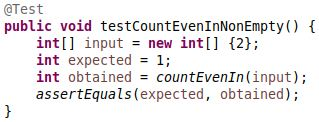
\includegraphics[width=\linewidth]{figures/stmtCoverageOrientedTests.JPG}
	\caption{Tests orientados a satisfacer cobertura de sentencias para el c\'odigo de \emph{countEvenIn(int[])} \ref{figures.code.coverageExample}.}
	\label{figures.examples.coverage.stmtTests}
\end{figure}

\begin{figure}
	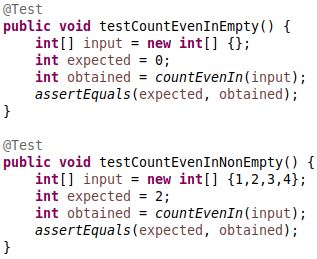
\includegraphics[width=\linewidth]{figures/branchCoverageOrientedTests.JPG}
	\caption{Tests orientados a satisfacer cobertura de ramas para el c\'odigo de \emph{countEvenIn(int[])} \ref{figures.code.coverageExample}.}
	\label{figures.examples.coverage.branchTests}
\end{figure}

\begin{figure}
	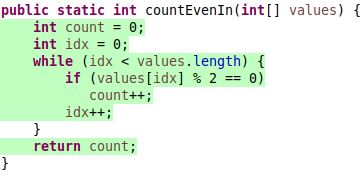
\includegraphics[width=\linewidth]{figures/branchCoverageExampleComplete.JPG}
	\caption{Medici\'on de cobertura de \emph{countEvenIn(int[])} \ref{figures.code.coverageExample} con una cobertura del 100\% tanto de sentencias como de ramas.}
	\label{figures.examples.coverage.fullCoverage}
\end{figure}

\begin{figure}
	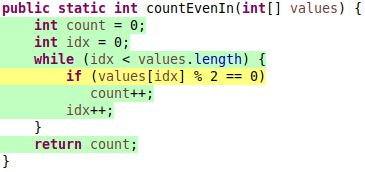
\includegraphics[width=\linewidth]{figures/branchCoverageExampleIncomplete.JPG}
	\caption{Medici\'on de cobertura de \emph{countEvenIn(int[])} \ref{figures.code.coverageExample} con una cobertura del 100\% de sentencias pero no de ramas.}
	\label{figures.examples.coverage.stmtCoverage}
\end{figure}

En el caso de criterios de caja negra, varios criterios com\'unmente utilizados se basan en analizar la especificaci\'on de las entradas esperadas por el programa a analizar. En general se comienza partiendo el dominio de cada entrada de acuerdo a ciertas caracter\'isticas provistas. \'Estas deben dividir el conjunto de valores de cada entrada en subconjuntos disjuntos, y la uni\'on de todos los subconjuntos debe resultar en el dominio completo de cada entrada. Por ejemplo, si una entrada es un entero, es posible dar como caracter\'istica a \emph{ser par}, lo que divide todo el conjunto de los enteros en dos subconjuntos disjuntos (uno conteniendo todos los enteros pares y otro conteniendo a todos los impares), tal que al unir estos conjuntos se obtiene nuevamente a todos los enteros. Cada criterio basado en las entradas del programa a evaluar define de qu\'e forma combinar valores de cada subconjunto en los casos donde el programa tiene varias entradas. Por ejemplo, combinar todos con todos, o cada subconjunto debe estar representado por lo menos una vez sin importar con qu\'e otro subconjunto es combinado. Para el ejemplo de la Figura \ref{figures.code.replaceExample}, que muestra un m\'etodo que dado un arreglo de enteros, un valor entero a buscar en el arreglo, y un valor con el cual reemplazar el valor anterior, realiza los reemplazos y retorna cuantos fueron realizados, en la Tabla \ref{tables.example.codeCoverage} se muestran posibles caracter\'isticas para dividir cada entrada: que el arreglo sea o no vac\'io; que el valor a buscar est\'e o no en el arreglo; y finalmente que el valor con el cual reemplazar al anterior sea igual o distinto al reemplazado. Vale aclarar que si bien todas las caracter\'isticas dividen las entradas en dos subconjuntos, esto no debe ser necesariamente as\'i. Una caracter\'istica que divida en m\'as subconjuntos es perfectamente v\'alida, siempre que cumpla con las propiedades mencionadas anteriormente. Como ejemplo de combinaci\'on de valores de cada subconjunto definidos por las caracter\'isticas en la Tabla \ref{tables.example.codeCoverage}, podemos utilizar el criterio \emph{Each Choice Value}, el cual determina que cada subconjunto debe estar representado al menos una vez en los tests. Esto lleva a los tests que se muestran en la Figura \ref{figures.examples.coverage.eccTests}, donde tenemos dos tests, uno donde se utiliza un arreglo no vac\'io, con el valor a reemplazar perteneciendo al arreglo (2) y el valor con el cual reemplazar siendo igual al anterior; el segundo test utiliza un arreglo vac\'io, obviamente el elemento a buscar no pertenece al mismo y el valor con el cual se realiza el reemplazo es distinto al anterior. El hecho de que como se puede apreciar en la Figura \ref{figures.examples.coverage.eccCoverage}, los tests anteriores logran una cobertura de ramas del 100\% al tiempo que \'estos son evidentemente un conjunto muy pobre de escenarios, sirve para remarcar c\'omo un criterio puede ser satisfecho al mismo tiempo que los tests que lo satisfacen son claramente de muy mala calidad.

\begin{figure}
	\lstinputlisting[basicstyle=\small, language=Java, tabsize=3]{results/draft/Replace.java}
	\caption{M\'etodo para reemplazar todos los valores en un arreglo \emph{array} que son iguales a un valor especificado (\emph{what}) por otro valor especificado (\emph{with}) y retornar cuantos cambios se realizaron.}
	\label{figures.code.replaceExample}
\end{figure}

\begin{table}[]
	\begin{tabular}{|c|ccc|}
		\hline
		Bloque & array vacío & what pertenece & with igual a what \\ \hline
		1 & T & T & T \\ \hline
		2 & F & F & F \\ \hline
	\end{tabular}
	\caption{Caracter\'isticas con las que se puede dividir los conjuntos de las entradas del programa \emph{replace(int[], int, int)} \ref{figures.code.replaceExample}.}
	\label{tables.example.codeCoverage}
\end{table}

\begin{figure}
	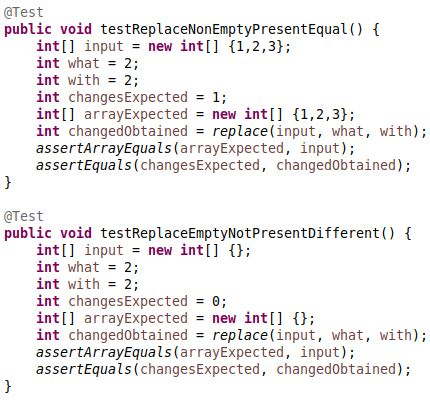
\includegraphics[width=\linewidth]{figures/replaceTestsEachChoice.JPG}
	\caption{Tests para satisfacer criterio de cobertura \emph{Each Choice Coverage} para \ref{figures.code.replaceExample} basado en las caracter\'isticas definidas en \ref{tables.example.codeCoverage}.}
	\label{figures.examples.coverage.eccTests}
\end{figure}

\begin{figure}
	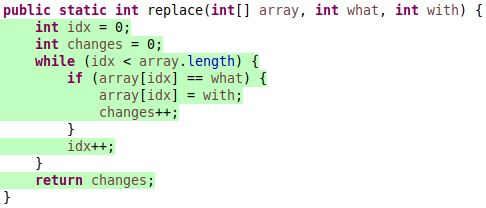
\includegraphics[width=\linewidth]{figures/replaceFullCoverage.JPG}
	\caption{Cobertura de ramas lograda por los tests definidos en \ref{figures.examples.coverage.eccTests}.}
	\label{figures.examples.coverage.eccCoverage}
\end{figure}

\chapter[Mutation]{Mutation testing}
\label{sec:preliminares.mutation}


\subsection{Evaluaci\'on de mutation testing}

Las propiedades de inter\'es en el disen\~no y evoluci\'on de operadores involucrados en mutation testing son, equivalencia de mutantes con el programa original y entre mutantes, dificultad de detecci\'on de mutantes, acoplamiento entre fallas reales y mutantes, y acoplamiento entre mutantes.

\subsubsection{Equivalencia}
Equivalencia [entre dos programas] es una propiedad definida bajo la relaci\'on \texttt{Eq(P, P$\prime$) : $\nexists$ E : P(E) != P$\prime$(E)}, la cual establece que dos programas \texttt{P} y \texttt{P$\prime$} son equivalente si no existe un escenario \texttt{E} tal que el comportamiento de ambos programas se distinto. Esta es una relaci\'on indecidible por lo que m\'etodos incompletos son utilizados. Dentro de mutation testing, equivalencia puede encontrarse entre un mutante y el programa original, un caso indeseable ya que \'estos disminuyen el valor del mutation score sin significar una deficiencia de parte del test suite en detectar ciertas fallas artificiales. Otro caso de equivalencia se da entre mutantes, un caso en donde ambos mutantes son detectados por el test suite, sin embargo al ser equivalente incrementan el valor del mutation score sin significar una mejora de parte del test suite en detectar m\'as fallas artificiales.

Dentro de la investigaci\'on sobre la detecci\'on (evaluaci\'on) de esta caracter\'istica y su impacto en el ana\'alisis de test suites usando mutation testing, \cite{biblography.mutation.evaluation.equivalent.Schuler+10} propone la utilizaci\'on de diferencia en cobertura de c\'odigo y an\'alisis de fujo de datos para determinar potencial equivalencia. Mientras que  \cite{biblography.mutation.evaluation.equivalent.Just+13} utiliza detecci\'on de restricciones condicionales para alcanzar el c\'odigo mutado y \emph{SAT Solving} para determinar si es posible satisfacer dichas restricciones al tiempo que se obtiene un valor distinto al del programa original en ese punto, lo que es similar en principio a \emph{weak mutation}, en donde se considera que un mutante es detectado si en el estado siguiente a la mutaci\'on se detecta una diferencia con el del programa original, pero a\~nadiendo control de alcanzabilidad y una verificaci\'on exhaustiva acotada para detectar si es posible que exista una diferencia.
En \cite{biblography.mutation.evaluation.equivalent.Grun+09} observan que manualmente, para los casos de estudios utilizados, un programador avanzado tarda aproximadamente 15 minutos en promedio para analizar mutantes equivalentes. Y claramente la existencia de equivalentes disminuye artificialmente el mutation score dando la falsa impresi\'on de que es necesario agregar m\'as tests.

\subsubsection{Dificultad de detecci\'on}

As\'i como los mutantes equivalentes son indeseables por ser imposibles de detectar, los mutantes que son solo detectables por un conjunto peque\~no de tests, son altamente deseables. Estos son denominados \emph{stubborn} \cite{bibliography.mutation.evaluation.stubbornHieronsHD99}. La detecci\'on de estos mutantes requieren tests de "mejor calidad" y si bien existen estudios que eval\'uan la generaci\'on de stubborns por operador \cite{bibliography.mutation.evaluation.stubborn}, \'este depende del conjunto de programas utilizados y los tests asociados. Con respecto a este obst\'aculo, en \cite{bibliography.mutation.evaluation.hardnessVisser}, proponen el uso de \emph{model counting} sobre programas m\'as simples pero utilizando un estudio m\'as exhaustivo.

\subsubsection{Subsunci\'on}

\emph{Subsumption}, la relaci\'on entre mutantes con respecto a los tests que los detectan, dan lugar a mutantes redundantes. Esto es, los tests que detectan al mutante subsumido, incluyen a aquellos que detectan al que subsume, es decir, el mutante subsumido eval\'ua de manera menos espec\'ifica a los tests ya que es detectado por una mayor cantidad, mientras que el que subsume eval\'ua tests m\'as espec\'ificos. Esto lleva a mutantes redundantes y representa una forma de evaluar la dificultad de detecci\'on, los mutantes que subsumen a otros pero no son a su vez subsumidos, son detectados por pocos tests. Presentado inicialmente en \cite{bibliography.mutation.selection.Offutt96}, mutant subsumption es utilizado por \cite{bibliography.mutation.minimizing.dynamicsubsumption} y \cite{bibliography.mutation.evaluation.JustKA17} para evaluar utilidad de mutantes dentro de mutation analysis.

\subsubsection{Acoplamiento}

\emph{Coupling}, el acoplamiento entre fallas reales y mutantes es una propiedad altamente deseable, sin la misma, mutation testing perder\'ia su utilidad al desaparecer la correlaci\'on entre un mutation score alto y una buena capacidad de parte del test suite para detectar fallas reales. El trabajo m\'as importante sobre este tema, y uno que nos representa una motivaci\'on importante para el desarrollo de nuestros operadores de mutaci\'on presentados en esta tesis, es \cite{bibliography.mutation.evaluation.valid-substitute}. El acoplamiento entre mutantes y fallas reales es una relaci\'on que especifica que si un conjunto de tests detecta un conjunto de mutantes, entonces va a detectar una falla real. 

\subsection{High order}

\texttt{High Order}, la combinaci\'on de mutaciones, generada al aplicar operadores de mutaci\'on m\'as de una vez al generar un mutante, se denominan mutaciones de alto order mientras que aquellas que la forman, se las llama de primer orden. Si bien en principio esto agregar\'ia una gran cantidad de nuevos mutantes\footnote{Usualmente la cantidad de mutantes al aplicar m\'as de una mutaci\'on por mutante est\'a acotada por M$_0^G$ en donde \texttt{M$_0$} son la cantidad de mutantes de primer orden y \texttt{G} son la cantidad de mutaciones por mutante}, los estudios actuales que se enfocan en esta t\'ecnica concluyen que estos mutantes de alto orden representan fallas artificiales m\'as sutiles y que subsumen a una gran cantidad de mutantes de primer orden. [AGREGAR]
\chapter{Mutaci\'on de expresiones de navegaci\'on en reparaci\'on de programas}
\label{cap:repair}

\section{Reparaci\'on autom\'atica de programas}
\label{sec:repair}

La aparici\'on de t\'ecnicas autom\'aticas para testing y localizaci\'on de fallas, es decir, detectar en donde puede estar una falla, una vez detectada, llev\'o a la investigaci\'on de t\'ecnicas para, una vez detectada, poder reparar dicha falla de manera autom\'atica. Pero que significa reparar una falla?
\begin{quote}
	Dado un programa \textbf{P} y una especificaci\'on \textbf{E} del mismo, si \textbf{P} no cumple con sus especificaciones (\textbf{E}), reparar al programa significa encontrar un variante \textbf{P'} mediante modificaciones sint\'acticas tal que \'esta cumpla con las especificaciones dadas por \textbf{E} \footnote{Esta definici\'on no considera reparaciones en tiempo de ejecuci\'on, es decir, aquellas que no producen una variante del programa original como reparaci\'on}.
\end{quote}
A partir del trabajo de \cite{bibliography.repair.ArcuriY08}, muchas herramientas que intentan atacar a este problema han surgido. Incluso cuando la idea de reparaci\'on autom\'atica de fallas es atractiva, reparar autom\'aticamente defectos de programas arbitrarios es inviable. Por lo tanto, la reparaci\'on autom\'atica de programas debe sacrificar completitud. Varias t\'ecnicas efectivas para reparaci\'on de programas recurren a explorar un conjunto grande (aunque limitado) de candidatos de reparaci\'on obtenidos por modificaciones sint\'acticas de un programa con fallas. Adem\'as, para que estas t\'ecnicas escalen razonzablemente, el espacio de candidatos a reparaci\'on debe ser acotado, limitando el conjunto de modificaciones sint\'acticas a considerar (por ejemplo, no considerar modificaciones a partes de una sentencia), o no explorando exhaustivamente el conjunto acotado de candidatos a reparaci\'on (por ejemplo, usando algor\'itmos gen\'eticos en lugar de b\'usqueda exhaustiva).

\subsection{Or\'aculo de reparaci\'on}
\label{sec:repair.specs}

En general el proceso de reparaci\'on sigue, a rasgos muy generales, el siguiente algoritmo:

\begin{lstlisting}[basicstyle={}, language=Java]
  repair(P, E) {
    current = P
    while (!isValid(current, E) && !boundsReached()) {
      current = nextFix();
    }
    return current;
  }
\end{lstlisting}

Donde \textbf{P} representa el programa a reparar, y \textbf{E} las especificaciones que se deben satisfacer. El proceso b\'usca candidatos a reparaciones, evaluando a \'estos con respecto a las especificaciones provistas. Claramente el proceso est\'a acotado a un conjunto finito de posibles reparaciones.

Evidentemente, es necesario definir que se usa como especificaciones para el programa. Los primeros trabajos sobre reparaci\'on autom\'atica \cite{bibliography.repair.StaberJB05, bibliography.repair.ArcuriY08}, utilizaban especificaciones formales en forma de pre y post condiciones, o descripciones l\'ogicas provistas en alg\'un formalismo l\'ogico apropiado. Sin embargo, muchas de las \'ultimas t\'ecnicas utilizan tests como especificaciones. La raz\'on principal detr\'as de esto, es el argumento de que la producci\'on de especificaciones formales es un proceso costoso, a la vez que es muy raro encontrarlas ya provistas previo al proceso de reparaci\'on, mientras que los tests son menos costosos de proveer y es mucho m\'as com\'un encontrarlos ya provistos antes del proceso de reparaci\'on.

Por ejemplo, \emph{GenProg} \cite{bibliography.repair.GouesNFW12} usa computaci\'on evolutiva para evolucionar sint\'acticamente un programa hasta que una reparaci\'on aceptable es encontrada. Cada reparaci\'on candidata (modificaci\'on sint\'actica) es aplicada al programa original para producir uno nuevo cuya aptitud es evaluada utilizando un test suite. Modificaciones sint\'acticas en partes de una sentencia no son consideradas para limitar el espacio de candidatos, y la funci\'on de aptitud es utilizada para mantener una poblaci\'on reducida de candidatos a lo largo del proceso de computaci\'on evolutiva. 

\subsubsection{Tests como especificaciones}
\label{sec:repair.specs.testsAsSpecs}

Las herramientas actuales, en general, utilizan tests como especificaciones parciales del programa a reparar. Esto tiene como consecuencia la generaci\'on de reparaciones espurias, es decir, reparaciones que si bien logran hacer ``pasar'' a los tests, no resuelven el problema. En muchos casos, enmascarar un defecto puede causar que los tests que antes detectaban una falla, ahora dejen de hacerlo. A modo de ejemplo, en la Figura~\ref{figures.examples.repair.nullaccessexample} se muestra un m\'etodo \emph{find(int)} que tiene un defecto, la condici\'on del \textbf{while} deber\'ia incluir que \textbf{current} no sea \emph{null} y que el elemento a\'un no fue encontrado. Sin embargo, la reparaci\'on en la Figura~\ref{figures.examples.repair.nullaccessexample.mask} enmascara al defecto. Si nuestros tests solo utilizan listas en donde el elemento no est\'a, y por lo tanto se espera que el m\'etodo retorne \emph{false}; o el elemento a buscar est\'a en la \'ultima posici\'on, y se espera que retorne \emph{true}. La reparaci\'on anterior es espuria, es decir, si bien logra que los tests terminen correctamente, no repara realmente el programa.

\begin{figure}
	\begin{lstlisting}[frame=single, mathescape=true,language=Java,basicstyle={},framexleftmargin=.073\textwidth,xleftmargin=.085\textwidth,xrightmargin=0.012\textwidth]
  public boolean find(int e) {
    if (isEmpty()) return false;
    Node current = header;
    boolean found = false;
    while(true) {
      found = current.elem == e;
      current = current.next;
    }
    return found;
  }
	\end{lstlisting}
	\caption[Ejemplo de bug causando \emph{NullPointerException}]{Un m\'etodo con un defecto que causa \emph{NullPointerException}}
	\label{figures.examples.repair.nullaccessexample}
\end{figure}

\begin{figure}
	\begin{lstlisting}[frame=single, mathescape=true,language=Java,basicstyle={},framexleftmargin=.073\textwidth,xleftmargin=.085\textwidth,xrightmargin=0.012\textwidth]
  public boolean find(int e) {
    if (isEmpty()) return false;
    Node current = header;
    boolean found = false;
    while(true) {
      try {
        found = current.elem == e;
        current = current.next;
      } catch (NullPointerException e) {
        break;
      }
    }
    return found;
  }
	\end{lstlisting}
	\caption{Reparaci\'on que enmascara el defecto en la Figura~\ref{figures.examples.repair.nullaccessexample}}
	\label{figures.examples.repair.nullaccessexample.mask}
\end{figure}

Esta observaci\'on llev\'o a un trabajo de investigaci\'on en donde se evaluaron un conjunto de herramientas actuales de reparaci\'on autom\'atica de programas basadas en tests como or\'aculo de reparaci\'on \cite{bibliography.repair.ZeminBGCDRAF17}. Al contrario de trabajos previos que se basaron en tests o inspecci\'on manual de las reparaciones provistas por las herramientas evaluadas (\emph{GenProg}, \emph{Angelix}, \emph{AutoFix}, y \emph{Nopol}, entre otras), en \'este, se utilizaron especificaciones formales y \emph{PEX} \cite{bibliography.formalver.TillmannH08} para evaluar las reparaciones obtenidas.

Los resultados obtenidos, logrados sobre el benchmark de reparaci\'on de programas \emph{IntroClass} \cite{bibliography.repair.benchmarks.GouesHSBDFW15}, indican que al evaluar las reparaciones producidas utilizando especificaciones formales, \'estas son inv\'alidas, es decir, el programa obtenido no cumple con las especificaciones del problema que deben resolver. El porcentaje de reparaciones para \emph{GenProg}, que son consideradas como efectivas, es solo un 1.57\% (18 de 1.143 fallas fueron reparadas) de las cuales 8 reparan errores de typos en cadenas asociadas a los mensajes de salida del programa. \emph{Angelix} solo es capaz de reparar 41 de 232 (17,67\%), \emph{Nopol} solo 6 de 297 (2\%), y finalmente \emph{AutoFix} no pudo reparar ning\'un programa de manera correcta\footnote{Algunas herramientas no soportaban ciertas caracter\'isticas (retornar una cadena), y en otras que requer\'ian traducir a otro lenguaje, la misma reparaba el defecto}. Por el otro lado, incrementar la cantidad de tests disminu\'ia dr\'asticamente las reparaciones espurias, pero tambi\'en las reparaciones en general. En otros casos, las herramientas no soportaban el aumento en la cantidad de tests.

\subsection{Granularidad de las reparaciones}
\label{sec:repair.granularity}

Como mencionamos anteriormente, el conjunto de candidatos a reparaci\'on a tener en cuenta, debe ser finito y su tama\~no afecta directamente a los recursos necesarios para reparar el programa. Esto genera una necesidad de balancear capacidad de reparaci\'on, es decir, que tipo de fallas se pueden reparar, con recursos necesarios. Por ejemplo, el caso de \emph{GenProg}, se basa en mover, duplicar, o eliminar c\'odigo. La idea es que muchas veces un desarrollador escribe varias veces el mismo c\'odigo, por ejemplo, sumarle 1 a una variable. Por otro lado, en \emph{SPR} \cite{bibliography.repair.LongR15}, se generan reparaci\'ones abstractas como agregar una condici\'on \textbf{C} antes de la ejecuci\'on de una sentencia, la cual luego ser\'a reemplazada por una condici\'on concreta en una etapa posterior, esto sumado a la eliminaci\'on, y duplicaci\'on de c\'odigo existente. En \emph{PAR} \cite{bibliography.repair.KimNSK13}, las modificaciones para reparar el programa son aprendidas a partir de patrones en reparaciones escritas manualmente. Por esto, el n\'umero de candidatos a considerar como reparaciones es significativamente reducido, lo que a su vez reduce el tipo de errores que la t\'ecnica puede ser capaz de reparar.

Modificaciones a partes de sentencias, es decir, aquellas que alteran expresiones dentro de una sentencia, son en general no consideradas por t\'ecnicas de reparaci\'on de programas. Una limitaci\'on principal al considerar a \'estas, es la explosi\'on en el espacio de candidatos de reparaci\'on. T\'ecnicas que utilizan operadores de mutaci\'on para producir las modificaciones sint\'acticas, y que incluyen modificaciones a partes de sentencias, requieren limitar el conjunto de mutaciones (por ejemplo, \cite{bibliography.repair.GopinathMK11}), reduciendo la clase de fallas que \'estas pueden intentar reparar.

\begin{figure}
\footnotesize
\begin{lstlisting}[frame=single, mathescape=true,language=Java,basicstyle={},xleftmargin=.010\textwidth,xrightmargin=.007\textwidth]
boolean add(Object arg) {
  SListNode freshNode = new SListNode();
  freshNode.value = arg;
  boolean added = false;
  if (this.header == null) {
    this.header = freshNode;
    added = true;
  } else {
    SListNode current = this.header.next; //BUG: ignora primer nodo
    while (current.next ! = null && current.value ! = arg) {
      current = current.next;
    }
    if (current.value ! = arg) {
      current.next = freshNode;
      added = true;
    }
  }
  if (added) {
    size = size - 1; //BUG: decrementa size
  }
  return added;
}
\end{lstlisting}
\caption[Programa con dos bugs intra-sentencia]{Ejemplo de c\'odigo con dos bugs que requieren modificaciones intra-sentencia}
\label{figures.examples.repair.exampleCode}
\end{figure}

Los efectos que tienen estas restricciones sobre el espacio de candidatos a considerar para la reparaci\'on, pueden observarse en la Figura~\ref{figures.examples.repair.exampleCode} donde se muestra el m\'etodo \emph{add(Object)} de un conjunto. \'Este contiene dos defectos: primero, cuando el conjunto no est\'a vaci\'o, se comienza el recorrido del mismo a partir del nodo siguiente al inicial (el cual podr\'ia ser \emph{null}, resultando en un error en la l\'inea siguiente); segundo, cuando un nuevo nodo es agregado a la lista sobre la cual est\'a implementado el conjunto, el tama\~no de la misma (atributo \emph{size}) se decrementa. Para reparar al m\'etodo es necesario realizar dos cambios, ambos dentro de una sentencia. En herramientas que hacen cambios a nivel bloque, solo es posible reparar el programa si existen en otro punto del c\'odigo las sentencias \textbf{current = this.header;} y \textbf{size = size + 1}.


\subsubsection{Mutaci\'on en reparaci\'on}
\label{sec:repair.granularity.mutation}

El uso de operadores de mutaci\'on, provenientes de mutation testing, en reparaci\'on de programas, parece razonable: si estos operadores son utilizados en mutation testing para emular defectos reales, podr\'ian utilizarse para emular reparaciones. Ejemplos recientes de herramientas de reparaci\'on autom\'atica de programas son \cite{bibliography.repair.mutation.DebroyW10} y  \cite{bibliography.repair.mutation.AlloyWang18}. El argumento de utilizar mutaci\'on en reparaci\'on de programas es que existen mutaciones que si se fueran a combinar, se cancelar\'ian, por ejemplo:
\begin{lstlisting}[mathescape=true, language=Java,basicstyle={}]
  for (int i = 0; i < lenght; i++)...
  $\Delta$for (int i = 0; i > lenght; i++)...
\end{lstlisting}
donde la primera sentencia se puede mutar, aplicando un cambio de operador relacional, a la segunda, marcada por $\Delta$, que a su vez se puede mutar al c\'odigo original aplicando el mismo operador de mutaci\'on. Aunque no siempre se puede deshacer una mutaci\'on aplicando otra que sea sint\'acticamente inversa. 
Volviendo al ejemplo anterior, el mutante:
\begin{lstlisting}[mathescape=true, language=Java,basicstyle={}]
  for (int i = 0; i > lenght; i++)...
\end{lstlisting}
puede ser restaurado, sem\'anticamente, generando el mutante:
\begin{lstlisting}[mathescape=true, language=Java,basicstyle={}]
  for (int i = 0; i $\textbf{!=}$ lenght; i++)...
\end{lstlisting}
Existen tambi\'en casos donde varias mutaciones pueden corregir el comportamiento. Esto lleva a la idea de que si consideramos el programa con fallas \texttt{P$_b$} y el original sin fallas \texttt{P$_o$}, se puede definir el segundo en t\'erminos del primero como \texttt{P$_b$ = mutate(P$_o$, M)} donde \texttt{M} representa una secuencia de mutaciones y \texttt{mutate} es un programa que aplica dicha secuencia a un programa. En general como dijimos anteriormente, muchas mutaciones tienen su inversa, ya sea sint\'actica o sem\'antica, lo que lleva a definir el problema de reparaci\'on como encontrar una secuencia de mutaciones \texttt{M$\prime$} tal que \texttt{P$_o$ = mutate(P$_b$, M$\prime$)}.

La reparaci\'on de programas puede describirse como una b\'usqueda exhaustiva que, dado un programa defectuoso y una especificaci\'on del mismo (que como vimos puede ser formal o mediante tests), y un conjunto de operadores de mutaci\'on:
\begin{enumerate}
	\item Considera el programa a reparar como el candidato a reparaci\'on inicial.
	
	\item Si \textbf{P} es un candidato a reparaci\'on, y \textbf{Q} es el resultado de aplicar una mutaci\'on a \textbf{P}, entonces \textbf{Q} tambi\'en es un candidato a reparaci\'on.
	
	\item  Un candidato \textbf{S} es exitoso si satisface las especificaciones provistas.
\end{enumerate}

\begin{figure}
	\centering
	\begin{tikzpicture}%
	[state/.style ={ellipse, draw, minimum width = 0.7 cm},
	point/.style = {circle, draw, inner sep=0.04cm,fill,node contents={}},
	el/.style = {inner sep=2pt, align=left, sloped}]
	\node[state,rectangle] (init) {$return\:a < b?a:b;$};
	\node[state,rectangle] (cand1) [below=of init] {$return\:b < b?a:b;$};
	\node[state,rectangle] (cand2) [right=of cand1] {$return\:a < b?a:0;$};
	\node[state,rectangle] (succ) [below=of cand1] {$return\:b < a?a:b;$};
	
	\path[->] (init) edge node[left] {a -> b} (cand1);
	\path[->] (init) edge node[right=16pt] {b -> 0} (cand2);
	\path[->] (cand1) edge node[left] {b -> a} (succ);
	
	\node[label=right: {\small Inicial}, draw=blue,dotted,fit=(init)] (initR) {};
	
	\node[label=right: {\small Candidatos (Profundidad 1)},draw=blue,dotted,fit=(cand1) (cand2), inner sep=0.2cm] (Candidates) {};
	
	\node[label=right: {\small Exitoso (Profundidad 2)},draw=blue,dotted,fit=(succ)] (Succ) {};
	
	\end{tikzpicture}
	\caption[Reparaci\'on como b\'usqueda, ejemplo]{Reparaci\'on de un programa que calcula el m\'aximo de dos n\'umeros}
	\label{figures.examples.repairWithMutation}
\end{figure}

La definici\'on previa de reparaci\'on autom\'atica de programas deja en claro que el espacio de candidatos a reparaci\'on depende del n\'umero de mutaciones (\textbf{b}) a considerar, lo que influye en cuan ``ancho'' es el \'arbol de b\'usqueda, y el n\'umero m\'aximo de mutaciones sucesivas permitidas (\textbf{d}) para generar a los candidatos, lo que afecta la profundidad de la b\'usqueda. El espacio de b\'usqueda queda entonces definido por una suma geom\'etrica $\frac{b^{d+1}-1}{b-1}$ ($O(b^d)$). Si consideramos el m\'etodo en la Figura~\ref{figures.examples.repair.getNode}, y solo cuatro l\'ineas del mismo, al utilizar 18 operadores de mutaci\'on (mediante la herramienta \emph{$\mu$Java++}), podemos ver en la Tabla \ref{tables.repair.mutation.explosion}, como a medida que aumentamos la cantidad de mutaciones consecutivas (la profundidad en reparaci\'on mediante mutaci\'on), la cantidad de candidatos a evaluar se vuelve r\'apidamente inmanejable.

\begin{figure}
	\begin{lstlisting}[frame=single, mathescape=true,language=Java,basicstyle={},framexleftmargin=.073\textwidth,xleftmargin=.085\textwidth,xrightmargin=0.012\textwidth]
  Node getNode(int i) {
    Node current = this.head;
    Node result = null;
    int current_index = 0;
    while (result == null && current != null) {
      if (i == current_index ) {
        result = current;
      }
      current_index = current_index + 1;
      current = current.next;
    }
    return result;
  }
	\end{lstlisting}
	\caption[M\'etodo de ejemplo, \emph{getNode(int)}]{C\'odigo de ejemplo, m\'etodo que obtiene el i-\'esimo nodo de una lista}
	\label{figures.examples.repair.getNode}
\end{figure}

\begin{table}[t]
	\caption[Mutantes para \emph{getNode} (Figura~\ref{figures.examples.repair.getNode}) a diferentes profundidades]{Mutantes generados para \emph{getNode} de la Figura~\ref{figures.examples.repair.getNode}, considerando 4 l\'ineas y 18 operadores, a medida que la profundidad aumenta.}
	\label{tables.repair.mutation.explosion}
	\begin{center}
		\small
		\begin{tabular}{c r}
			Search Depth                            &	No. of Mutants (Fix Candidates)        \\
			\hline
			1 					&	40		                               	\\
			2 					&	1,604			                \\
			3 					&	64,684		        	        \\
			4 					&	$>$ 20 million		                
		\end{tabular}
		\normalsize
	\end{center}
\end{table}

\pagebreak
\subsection{Striker}
\label{sec:repair.striker}

\emph{Striker} es una herramienta de reparaci\'on autom\'atica de programas cuya meta principal es:
\begin{quote}
	Proveer una t\'ecnica automatizada y eficiente para reparar programas anotados con especificaciones (en t\'erminos de pre y post condiciones) corrigiendo errores que resultan como una consecuencia de ocurrencias simultaneas de un n\'umero de errores sint\'acticos dentro de sentencias de un programa.
\end{quote}
Es necesario remarcar la necesidad de especificaciones asociadas al programa. As\'i tambi\'en, los errores que se consideran son defectos, o mutaciones, dentro de sentencias. En particular no se apunta a reparar programas que requieran agregar, o eliminar, c\'odigo. Algunos de los defectos reparables por \emph{Striker} se muestran en la Figura~\ref{figures.examples.repair.faultsGetNode}.

Si bien muchas herramientas de reparaci\'on autom\'atica de programas utilizan mutaci\'on, \emph{Striker} es una de las m\'as flexibles con respecto a operadores soportados, entre ellos \emph{PRVO}; soporte para modificaciones a partes de sentencias; y fallas que requieren las modificaci\'on de varias sentencias. Striker utiliza \emph{TACO} \cite{bibliography.mutation.tools.TACOGaleottiRPF13} para evaluar candidatos a reparaci\'on, lo que requiere proveer especificaciones formales en lugar de un test suite, y JML RAC \cite{bibliography.misc.JMLRAC.LeavensCCRC02} como t\'ecnica de evaluaci\'on r\'apida basada en escenarios previamente encontrados para los cuales un candidato a reparaci\'on no cumpl\'ia con las especificaciones. Sin entrar en detalles, esta herramienta es capaz de expandir las fallas soportadas para reparar, agregando varios operadores en los que se incluye a \emph{PRVO}, y permitir la reparaci\'on de aquellas que requieren modificaciones intra-sentencias as\'i como en m\'ultiples sentencias, mediante el uso de t\'ecnicas de poda innovadoras.

Bajo esta herramienta es que se pudo observar como \emph{PRVO} era capaz de reparar ciertas fallas que de otra forma no eran reparables, como por ejemplo el caso de \emph{add(int)} en la Figura~\ref{figures.examples.repair.exampleCode}, en donde si bien el segundo defecto es reparable por \emph{AORB} el cual reemplaza el operador incorrecto (\emph{-}) por el que corresponde (\emph{+}), el primer defecto solo puede ser reparado por \emph{PRVO} al eliminar el acceso al campo \emph{next}. Si bien el enfoque principal de esta tesis se encuentra en \emph{PRVO} como un operador de mutaci\'on en el contexto de mutation testing, es interesante mostrar su contribuci\'on en el contexto de reparaci\'on.

\begin{figure}[t]
	\footnotesize
	$$
	\begin{array}{rl}
	5_a: & (\mathit{result} \mbox{ != }\mathsf{null}\ \&\&\ \mathit{current}\mbox{ != }\mathsf{null})\\
	5_b: & (\mathit{result} == \mathsf{null}\ \&\&\ \mathit{current} == \mathsf{null})\\
	5_c: & (\mathit{result} == \mathsf{null}\ ||\ \mathit{current}\mbox{ != }\mathsf{null})\\
	6_a: & (\mathit{i} == \mathit{current\_index} + 1)\\
	6_b: & (\mathit{i}\ \mbox{!=}\ \mathit{current\_index})\\
	9_a: & \mathit{current\_index} = \mathit{current\_index} - 1\\
	10_a: & \mathit{current.next} = \mathit{current}
	\end{array}
	$$
	\normalsize
	\caption[Defectos del algoritmo en la Figura~\ref{figures.examples.repair.getNode} reparables por \emph{PRVO}]{Algunos defectos en el m\'etodo \emph{getNode} de la Figura~\ref{figures.examples.repair.getNode} que pueden modelarse mediante mutaciones y ser reparados por \emph{PRVO}.}
	\label{figures.examples.repair.faultsGetNode}
\end{figure}

\subsection{Evaluaci\'on de Stryker}
\label{sec:repair.striker.evaluation}

Si bien la evaluaci\'on de \emph{Stryker} se encuentra enfocada hacia la t\'ecnica de poda del espacio de b\'usqueda de candidatos a reparaci\'on, lo que a su vez permite la utilizaci\'on de una mayor cantidad de operadores de mutaci\'on orientados hacia la reparaci\'on de fallas intra-sentencia, en el contexto de esta tesis nos interesan los resultados asociados a \emph{PRVO} y su utilidad en el campo de reparaci\'on autom\'atica de programas mediante operadores de mutaci\'on utilizados en mutation testing, los cuales son m\'as granulares en el tipo de cambios que realizan lo que permite incrementar la reparabilidad de programas.

En los experimentos realizados para la evaluaci\'on de \emph{Stryker}, se utilizaron implementaciones en \emph{Java} de estructuras que representan colecciones. Estas clases, para las cuales se definieron especificaciones en forma de contratos \emph{JML}, incluyendo clausulas \texttt{requires/ensures}, funciones de variantes de ciclos e invariantes de clases, son las siguientes:
\begin{itemize}
	\item \textbf{SinglyLinkedList :} Una implementaci\'on de listas simplemente encadenadas. Donde consideramos un m\'etodo \emph{contains} para evaluar pertenencia, \emph{getNode} para obtener el i-\'esimo elemento en la lista, y el m\'etodo \emph{insert} para agregar un nuevo elemento a la lista.
	
	\item \textbf{NodeCachingLinkedList :} Una lista circular, doblemente encadenada y con una cache de nodos. Considerando los m\'etodos \emph{contains}, \emph{inserte}, y \emph{remove}. Siendo el \'ultimo de particular inter\'es por almacenar nodos removidos en la cache.
	
	\item \textbf{BinarySearchTree :} Una implementaci\'on de un \'arbol de b\'usqueda binario con los m\'etodos \emph{contains}, \emph{insert} y \emph{remove}.
	
	\item \textbf{BinomialHeap :} Una implementaci\'on de colas de prioridad utilizando \emph{binomial heaps}. Considerando los m\'etodos \emph{findMin} (para obtener el m\'inimo elemento almacenado), \emph{insert}, y \emph{extractMin} para obtener y eliminar el m\'inimo elemento almacenado.
\end{itemize}

Los casos de estudio para reparaci\'on fueron obtenidos a partir de las versiones originales (correctamente implementadas) al insertar hasta $4$ mutaciones por m\'etodo, y luego se eligieron 5 versiones al azar por cada n\'umero de mutaciones insertadas, es decir, 5 programas incorrectos con un bug, 5 con 2, y as\'i hasta $4$ bugs.

Por cada sentencia (o l\'inea) mutada se agrego un comentario de l\'inea \texttt{//mutGenLimit K} donde \texttt{K} corresponde a la cantidad de bugs artificiales introducidos en la misma. Algunos ejemplos de los casos de estudios utilizados se muestran a continuaci\'on.

\begin{figure}[H]
	\lstinputlisting[basicstyle=\footnotesize, language=Java, tabsize=1,literate={\ \ }{{\ }}1]{results/repair/BinomialHeap_extractMin_orig.java}
	\caption[\emph{BinomialHeap\#extractMin}, original con contratos]{Versi\'on original del m\'etodo \emph{extractMin} de \emph{BinomialHeap} con los contratos asociados al m\'etodo.}
	\label{figures.code.repair.binheap_extractMin_orig}
\end{figure}

\begin{figure}[H]
	\lstinputlisting[basicstyle=\footnotesize, language=Java, tabsize=1,literate={\ \ }{{\ }}1]{results/repair/BinomialHeap_extractMin_4bugs.java}
	\caption[\emph{BinomialHeap\#extractMin}, $4$ bugs]{Versi\'on con $4$ bugs artificiales del m\'etodo \emph{extractMin} de \emph{BinomialHeap}.}
	\label{figures.code.repair.binheap_extractMin_4bugs}
\end{figure}

\begin{figure}[H]
	\lstinputlisting[basicstyle=\footnotesize, language=Java, tabsize=1,literate={\ \ }{{\ }}1]{results/repair/BinTree_insert_orig.java}
	\caption[\emph{BinarySearchTree\#insert}, original con contratos]{Versi\'on original del m\'etodo \emph{insert} de \emph{BinarySearchTree} con los contratos asociados al m\'etodo.}
	\label{figures.code.repair.bintree_insert_orig}
\end{figure}

\begin{figure}[H]
	\lstinputlisting[basicstyle=\footnotesize, language=Java, tabsize=1,literate={\ \ }{{\ }}1]{results/repair/BinTree_insert_3bugs.java}
	\caption[\emph{BinarySearchTree\#insert}, $3$ bugs]{Versi\'on con $3$ bugs artificiales del m\'etodo \emph{insert} de \emph{BinarySearchTree}.}
	\label{figures.code.repair.bintree_insert_3bugs}
\end{figure}

\begin{figure}[H]
	\lstinputlisting[basicstyle=\footnotesize, language=Java, tabsize=1,literate={\ \ }{{\ }}1]{results/repair/NCLL_contains_orig.java}
	\caption[\emph{NodeCachingLinkedList\#contains}, original con contratos]{Versi\'on original del m\'etodo \emph{contains} de \emph{NodeCachingLinkedList} con los contratos asociados al m\'etodo.}
	\label{figures.code.repair.ncll_contains_orig}
\end{figure}

\begin{figure}[H]
	\lstinputlisting[basicstyle=\footnotesize, language=Java, tabsize=1,literate={\ \ }{{\ }}1]{results/repair/NCLL_contains_4bugs.java}
	\caption[\emph{NodeCachingLinkedList\#contains}, $4$ bugs]{Versi\'on con $4$ bugs artificiales del m\'etodo \emph{contains} de \emph{NodeCachingLinkedList}.}
	\label{figures.code.repair.ncll_contains_4bugs}
\end{figure}

Cuando las sentencias marcadas para reparar (anotaci\'on \texttt{//mutGenLimit K}) resultaron ser un superconjunto de las sentencias con defectos, \emph{Stryker} fue capaz de reparar hasta $4$ bugs. En caso contrario \emph{Stryker} fue capaz de limitar considerablemente el espacio de b\'usqueda explorado.

%\include{requisitos-software}

\part{Generando mutaciones para expresiones de navegaci\'on} \ctparttext{text}
\cleardoublepage\null
%!TEX root = main.tex
\chapter[PRVO]{PRVO una familia de operadores para expresiones de navegaci\'on}
\label{sec:prvo}

\section{Expresiones de navegaci\'on}
\label{sec:prvo.navigationalExpressions}

Para definir nuestra familia de operadores, primero necesitamos definir que consideramos como una \emph{expresi\'on encadenada}. Una expresi\'on encadenada involucra un \emph{operador de navegaci\'on}. En Lenguajes orientados a objetos, el operador de navefaci\'on puede tomar distintas formas sint\'acticas, con la notaci\'on punto siendo la encontrada com\'unmente. Su prop\'osito es acceder a miembros de una instancia de clase. Por simplicidad nos referiremos a una expresi\'on encadenada a una que cuenta con cero o m\'as de estos operadores. El tama\~no de una expresi\'on encadenada est\'a dada por el n\'umero de operadores de navegaci\'on involucrados. Una \emph{expresi\'on de navegaci\'on} es una expresi\'on encadenada de tama\~no 1 o m\'as.

En una expresi\'on encadenada, el tipo de la misma est\'a dado por la \'ultima expresi\'on en la cadena. Por ejemplo \lstinline|a.b.c| es una expresi\'on encadenada de tama\~no tres cuyo tipo est\'a dado por el de \emph{c}. Una expresi\'on de navegaci\'on bien tipada se puede definir de dos formas. Por pertenencia, para toda cadena \texttt{a.b}, \texttt{b} es un miembro de la clase de \texttt{a}. Si cada tipo representa un conjunto y los miembros de una clase representan relaciones entre instancias de un tipo en instancias de otro (no necesariamente distintos), entonces es posible generar un grafo con las las posibles expresiones encadenadas v\'alidas.
[AGREGAR IMAGENES/GRAFICOS]

\section{PRVO}
\label{sec:prvo.prvo}
%DEFINIR OPERADORES DE PRVO COMO CONFIGURACIONES PARECE INTERESANTE

Todas las mutaciones que van a ser generadas est\'an centradas en expresiones encadenadas, que como definimos anteriormente, son aquellas expresiones que involucran cero o m\'as operadores de navegaci\'on, el punto en el caso de \emph{Java}. Esto significa que mutar una variable por otra es una posible mutaci\'on. En \emph{$\mu$Java}, un operador as\'i ya existe, llamado \emph{PRV} \cite{bibliography.mutation.operators.MaKO02}. En \emph{$\mu$Java++} este operador est\'a incluido en nuestra familia de operadores. Teniendo en cuenta que \'este operador ya es capaz de generar una cantidad significativa de mutaciones y pretendemos agregar mutaciones a mayor cantidad de expresiones, lleva a la necesidad de definir una familia de operadores. De todas formas, es posible dar definici\'on general de \emph{prvo} de la siguiente manera:
\begin{quote}
	Dada una expresi\'on encadenada $e$, \emph{prvo} va a generar mutaciones al reemplazar sub-expresiones en $e$, respectando el tipo de la expresi\'on, y manteniendo, incrementando, o decrementando su tama\~no.
\end{quote}
La Figura-\ref{figures.definitions.prvo.simple_def} define a la familia de operadores, como una gram\'atica. Como un ejemplo simple de mutaciones de \emph{prvo}, consideremos la expresi\'on \texttt{front}; las mutaciones generadas incluyen \texttt{front.next}, \texttt{null}, \texttt{front.next.next}, \texttt{front.next.elem}, \texttt{front.next.next.next}, entre otras. Un claro problema con la definici\'on anterior es que es recursiva y no acodata, en el sentido de que no hay un l\'imite sobre cuanto puede incrementarse o decrementarse el tama\~no de una expresi\'on.

\begin{figure}
	\begin{displaymath}
	\begin{array}{lll}
	PRVO(x)		& :=	& expression \\
	& := & PRVO(x).expression \\
	& := & expression.PRVO(x) \\
	\\
	PRVO(x.y)	& :=	& expression^{*} \\
	& :=	& PRVO(x).expression \\
	& :=	& expression.PRVO(y) \\
	& :=	& PRVO(x).expression.PRVO(y) \\
	& :=	& expression.PRVO(x).PRVO(y) \\
	& :=	& PRVO(x).PRVO(y).expression \\
	\\
	
	\multicolumn{3}{l}{\tiny{^{*} \: : \: puede \: incluir \: x \: or \: y}} \\
	\multicolumn{3}{l}{\tiny{expresi\'on \: : \: llamada \: a \: m\'etodo \: , \: acceso \: a \: atributo \: , variable \: \'o \: literal}}
	\end{array}
	\end{displaymath}
	\caption{Definici\'on abstracta de \emph{prvo}}
	\label{figures.definitions.prvo.simple_def}
\end{figure}

La definci\'on general de \emph{prvo} es muy similar a la de un generador de sentencias que pertenecen a una gram\'atica. Donde los t\'ipos definen a la misma. Si hubiera un programa definido mediante expresiones encadenadas y tipos, en donde encontrar\'iamos expresiones como \lstinline|if(a.gt().b).then(result.assign(a)).else(result.assign(b)).return(result)|, \emph{prvo} podr\'ia generar cualquier programa correcto desde un punto de vista de tipos. Principalmente por que las expresiones que puede utilizar no est\'an restringidas en absoluto. Esta caracter\'istica hace que \emph{prvo} sea completamente inservible para mutation testing. Lo que obliga a establecer restricciones, esto sin embargo, es una caracter\'istica positiva de \emph{prvo}, ya que cualquier operador en la familia de operadores \emph{prvo}, es en realidad una configuraci\'on particular de la misma. Lo que nos permite definir operadores a medida y aumentar la eficiencia de los mismos para cada caso.

Para mostrar esto pasemos a un ejemplo simple. Teniendo en cuenta los criterios para el disen\~no de operadores de mutaci\'on, discutidos en [REFERENCIA], en particular con respecto al n\'umero de mutaciones que un operador produce, es necesario proveer algunas cotas razonables para la aplicaci\'on de \emph{prvo}. El n\'umero de mutantes generados por \emph{prvo} puede ser limitado al limitar tres caracter\'isticas: las expresiones \emph{objetivo} (donde se va a aplicar \emph{prvo}); el \emph{tama\~no de las expresiones}, por cuanto se permite cambiar, incrementar o reducir, el tama\~no de las expresiones resultantes (las mutaciones); y los \emph{reemplazos}, es decir, las expresiones que se van a usar para el intercalado/substituci\'on en \emph{prvo}. En cuanto a los objetivos, \emph{prvo} solo va a ser aplicado a expresiones de navegaci\'on, es decir, expresiones que involucran al menos una navegaci\'on. Respecto al tama\~no, vamos a limitar \emph{prvo} a producir expresiones del \emph{mismo} tama\~no que la expresi\'on original (el n\'umero de navegaciones se mantiene). En cuanto a los reemplazos, solo vamos a reemplazar expresiones con otras de exactamente el mismo tipo (al contrario de considerar definiciones menos estrictas, que permitir\'ian utilizar tipos compatibles m\'as generales), que pertenezcan a la misma clase en donde se encuentra la expresi\'on original, o en clases directamente alcanzables desde esta clase.

Hemos definido un operador de \emph{prvo} como una serie de restricciones a la definici\'on abstracta/general. Esto nos permite centrarnos en cierto tipo de fallas particulares sin perder la habilidad de eventualmente generar otra configuraci\'on que se centra en otras.

\section{Fallas asociadas a PRVO}

En \cite{bibliography.mutation.evaluation.valid-substitute} se concluyen que cierto tipo de fallas reales requieren mejorar o definir operadores de mutaci\'on para representarlas. Mientras que cierto tipo de fallas reales se consideran como imposibles de acoplar a mutantes. En esta tesis estamos interesados en aquellas fallas que pueden ser acopladas a \emph{prvo}, aun cuando algunas de estas solo puedan ser parcialmente acopladas, en referencia a que solo un subconjunto de las mismas pueden representarse mediante \emph{prvo}. En cuanto a las fallas que nos interesan, es necesario especificarlas bien y analizar como deber\'iamos configurar un ``operador'' en \emph{prvo}, la palabra \emph{operador} no se puede asociar directamente con un conjunto de funciones como ocurre en la pr\'actica, sin\'o que se refiere a una configuraci\'on particular de estas funciones. %LA ULTIMA PARTE YA FUE MENCIONADA

\subsection{Fallas que requieren mejorar operadores existentes}

\subsubsection{Eliminaci\'on de sentencias}

Una sentencia olvidada, donde un ejemplo simple es la implementaci\'on de un ciclo infinito con una sentencia de retorno bajo cierta condici\'on [FIGURA]; una sentencia \emph{switch} en donde para alg\'un caso no se escribi\'o una sentencia de retorno o frenado (\emph{break}); nicializaciones faltantes, entre otros casos, son todos ejemplos de fallas reales que requieren un operador que elimine sentencias para poder generar el mismo tipo de falla.

En principio, ya existen operadores que realizan este tipo de mutaciones. No solo eso, sino que adem\'as no parece ser un tipo de fallas asociada mutaciones de expresiones encadenadas.

Sin embargo, \emph{Fluent interfaces}, un disen\~o muy usado en conjunto con \emph{patr\'on Builder}, permite escribir algoritmos sem\'anticamente equivalentes a un programa imperativo, ciclos y sentencias condicionales inclu\'idas. Un c\'odigo como \lstinline|list.foreach().filter(c1).if(c2).then(p1).else(p2)| no es extra\~no en programaci\'on orientada a objetos, en la Figura-\ref{figures.examples.fluent.example1.imperative} se muestra la implementaci\'on m\'as com\'un de esta expresi\'on en lenguaje imperativo.

\begin{figure}
	\begin{lstlisting}[frame=single, mathescape=true,framexleftmargin=1.5em]
  List<Elem> list = ...;
  for (Elem e : list) {
    if (c1(e)) {
      if (c2(e)) {
        p1(e);
      } else {
        p2(e);
      }
    }
  }
	\end{lstlisting}
	\label{figures.examples.fluent.example1.imperative}
	\caption{Versi\'on en lenguaje imperativo del recorrido de una lista filtrando y ejecutando condicionalmente un procedimiento.}
\end{figure}

Esto muestra que por un lado es interesante poder mutar expresiones de navegaci\'on de este tipo. Adem\'as, uno de los principales problemas con operadores que eliminan o insertan sentencias, es que suelen generar numerosos mutantes triviales que son detectados por no compilar o por que se elimin\'o directamente una gran parte de c\'odigo por una sentencia de control faltante. En \emph{interfaces fluentes}, el uso de jerarqu\'ia de tipos para garantizar la correctitud de una expresi\'on garantiza que nunca va a ser posible eliminar una sentencia cuando \'esta es necesaria.

\subsubsection{Intercambio de argumentos}

Este tipo de fallas involucra utilizar argumentos con tipos correctos, pero en el orden incorrecto en la llamada a un m\'etodo. En la Figura-\ref{figures.examples.argumentSwap.example1} se ve un m\'etodo que toma como entrada dos listas y agrega la primera al final de la segunda. Los nombres de los argumentos son quiz\'as amb\'ig\"{u}os, y ser\'ia incluso esperable que sin una documentaci\'on apropiada, haya programadores que asuman que se hace un \emph{append} de \texttt{thiz} \emph{en} \texttt{that}, aunque otros podr\'ian entender de que el \emph{append} se hace con el orden de los argumentos resultando en \texttt{that} \emph{en} \texttt{thiz}. 

\begin{figure}
	\begin{lstlisting}[frame=single, mathescape=true,framexleftmargin=1.5em]
	public void append(List<E> thiz, List<E> that) {
		...
		for (E e : thiz) {
			that.append(e);
		}
	}
	\end{lstlisting}
	\label{figures.examples.argumentSwap.example1}
	\caption{M\'etodo que agrega una lista al final de otra.}
\end{figure}

Este tipo de fallas es equivalente a aplicar dos mutaciones de cambio de referencias, \lstinline|append(thiz,that) -> append(that,that) -> append(that,thiz)|. Un tipo de mutaci\'on de expresiones de cadena de tama\~no 1, salvo que requiere dos cambios en una misma mutaci\'on. Este tipo de mutaciones no puede definirse como una serie de restricciones a la definici\'on de \emph{prvo} ya que incluye definiciones extra para incluir m\'ultiples cambios. Sin embargo vale la pena notar que con dos mutaciones de \emph{prvo} podr\'ia lograrse.

\subsubsection{Llamada a un m\'etodo similar de la misma librer\'ia}

Existen ejemplos de m\'etodos que si bien distintos, tienen una sem\'antica relacionada, \texttt{indexOf} y \texttt{lastIndexOf} son dos m\'etodos de la clase \emph{java.lang.String} que permiten obtener el primer \'indice de ocurrencia de una subcadena, o el \'ultimo respectivamente. Un operador que modifique una llamada a un m\'etodo por todas las posibles, generar\'ia una cantidad demasiado grande de mutantes para ser \'util. Sin embargo cometer una equivocaci\'on al usar un m\'etodo por otro con una sem\'antica similar, es com\'un. Este es un caso de un tipo de fallas que se pueden generar utilizando restricciones sobre \emph{prvo}.

\subsection{Fallas que requieren nuevos operadores}

\subsubsection{Omitir la llamada a un m\'etodo}

Retomemos el ejemplo de \emph{interfaces fluentes}, \lstinline|list.foreach().filter(c1).if(c2).then(p1).else(p2)|. Si en este c\'odigo nos olvid\'aramos de llamar \texttt{filter(c1)}, la expresi\'on seguir\'ia siendo correcta solamente que aplicar\'iamos el tratamiento condicional a todos los elementos de la lista en lugar de solo a aquellos que filtrar\'ia \texttt{c1}. Un ejemplo m\'as sencillo, una aplicaci\'on que toma un valor dado por el usuario y realiza una consulta en una base de datos. Es un caso t\'ipico de uso de datos no confiables, lo normal es limpiar o validar los datos ingresados antes de hacer la consulta. Una posible implementaci\'on ser\'ia:
\begin{lstlisting}
  ...
  String userQuery = getFromUser();
  List<Result> results = database.execute(cleanQuery(query));
  ...
\end{lstlisting}
Un error cl\'asico ser\'ia que el desarrollador olvide de usar \texttt{cleanQuery(query)} y directamente use \texttt{query}. Ambos casos responden a configuraciones particulares de \emph{prvo}. El primer caso, restringir las expresiones objetivo a llamadas a m\'etodos involucradas en una expresi\'on de navegaci\'on. El segundo caso responde a restringir las expresiones objetivo a llamadas a m\'etodos en casos donde \'esta ocurra en una condici\'on, argumento u asignaci\'on, siempre que el tipo de retorno del m\'etodo sea igual o compatible con el del argumento usado en la llamada. Para los ejemplos anterior se obtendr\'ian los mutantes \lstinline|list.foreach().if(c2).then(p1).else(p2)| y:
\begin{lstlisting}
...
String userQuery = getFromUser();
List<Result> results = database.execute(query);
...
\end{lstlisting}

\subsubsection{Acceso directo a un campo}

Un caso particular del tipo de fallas por omisi\'on de una llamada a un m\'etodo, es el acceso a campos de clase de manera directa en lugar de mediante el m\'etodo \emph{getter} asociado. Si bien usualmente para cualquier atributo \emph{x} de una clase al cual se desea dar acceso se genera un m\'etodo \emph{getX()} del mismo tipo y conteniendo solo una sentencia de retorno \emph{return x}. Existen casos donde el m\'etodo \emph{getter} realiza mas tareas que solo retornar. Un ejemplo muy simple es un m\'etodo que retorna una colleci\'on cuando el campo asociado es a\'un nulo, el m\'etodo se asegurar\'ia de retornan una lista vac\'ia en este caso.

\subsubsection{Conversi\'on de tipos}

Muchas veces existen conversiones no visibles de tipos num\'ericos. Una divisi\'on \texttt{2/3} no da lo mismo que \texttt{2/3.0} aunque es dif\'icil darse cuenta durante el desarrollo de un programa. Estas situaciones involucran en general \emph{casteos} expl\'icitos de tipos, \texttt{2/(float)3}, o uso de valores que especif\'ican claramente el tipo particular, \texttt{3.0}. Fallas de este tipo no est\'an representadas por operadores actuales, ya que en muchos casos el error, finalmente se produce por el acarreo de numerosas p\'erdidas de precisi\'on. Aunque no relacionado con expresiones de navegaci\'on, este tipo de fallas artificiales se puede definir en base a restricciones sobre \emph{prvo}, dada una expresi\'on num\'erica, las posibles mutaciones son nuevas expresiones con el mismo valor pero distinto tipo.

\subsection{Fallas no asociadas a mutantes}

Las fallas en esta categor\'ia, son aquellas que no pueden ser acopladas a operadores de mutaci\'on. Las razones que evitan esto se pueden dividir en casos donde no es posible definir un operador dado que ser\'ia necesario dar una definici\'on por cada falla particular que se quiere representar. Y aquellos casos donde si bien es posible dar una definici\'on general, como \emph{reemplazar una llamada a un m\'etodo por todas las posibles} lleva a una cantidad intratable de mutantes. Incluso cuando estas fallas se definen como incapaces de ser acopladas a operadores de mutaci\'on, es decir, no se puede definir un operador que las represente de manera eficiente. Creemos que es posible mediante \emph{prvo} poder representar algunos subconjuntos de las mismas.

\subsubsection{Modificaci\'on o simplificaci\'on del algoritmo}

Las fallas en este conjunto son aquellas que se dan por un algoritmo incorrecto en lugar de un algoritmo defectuoso. Mutation testing parte de asumir que el programador es competente y escribe programas cercanos a la soluci\'on correcta, si esto no se cumple, y el programa difiere significativamente tal que se dificulta entrar una versi\'on "cercana" y correcta del programa, mutation testing se vuelve inaplicable. Esto no significa que no es posible construir una falla que represente estos casos, pero no es posible hacerlo de manera general, lo que imposibilita dise\~nar un operador que represente este conjunto de fallas. Pero si nos quedamos con el subconjunto de algoritmos implementados mediante \emph{interfaces fluentes}, ahora llevamos el problema a realizar cambios en una expresi\'on de navegaci\'on, y esto es precisamente lo que hace \emph{prvo}. Como mencionamos, cualquier operador en la familia de \emph{prvo} es una configuraci\'on (que define restricciones) sobre un generador de cadenas para una gram\'atica (basada en tipos). Un programa definido con \emph{interfaces fluentes} es solo una cadena de una gram\'atica que \emph{prvo} puede modificar completamente dentro de las restricciones impuestas. En estos casos, modificar un algoritmo es totalmente posible, aunque es necesario controlar las restricciones impuestas para no caer en una explosi\'on de mutantes a analizar.

\subsubsection{C\'odigo no requerido} %REVISAR TITULO

Existen fallas causadas por c\'odigo que no deber\'ia estar, es decir, cuando la reparaci\'on asociada es eliminar c\'odigo, ya sea una l\'inea o varias (no necesariamente secuenciales). Por ejemplo:
\begin{lstlisting}
	...
	if (c) breakProgram();
	...
\end{lstlisting}
En donde la reparaci\'on no es una condici\'on mal escrita sino directamente la eliminaci\'on de ciertas l\'ineas de c\'odigo. Si se quisiera representar este tipo de fallas ser\'ia necesario generar c\'odigo e insertarlo, la complejidad de generar c\'odigo v\'alido y la cantidad que se puede generar, sumado a la cantidad de lugares en donde se puede insertar, hacen que este tipo de fallas no puedan ser representadas mediante mutaci\'on.

\subsubsection{Llamada a m\'etodos similares}

Si bien el tipo de fallas en donde se utiliza un m\'etodo similar de una librer\'ia fue mencionado como acoplable a mutantes. Eliminar la restricci\'on de que los m\'etodos pertenezcan a la misma librer\'ia causa que el espacio posible de mutantes se convierta en completamente inmanejable. Lo \'unico que vale la pena destacar de este tipo de fallas en relaci\'on a \emph{prvo}, es que la capacidad de configurar a nuestra familia de operadores para cada caso particular, hace que sea posible considerar un conjunto acotado de m\'etodos que no necesariamente pertenezcan a la misma librer\'ia.

\subsubsection{Violaci\'on de especificaciones}

En mutaci\'on, el conocimiento que se tiene del c\'odigo a mutar es, a lo sumo, contexto: que elementos son alcanzables en un determinado punto del c\'odigo; tipos: cual es el tipo de una variable, el retorno de un m\'etodo, los par\'ametros del mismo, etc. Pero no existe un conocimiento de que hace un determinado c\'odigo, que precondiciones requiere y que postcondiciones asegura. Representar fallas causadas por el mal uso con respecto a invariantes, precondiciones y postcondiciones, es entonces imposible de conseguir. Sin embargo, un caso particular que creemos que \emph{prvo} puede ser de gran utilidad, es en dise\~nos basados en encadenar m\'etodos (interfaces fluentes, builder pattern, entre otros). En estas situaciones el programador debe utilizar jerarqu\'ia de clases para definir una gram\'atica, donde todo m\'etodo involucrado tiene una precondici\'on y postcondici\'on basada en tipos. Con \emph{prvo} es posible generar mutantes que permitan analizar si \'estas son incumplidas.


%!TEX root = main.tex
\chapter[Implementaci\'on]{PRVO y $\mu$Java++}
\label{sec:implementation}

\section{$\mu$Java++}

La herramienta \emph{$\mu$Java} \cite{bibliography.mutation.tools.muJavaMaOK05} funciona traduciendo c\'odigo fuente \emph{Java} a un \emph{AST}, una estructura de \'arbol que representa el c\'odigo original como nodos, y recorriendo el mismo mediante un patr\'on \emph{visitor}. Cada operador sobreescribe m\'etodos particulares de visita para los nodos objetivo, el operador \emph{ROR} solo tiene por objetivo a expresiones binarias (en cuanto al tipo de nodos) y particularmente a aquellas que utilicen un operador relacional. La versi\'on que fue desarrollada para poder implementar nuestra familia de operadores \emph{prvo}, contiene, a grandes rasgos, las siguientes caracter\'isticas que valen la pena mencionar:

\begin{enumerate}
	\item[Representaci\'on], las mutaciones generadas se representan mediante ternas \texttt{(original, mutante, operador)} en donde los dos primeros elementos representan nodos del \emph{AST} y el tercero denota el operador utilizado. \'Estas se almacenan durante la generaci\'on de mutaciones hasta que se decida generar los mutantes, esto permite analizar y evitar mutaciones repetidas.
	\item[Anotaciones], es posible utilizar comentarios \lstinline|//mutGenLimit K| luego de una sentencia para permitir que solo aquellas que tengan estas anotaciones y el \emph{K} sea mayor a 0, sean mutadas.
	\item[Control de generaciones], las anotaciones utilizadas son escritas en el mutante con el \emph{K} asociado disminu\'ido en 1. Esto permite, en casos como reparaci\'on o generaci\'on de mutantes compuestos (aquellos con m\'as de una mutaci\'on aplicada), controlar las generaciones m\'aximas por sentencia.
	\item[Estandarizaci\'on de componentes], la versi\'on original de la herramienta ten\'ia implementaci\'ones muy diferentes por operador, algunos escrib\'ian directamente cada mutantes (sin tener una representaci\'on para las mutaciones aplicadas), esto hac\'ia que desarrollar nuevos operadores fuera una tarea compleja, nuestra versi\'on permite desarrollar nuevos operadores con relativa facilidad.
	\item[Evaluaci\'on 2.0], mutation testing consiste en generar mutantes y evaluar cuantos son detectados por el conjunto de tests en evaluaci\'on. En la secci\'on \ref{sec:preliminares.mutation.opevaluation} se mencionan varias caracter\'isticas que afectan a este criterio, en particular dificultad de detecci\'on y redundancia de mutantes. Nuestra versi\'on de \emph{$\mu$Java} provee ciertas mejoras en el an\'alisis como ofrecer dos valores de \emph{mutation score}, uno en donde se consideran los mutantes que no compilaron y otro donde no se los considera; ofrecer un an\'alisis de ``dureza'' de los mutantes, al analizar cuantos tests fueron capaces de sobrevivir, no ser detectados por \'estos, antes de ser detectados; \emph{dynamic mutant subsumption}, en donde se genera un grafo de subsuma de mutantes para el test suite particular, permitiendo evaluar que mutantes fueron redundantes y cuales son indispensables; finalmente, para lidiar con la explosi\'on de mutantes que se puede dar y c\'omo el rendimiento es afectado, se implementaron la capacidad de frenar la ejecuci\'on de los tests para un mutante cuando \'este es detectado (perdiendo ciertos an\'alisis que requieren datos completos de la ejecuci\'on de los tests), y se introdujo el an\'alisis en paralelo de mutantes para acelerar el proceso.
\end{enumerate}

\section{PRVO}
\label{sec:implementation.prvo}

La definici\'on general de \emph{prvo}, dada en \ref{sec:prvo.prvo}, no es efectiva en la pr\'actica, desde ya por que permite entre otras cosas, infinitas mutaciones. Si bien se menciona que operadores de esta familia se definen mediante configuraciones particulares, en forma de restricciones, sobre la definici\'on general, la evoluci\'on de \emph{prvo} llev\'o a ciertas restricciones iniciales.

Inicialmente \emph{prvo} comienza como una necesidad en reparaci\'on autom\'atica de programas mediante mutaci\'on y \emph{SAT solving}. Utilizando la herramienta \emph{Stryker}, \emph{prvo} provee el potencial de reparar ciertos defectos no reparables anteriormente mediante mutantes. Como un problema que se menciona en \ref{sec:preliminares.repair}, la explosi\'on de candidatos en el espacio de b\'usqueda es uno de los principales obst\'aculos en reparaci\'on autom\'atica basada en mutaci\'on. Por esto, \emph{prvo} comienza con una serie de restricciones sobre el tama\~no de las expresiones mutadas, la diferencia entre el tama\~no original y final de una expresi\'on no puede superar a \texttt{1}. Estas restricciones llevan a una gram\'atica ligeramente distinta a la original.

\begin{figure}
	\begin{displaymath}
	\begin{array}{lll}
	PRVO(x)		& :=	& expression^{|1|} \\
	& := & x.expression^{|1-2|} \\
	& := & expression^{|1-2|}.x \\
	& := & null \\
	
	\\
	PRVO(x.y)	& :=	& x \\
	& :=	& 	y \\
	& :=	& expression^{|1-2|}.y \\
	& :=	& y.expression^{|1-2|} \\
	& :=	& expression^{|1-2|} \\
	& :=	& x.y.expression^{|1|} \\
	& :=	& x.expression^{|1|}.y \\
	& :=	& expression^{|1|}.x.y \\
	\\
	
	\end{array}
	\end{displaymath}
	\caption{Definici\'on base de la implementaci\'on de \emph{prvo}}
	\label{figures.definitions.prvo.impl_def}
\end{figure}

En la Figura-\ref{figures.definitions.prvo.impl_def} se restringe la definici\'on abstracta de \emph{prvo} [\ref{figures.definitions.prvo.simple_def}] en base a cuanto se puede cambiar la longitud de la expresi\'on original. La notaci\'on \emph{expression$^{|R|}$} denota una expresi\'on encadenada de un tama\~no particular o un rango de tama\~nos, por ejemplo, de 1 a 2.

\subsection{Configuraci\'on de PRVO}

Con el tiempo la cantidad de comportamientos o restricciones configurables en \emph{prvo} fue aumentando. En esta secci\'on solo mencionaremos un conjunto de \'estas, ya que varias fueron implementadas para casos muy particulares.

\subsubsection{Restricciones de tama\~no}

A partir de la definici\'on en la Figura-\ref{figures.definitions.prvo.impl_def}, las restricciones sobre cuanto puede decrementar o incrementar una expresi\'on encadenada se limitan a:

\begin{enumerate}
	\item[Reemplazar un elemento] Ciertas mutaciones de \emph{prvo} solo modifican elementos unitarios (expresiones de tama\~no 1) en una expresi\'on encadenada, reemplaz\'andolos por otros de tama\~no 1.
	\item[A\~nadir un elemento] Una expresi\'on encadenada puede incrementarse por 1 su tama\~no, al insertar un elemento tanto al principio, al final, o intercalarlo en su interior.
	\item[Eliminar un elemento] En una expresi\'on encadenada se puede eliminar un elemento, teniendo en cuenta que si la misma estaba solamente constitu\'ida por un elemento, entonces solo es posible decrementar la expresi\'on original reemplaz\'andola por \emph{null}.
	\item[Intercambiar dos elementos por uno] Dada una expresi\'on de navegaci\'on, dos elementos contiguos, es decir, una subexpresi\'on de navegaci\'on de tama\~no 1, puede ser reemplazada por un \'unico elemento.
	\item[Intercambiar un elemento por dos] En una expresi\'on encadenada, un elemento de la misma puede ser reemplazado por dos elementos contiguos, es decir, una expresi\'on de navegaci\'on de tama\~no 1.
\end{enumerate}

En el ejemplo siguiente pueden verse algunas de las distintas mutaciones que corresponden a las restricciones anteriores:
\begin{lstlisting}[mathescape=true]
  current = current.next;
  $\delta$current = header;
  $\delta$current = current;
  $\delta$current = current.next.next;
  $\delta$current = header.previous.next;
  previous = current;
  $\delta$previous = header;
  $\delta$previous = null;
  $\delta$previous = current.next;
  $\delta$previous = header.next;
\end{lstlisting}

\subsubsection{Restricciones de puntos de mutaci\'on}

Una expresi\'on encadenada como las que muta \emph{prvo} puede encontrarse en una gran cantidad de lugares distintas en el c\'odigo fuente. Si bien en el ejemplo anterior las expresiones mutadas fueron siempre sobre asignaciones y solo se aplicaban mutaciones a la parte derecha de la misma, \emph{prvo} cuenta actualmente con las siguientes restricciones configurables:

\begin{enumerate}
	\item[Parte izquierda de asignaciones], en una asignaci\'on \texttt{a = b}, \emph{prvo} puede o no generar mutaciones para \texttt{a}. Es necesario destacar que estas mutaciones no se aplican en declaraciones de variables, es decir, expresiones \texttt{T a = b} dado que modificar \texttt{a} en este caso genera en muchos casos mutantes que no compilan. Si bien es cierto que existen fallas en donde un desarrollador puede olvidar declarar una variable local y de esta forma hacer menci\'on a un atributo/campo de clase, este tipo de fallas no corresponde con las que se desea representar mediante \emph{prvo}.
	\item[Parte derecha de asignaciones], en una asignaci\'on \texttt{a = b}, \emph{prvo} puede o no generar mutaciones para \texttt{b}.
	\item[Sentencias de retorno y expresiones internas], \emph{prvo} es capaz de mutar expresiones encadenadas asociadas a sentencias de retorno (\texttt{return e}), al mismo tiempo que expresiones unarias y binarias encontradas en asignaciones \texttt{(a = e \&\& f)}, en sentencias condicionales \texttt{(while(c) ...)}, argumentos de m\'etodos \texttt{foo(x)}, e incluso en las distintas partes de sentencias \texttt{for} como la inicializaci\'on, condici\'on e incremento.
\end{enumerate}

\subsubsection{Restricciones de expresiones a utilizar}

Incluso luego de configurar restricciones sobre cuanto disminuir o incrementar la expresi\'on encadenada original, y en que partes del c\'odigo aplicar \emph{prvo}. La cantidad de expresiones v\'alidas disponibles para mutar una expresi\'on encadenada, sigue siendo demasiado grande. Esto trae aparejado problemas de eficiencia (la cantidad de mutantes afecta los recursos necesarios para mutation testing), generaci\'on de mutantes triviales o con poca dificultad para ser detectados, y mutantes redundantes.

La expresi\'on \lstinline|Object obj = current.next;|, puede dar lugar a una enorme cantidad de mutaciones v\'alidas, dado que no solo cualquier tipo no primitivo hereda de \texttt{Object}, sino que adem\'as, \emph{Java} permite ``autoboxing'' de tipos primitivos. Esta t\'ecnica permite que expresiones como \lstinline|Integer i = 1;| sean v\'alidas e internamente se traducen a \lstinline|Integer i = new Integer(1);|. Volviendo al ejemplo anterior podemos ver que es posible generar una gran cantidad de mutaciones completamente v\'alidas desde un punto de vista de tipos, pero completamente independientes de los tipos que pueden ser de inter\'es o que est\'an involucrados en la expresi\'on original. Ejemplos de \'estas son:
\begin{lstlisting}
  Object obj = current.toString();
  Object obj = current.getClass();
  Object obj = current.hashCode();
  Object obj = current.toString().length;
  Object obj = current.next.toString();
  ...
\end{lstlisting}

Por esto, \emph{prvo} cuenta con las siguientes restricciones configurables:

\begin{enumerate}
	\item[M\'etodos y campos restringidos], es posible definir expresiones regulares para restringir el uso de ciertos m\'etodos y campos, por ejemplo \lstinline|java\\.lang\\.String\\#.*| restringe cualquier m\'etodo y campo de \emph{java.lang.String}. Durante la generaci\'on de mutaciones, \emph{prvo} verifica que cualquier m\'etodo o campo que vaya a utilizar para mutar una expresi\'on encadenada, no est\'e restringida.
	\item[M\'etodos y campos permitidos], en muchos casos, la cantidad de m\'etodos y campos a restringir es muy grande y solo se quieren permitir aquellos que pertenezcan a ciertas clases, por ejemplo, en el caso de una lista puede solo desearse utilizar aquellos que pertenezcan a la clase \emph{Lista} y \emph{Nodo}. Es posible definir, de la misma forma que en el caso anterior, que m\'etodos y campos son permitidos para que \emph{prvo} los utilice durante la generaci\'on de mutaciones. Cabe destacar que estas opciones son exclusivas, no es posible utilizar ambas al mismo tiempo.
	\item[Control de tipos], en lenguajes orientados a objetos como \emph{Java}, la herencia de clases permite que dos tipos sean compatibles a\'un cuando no son iguales. Dados dos tipos, \texttt{A} y \texttt{B}, tal que el segundo hereda del primero. La asignaci\'on \lstinline|A a = new B();| es v\'alida mientras que la inversa no lo es. Una expresi\'on encadenada mutada por \emph{prvo} tiene que ser correcta con respecto a tipos, pero con esto podemos cambiar expresiones como \lstinline|list.node.value| a \lstinline|list.toString().getClass()| si \texttt{value} era de tipo \texttt{Object}. Por esto, \emph{prvo} puede ser restringirse a utilizar un control estricto de tipos, en donde \'estos solo se consideran compatibles sin son exactamente iguales.
	\item[Uso de literales], en ciertos casos el uso de literales conforman expresiones v\'alidas para mutar una expresi\'on encadenada, \lstinline|var.toString().length| puede cambiarse a \lstinline|"".length|. Cualquier operador que utilice valores literales, va a requerir un conjunto finito de los mismos. En el caso de \emph{prvo}, utiliza un conjunto de literales base, \emph{1,0,True,False,"",null} en donde cada uno puede habilitarse o no; a su vez permite la b\'usqueda de literales alcanzables desde el punto en donde se est\'a mutando; tambi\'en es posible habilitar/deshabilitar la generaci\'on de variaciones en literales num\'ericos, es decir que para cada literal que pertenezca a un tipo primitivo num\'erico, se van a crear copias del mismo para los otros tipos. Por ejemplo, para \texttt{2}, un literal de tipo \texttt{int} se van a crear las variantes \texttt{2.0d}, \texttt{2.0f}, y \texttt{2l}.
	\item[Uso de campos est\'aticos], el modificador \emph{static} en \emph{Java} define a un miembro que es compartido por todas las instancias de la clase que lo define. Estos miembros est\'aticos no deber\'ian accederse mediante instancias de una clase, aunque hacerlo es posible y no representa c\'odigo inv\'alido. Sin embargo si \'esto se permite, se pueden obtener muchas mutaciones asociadas al uso de constantes est\'aticas que no fueron restringidas mediante otra configuraci\'on. Por eso, \emph{prvo} permite la restricci\'on del uso de miembros est\'aticos en un contexto no est\'atico.
\end{enumerate}

\section{Dynamic mutant subsumption}
\label{sec:implementation.dynamicSubsumption}

El uso de \emph{mutation score}, la relaci\'on de mutantes detectados sobre los totales, como m\'etrica de evaluaci\'on para test suites, trae varios problemas sobre que conclusiones se pueden derivar del mismo. Entre \'estas, hemos mencionado la dificultad de detectar mutantes incrementando el valor de mutation score sin implicar una mejora en la capacidad de detectar fallas del test suite; la existencia de mutantes que son sem\'anticamente equivalentes al programa original y por lo tanto imposibles de detectar, bajando el valor del mutation score sin significar una menor capacidad de detectar fallas; finalmente el acoplamiento, es decir, que tan bien los mutantes representan fallas reales, y los mutantes redundantes, hacen que el an\'alisis de \emph{mutation testing} requiera cuidado al interpretar los resultados, y estudios m\'as profundos para dar mayor validez a los mismos. Estos estudios a\~naden complejidad al an\'alisis y, en la mayor\'ia de los casos, requiere resolver problemas indecidibles o altamente complejos. \texttt{Mutant Subsumption} representa un an\'alisis que eval\'ua la capacidad de evaluar a los tests de parte de los mutantes.
\begin{quote}
	Para dos mutantes \emph{m$_1$} y \emph{m$_2$}, producidos a partir del programa original \emph{p}. Se define la relaci\'on \emph{m$_1$} subsume a \emph{m$_2$}, si existe al menos un test para el cual el comportamiento de \emph{m$_1$} difiera del de \emph{p}, y para todo test \emph{t} para el cual el comportamiento entre \emph{m$_1$} y \emph{p} difiera, el comportamiento entre \emph{m$_2$} y \emph{p} tambi\'en debe hacerlo.
\end{quote}
Un punto importante es que la definici\'on anterior habla del universo de tests, todo test posible, lo cual es un problema que es indecidible. Antes de pasar a la implementaci\'on de este an\'alisis, es necesario mostrar cual es la utilidad del mismo.
La intuici\'on es que si un mutante es detectado por una gran cantidad de tests mientras otros son detectados por subconjuntos que detectan al primero, entonces detectar cualquiera de \'estos lleva a detectar tambi\'en al primero, evaluando varias veces los mismos tests. Por otro lado, un mutante que requiere tests m\'as espec\'ificos para ser detectado genera un mejor ``feedback'' sobre los tests que uno que es detectado por casi cualquiera. Como mencionamos, en la pr\'actica no es posible hacer un an\'alisis basado en la definici\'on anterior, por lo que la siguiente definici\'on es utilizada.
\begin{quote}
	Para dos mutantes \emph{m$_1$} y \emph{m$_2$}, producidos a partir del programa original \emph{p}, y un conjunto de tests \emph{T}. Se define la relaci\'on \emph{m$_1$} subsume din\'amicamente a \emph{m$_2$}, si existe al menos un test en \emph{T} para el cual el comportamiento de \emph{m$_1$} difiera del de \emph{p}, y para todo test \emph{t} en \emph{T} para el cual el comportamiento entre \emph{m$_1$} y \emph{p} difiera, el comportamiento entre \emph{m$_2$} y \emph{p} tambi\'en debe hacerlo.
\end{quote}
Esta definici\'on da a lugar a \emph{Dynamic Mutant Subsumption}, y es la que se implement\'o en \emph{$\mu$Java++} y que va a ser utilizada como evaluaci\'on adicional, en este caso para el conjunto de mutantes generados en cada experimento.

\subsection{Mutantes dominadores}
\label{sec:implementation.dynamicSubsumption.dominators}
%!TEX root = main.tex
\chapter[Evaluaci\'on]{Evaluaci\'on}
\label{cap:evaluation}

En la secci\'on \ref{sec:intro.objetivos} definimos las motivaciones y objetivos de esta tesis, los cuales constan del dise\~no y desarrollo de un operador de mutaci\'on, altamente configurable, para expresiones de navegaci\'on. Luego, en la secci\'on \ref{sec:preliminares.mutation.opevaluation} definimos que propiedades afectan el an\'alisis de \emph{mutation testing}, cantidad de mutantes, mutantes equivalentes, dificultad de detecci\'on, acoplamiento con fallas reales, y redundancia de mutantes (o acoplamiento entre mutantes). En este capitulo realizamos la evaluaci\'on de nuestro ``meta-operador'', \emph{PRVO}, para determinar la utilidad pr\'actica del mismo.

\section{Casos de estudio}
\label{sec:evaluation.benchmark}

Como se mencion\'o en la introducci\'on \ref{sec:intro.contribuciones}, los casos de estudio sobre los cuales se va a evaluar a \emph{PRVO} en el contexto de mutation testing, son estructuras que representan colecciones implementadas en \emph{Java} y con un uso significativo de caracter\'isticas de programas orientados a objetos, entre ellas, y la m\'as importante para nuestro estudio, el uso de expresiones de navegaci\'on. 

\begin{table}[]
	\caption[Casos de estudio]{Casos de estudio y cantidad de l\'ineas de c\'odigo (LOC) y m\'etodos de cada uno.}
	\label{tables.studyCases}
	\centering
	\footnotesize
	\def\arraystretch{1.15}
	\setlength\tabcolsep{1.7mm}
	\begin{tabular}{l|cccccccc|}
		\cline{2-9}
		& TreeList & AvlTree & BinHeap & TreeSet & NCL & BSTree & OrdSet & \multicolumn{1}{l|}{Queue} \\ \hline
		\multicolumn{1}{|l|}{LOC} & \multicolumn{1}{c|}{378} & \multicolumn{1}{c|}{71} & \multicolumn{1}{c|}{119} & \multicolumn{1}{c|}{204} & \multicolumn{1}{c|}{201} & \multicolumn{1}{c|}{91} & \multicolumn{1}{c|}{136} & 36 \\ \cline{1-1}
		\multicolumn{1}{|l|}{Methods} & \multicolumn{1}{c|}{60} & \multicolumn{1}{c|}{18} & \multicolumn{1}{c|}{9} & \multicolumn{1}{c|}{21} & \multicolumn{1}{c|}{48} & \multicolumn{1}{c|}{10} & \multicolumn{1}{c|}{23} & 9 \\ \hline
	\end{tabular}
\end{table}

\begin{enumerate}[leftmargin=.75cm,align=left,style=nextline]
	\item[TreeList] Una implementaci\'on de listas sobre \'arboles AVL, es decir, \'arboles binarios de b\'usqueda balanceados (la diferencia de altura entre el sub-\'arbol izquierdo y el sub-\'arbol derecho es siempre menor o igual a 1). La implementaci\'on proviene de \emph{Apache Collections}.
	
	\item[AvlTree] Una implementaci\'on de \'arboles binarios de b\'usqueda balanceados (la diferencia de altura entre el sub-\'arbol izquierdo y el sub-\'arbol derecho es siempre menor o igual a 1). La implementaci\'on fue obtenida de los casos de estudio usados en \cite{bibliography.testing.generation.SUSHIBraione}.
	
	\item[BinomialHeap] Una implementaci\'on de \emph{Binomial Heap}, una secuencia creciente de \'arboles binomiales con respecto al orden de los mismos. Un \'arbol binomial es o bien un nodo, en cuyo caso se trata de un \'arbol de grado 0; o bien un nodo donde los hijos representan \'arboles binomiales de grado \emph{k-1} hasta 0, para un \'arbol de grado \emph{k}. En un \emph{Binomial Heap} los \'arboles binomiales cumplen con la propiedad de que cada nodo en un \'arbol tiene un valor asociado mayor o igual al de su nodo padre. Y en el conjunto de \'arboles binomiales que conforman al \emph{Binomial Heap}, no puede haber m\'as de un \'arbol con un determinado orden. La implementaci\'on proviene de \cite{bibliography.mutation.tools.TACOGaleottiRPF13}.
	
	\item[TreeSet] Un conjunto implementado sobre \'arboles rojos y negros. \'Estos permiten mantener un \'arbol balanceado de tal forma que el camino desde la ra\'iz hasta la hoja m\'as lejana tiene a lo sumo dos veces la distancia de la ra\'iz a la hoja m\'as cercana. Las restricciones de este tipo de \'arboles son:
	\begin{enumerate}
		\item Cada nodo es rojo o negro.
		\item El nodo ra\'iz es negro.
		\item El camino desde cualquier nodo a cualquiera de sus hojas, tiene la misma cantidad de nodos negros.
	\end{enumerate}
	La implementaci\'on proviene de \cite{bibliography.mutation.tools.TACOGaleottiRPF13}.
	
	\item[NodeCachingList] Una lista doblemente encadenada (cada nodo, excepto el primero y el \'ultimo, tienen una referencia al nodo siguiente y al anterior) que mantiene y utiliza una \emph{cache} de nodos. El uso de esta cache permite disminuir significativamente las operaciones de alocaci\'on de nodos y a su vez disminuir el uso de memoria (si bien los nodos eliminados son finalmente eliminados de la memoria, este proceso es realizado por el \emph{Garbage Collector}, al usar una cache disminuye la necesidad de limpiar la memoria). La implementaci\'on est\'a basada en \emph{Apache Collections}, pero fue modificada por el hecho de que la implementaci\'on original est\'a dividida en diversas clases, a la vez que la utilizada re\'une todo el c\'odigo relacionado a esta implementaci\'on, en tres clases (una clase lista, una nodo, y otra iterador).
	
	\item[BinarySearchTree] Una implementaci\'on de un \'arbol binario de b\'usqueda. Se trata de \'arboles binarios en donde se cumple la propiedad de:
	\begin{quote}
		Para cada nodo \textbf{n}, todos los nodos alcanzables desde el sub-\'arbol izquierdo (\textbf{n$_i$}) tienen un valor asociado menor al de \textbf{n}; y todos los nodos alcanzables desde el sub-\'arbol derecho (\textbf{n$_d$}) tienen un valor asociado mayor al de \textbf{n}.
	\end{quote}
	La implementaci\'on proviene de \cite{bibliography.mutation.tools.TACOGaleottiRPF13}.
	
	\item[OrdSet] Una implementaci\'on sobre arreglos de un conjunto ordenado de enteros. Este caso de estudio permite evaluar a \emph{PRVO} en un contexto diferente donde no se utilizan tipos de datos complejos. La implementaci\'on proviene del repositorio SIR \cite{bibliography.testing.SIRDoER05}.
	
	\item[Queue] Una implementaci\'on de una cola, basada en el ejemplo de motivaci\'on provisto en \ref{sec:intro.objetivos} (\ref{figures.motivation.queue-class}).
	
%	\'Esta, al contrario de la provista como motivaci\'on, fue implementada de manera correcta.
	
\end{enumerate}

Es necesario aclarar la raz\'on para elegir un conjunto de casos de estudio que en principio parece ``armado'' para \emph{PRVO}. De acuerdo a la configuraci\'on que vamos a utilizar, las mutaciones se aplicar\'an a expresiones de navegaci\'on de tama\~no mayor o igual a 1, es decir, si no hay expresiones de este tipo no van a haber mutaciones por parte de \emph{PRVO}. El hecho de que los casos de estudio involucren estructuras de datos en donde hay una gran cantidad de expresiones de navegaci\'on no representa de por s\'i una ventaja para \emph{PRVO}, ya que generar una mayor cantidad de mutantes, impone un mayor peso a cubrir las otras propiedades bajo an\'alisis, es decir, mientras m\'as mutantes generemos vamos a necesitar que \'estos tengan un mayor grado de dominancia y menor cantidad de mutantes equivalentes.

\section{Generaci\'on de tests}
\label{sec:evaluation.tests}

Las test suites necesarias para poder realizar mutation testing fueron generadas por herramientas de generaci\'on autom\'atica (\emph{EvoSuite} \cite{bibliography.testing.generation.EvoSuiteFraserA11} y \emph{Randoop} \cite{bibliography.testing.generation.RandoopPachecoE07}). La raz\'on se basa en que ambas son herramientas de generaci\'on autom\'atica de tests com\'unmente utilizadas en trabajos de investigaci\'on; y adem\'as nos permiten eliminar cualquier parcialidad introducida si los tests fueran generados manualmente.

Ambas herramientas son no determin\'isticas, principalmente por utilizar procedimientos aleatorios. El impacto de esto en los experimentos puede ser minimizado al proveer a estas herramientas con un ``seed'', un n\'umero que va a ser utilizado como semilla para los generadores aleatorios que utilizan ambas herramientas. A su vez, los experimentos fueron repetidos 30 veces con distintas semillas para garantizar que una semilla particular no afectaba los resultados. \'Estas, fueron generadas una vez, mediante generaci\'on aleatoria, y se guardaron en un archivo para poder ser reutilizadas. La forma en que se ejecutan los experimentos garantiza que cada vez que se ejecute el i-\'esimo experimento, se va a utilizar la misma semilla.

Tanto \emph{EvoSuite} como \emph{Randoop} permiten definir un ``presupuesto'' o \emph{budget} de tiempo para la generaci\'on de tests. En experimentos previos, al correr las herramientas con 30, 60, y 120 segundos, pudimos comprobar que la diferencia que puede haber entre los dos primeros tiempos, con respecto a mutation testing y cobertura de ramas, es peque\~na (beneficiando al segundo caso), mientras que entre 60 y 120 segundos, la diferencia es despreciable. Es por esto que decidimos utilizar \textbf{60 segundos} como presupuesto de tiempo para ambas herramientas.

A su vez, \emph{EvoSuite} permite definir que m\'etricas de evaluaci\'on de tests se van a utilizar durante la generaci\'on de tests, siendo \emph{EvoSuite} una t\'ecnica que se basa en algoritmos gen\'eticos, la forma de guiar la evoluci\'on de tests es al intentar maximizar las m\'etricas seleccionadas. Nuevamente, basados en estudios previos (trabajos de investigaci\'on del grupo) notamos que utilizar \textbf{cobertura de ramas} y \textbf{weak mutation\footnote{Esta t\'ecnica difiere del concepto usual de mutation testing (Strong mutation) al considerar un mutante detectado si en la siguiente instrucci\'on luego de la mutaci\'on, el estado del programa es distinto al del original}} resultan en suites de mejor calidad (mayor capacidad de detectar mutantes y mejor cobertura de ramas), sin embargo consideramos que el uso de mutaci\'on como criterio para la generaci\'on de tests por parte de \emph{EvoSuite}, podr\'ia representar una amenaza a la validez de los resultados obtenidos, por lo que decidimos utilizar solamente cobertura de ramas como criterio.

Para garantizar que la evaluaci\'on entre usar o no \emph{PRVO} sea lo menos afectada posible por el no determinismo de la generaci\'on de tests, \'estos se van a generar una \'unica vez para cada caso de estudio (y cada semilla) para luego utilizar exactamente la misma suite para evaluar ambos casos (utilizando solo los operadores suficientes, y agregando \emph{PRVO}).

\section{Configuraci\'on de PRVO}
\label{sec:evaluation.prvoconfig}

Antes de evaluar a \emph{PRVO}, es necesario que definamos una configuraci\'on particular para el mismo. Teniendo en cuenta que la configuraci\'on sobre miembros de clases a utilizar o evitar, es decir, una de las propiedades principales que regula el conjunto de expresiones a utilizar durante la mutaci\'on, es algo que debe definirse por cada caso de estudio, vamos entonces para este caso, a definir de manera general que criterio vamos a utilizar para configurar esta propiedad para cada uno. El primer problema a resolver para poder definir esta configuraci\'on y el criterio que controla las expresiones a utilizar, es especificar que tipo de fallas estamos interesados en representar, puesto que lo mejor no es una configuraci\'on que intente representar m\'ultiples fallas sino una que se centre en un tipo de falla espec\'ifica. De acuerdo a nuestro ejemplo motivador, dado en la secci\'on \ref{sec:intro.objetivos}, el tipo de fallas que queremos representar son aquellas que involucran expresiones que involucran al menos un operador de navegaci\'on (operador \emph{punto}), y que resultan del acceso al miembro incorrecto de una clase. Estas fallas son consistentes con el ejemplo, recordemos que la sentencia que representa la responsabilidad principal del m\'etodo, es decir, desencolar un elemento, es la \'unica sentencia que no es mutada por operadores tradicionales, espec\'ificamente aquellos considerados \emph{suficientes}. Por lo tanto modificar un miembro en las expresiones halladas en esta sentencia, genera la necesidad de mejorar la test suite en formas que los operadores tradicionales no logran. Por parte de las fallas mencionadas como no acopladas actualmente a operadores de mutaci\'on tradicionales, descriptas en \ref{sec:prvo.prvoTargetedFaults}, nos vamos a enfocar en las siguientes:

\begin{enumerate}[label=\arabic*), leftmargin=.75cm,align=left]
	\item Llamada a un m\'etodo similar de la misma librer\'ia
	\item Acceso directo a un campo\footnote{Solo para campos de las clases bajo evaluaci\'on}
\end{enumerate}

Pasemos entonces a definir la configuraci\'on a utilizar:

\subsubsection{Expresiones objetivo}

Las expresiones que vamos a mutar son aquellas que sean expresiones de navegaci\'on y se encuentren en cualquier contexto, asignaciones (parte izquierda y derecha), expresiones unarias y binarias, sentencias de retorno, ciclos y llamadas a m\'etodos, etc.

\subsubsection{Expresiones a utilizar}

Con respecto a las expresiones que se van a utilizar al mutar una expresi\'on, se va a restringir el uso a solo aquellas que pertenezcan a la clase principal bajo evaluaci\'on o aquellas relacionadas a la estructura principal que \'esta representa, recordemos que nuestros casos de estudio van a estar compuestos por estructuras de datos. Ejemplo de esto es, para la clase \emph{LinkedList} solo se van a poder utilizar miembros de la misma y de la clase \emph{Node} utilizada por \'esta. Es necesario aclarar que las variables alcanzables tambi\'en van a ser consideradas.

El control de tipos va a ser estricto, lo que significa que una subexpresi\'on solo puede intercambiarse por otra con \textbf{exactamente} el mismo tipo. Al tener como objetivo a expresiones de navegaci\'on, el uso de literales no tiene mucho sentido, esto no significa no utilizar constantes como por ejemplo definir el puntero al comienzo de la lista con \emph{final}, o definir un nodo ficticio de nuevo con el mismo modificador. El uso de campos est\'aticos solo se va a permitir dentro de un contexto est\'atico, por ejemplo, en el m\'etodo \lstinline|public static int foo()|, se van a permitir miembros est\'aticos, pero en el m\'etodo \lstinline|public int bar()|, no.

Si bien parece una configuraci\'on muy acotada en cuanto a las mutaciones que produce, y a cuantos tipos de fallas reales intenta representar. Incluso con las restricciones impuestas en la implementaci\'on de \emph{PRVO}, una configuraci\'on poco restrictiva puede dar lugar a una explosi\'on en la cantidad de mutantes generados. Una elevada cantidad de mutantes no solo tiene como desventaja las implicaciones sobre los recursos necesarios, la cantidad de mutantes irrelevantes que se generan aumenta. Para ver un ejemplo de esto, al mutar con \emph{PRVO} el c\'odigo del m\'etodo \emph{find(int)} de \emph{BSTree}, el que se muestra en la Figura~\ref{figures.examples.prvoExpl.findMethod}, usando la configuraci\'on m\'as permisiva podemos apreciar en la Figura~\ref{figures.examples.prvoExpl.mutations} algunas de las mutaciones generadas, muchas de \'estas resultando completamente irrelevantes. En la Tabla~\ref{tables.prvoExpl.mutations} se expone como cada configuraci\'on afecta a la cantidad de mutantes producidos. Cabe destacar que la cantidad posible de configuraciones para \emph{PRVO} es mucho m\'as grande que las expuestas en la tabla, por ejemplo la capacidad de ajustar las restricciones de tama\~no descriptas en \ref{sec:implementation.prvo.restrictions.size} no est\'a mencionada.

\begin{figure}
	\begin{lstlisting}[frame=single, numbers=left, mathescape=true,language=Java,basicstyle={},framexleftmargin=.073\textwidth,xleftmargin=.085\textwidth,xrightmargin=0.012\textwidth]
public boolean find( int x ) {
  Node current = root;
  while (current != null) {
    if (current.key == x) {
      return true;
    }
    if (x < current.key) {
      current = current.left;
    } else {
      current = current.right;
    }
  }
  return false;
}
	\end{lstlisting}
	\caption{M\'etodo \emph{find(int)} de \emph{BSTree}}
	\label{figures.examples.prvoExpl.findMethod}
\end{figure}

\begin{figure}
	\begin{lstlisting}[mathescape=true,language=Java,basicstyle={}]
	L$\text{\'i}$nea 2:
	Node current = null;
	Node current = root.right;
	Node current = root.left;
	
	L$\text{\'i}$nea 3:
	while (new java.lang.Double( 1.0d ) != null) {
	while (getClass().getConstructors() != null) {
	while (current != root) {
	while (current.left != null) {
	while ("" != null) {
	while (current.toString() != null) {
	
	L$\text{\'i}$nea 4:
	if (hashCode() == x) {
	if (current.key == 1.0f) {
	if (current.left.key == x) {
	
	L$\text{\'i}$nea 5:
	return false;
	
	L$\text{\'i}$nea 8:
	current = root.left;
	current = current.left.left;
	current = current.left.right;
	root.right = current.left;
	\end{lstlisting}
	\caption[Mutaciones \emph{PRVO} para \emph{find(int)}]{Mutaciones \emph{PRVO} (sin restricciones) del m\'etodo \emph{find(int)} de \emph{BSTree} de la Figura~\ref{figures.examples.prvoExpl.findMethod}}
	\label{figures.examples.prvoExpl.mutations}
\end{figure}

\begin{table}[]
	\caption{Mutantes generados para el m\'etodo \emph{find(int)} (Figura~\ref{figures.examples.prvoExpl.findMethod})}
	\label{tables.prvoExpl.mutations}
	\centering
	\footnotesize
	\def\arraystretch{1.1}
	\setlength\tabcolsep{0.5mm}
	\begin{tabular}{@{}l|cccccc|@{}}
		\cmidrule(l){2-7}
		& \begin{tabular}[c]{@{}c@{}}Sin\\ restricciones\end{tabular} & \begin{tabular}[c]{@{}c@{}}Sin literales\\ (salvo  null)\end{tabular} & \begin{tabular}[c]{@{}c@{}}Control de\\ tipos estricto\end{tabular} & \begin{tabular}[c]{@{}c@{}}Solo\\ bstree.*\end{tabular} & \begin{tabular}[c]{@{}c@{}}Solo\\ navegaci\'on\end{tabular} & \multicolumn{1}{c|}{\begin{tabular}[c]{@{}c@{}}Configuraci\'on\\ tesis\end{tabular}} \\ \midrule
		\multicolumn{1}{|l|}{PRVO mutants} & \multicolumn{1}{c|}{141} & \multicolumn{1}{c|}{114} & \multicolumn{1}{c|}{83} & \multicolumn{1}{c|}{93} & \multicolumn{1}{c|}{42} & 6 \\ \bottomrule
	\end{tabular}
\end{table}

\section{Operadores a utilizar}
\label{sec:evaluation.operators}

Para nuestros experimentos vamos a seleccionar todos los operadores b\'asicos, que aplican a nivel de m\'etodo, implementados en \emph{$\mu$Java++}. \'Estos son un conjunto que incluye al conjunto de operadores suficientes definidos en \ref{sec:preliminares.mutation.sufficient}, excepto por \emph{ABS} (el cual cambia expresiones aritm\'eticas a 0, un valor positivo, y un valor negativo) por no estar implementado en \emph{$\mu$Java} y por lo tanto no lo est\'a en \emph{$\mu$Java++}.

\begin{description}[leftmargin=8em,style=nextline]
	\item[AODS] Elimina los operadores aritm\'eticos de incremento y decremento (pre-decremento: \emph{-{}-exp}; pre-incremento: \emph{++exp}; pos-decremento: \emph{exp-{}-}; y pos-incremento: \emph{exp++}).
	\item[AODU] Elimina los operadores aritm\'eticos unarios (\emph{+exp} y \emph{-exp}).
	\item[AOIS] Inserta los operadores aritm\'eticos de incremento y decremento en variables y campos de clases.
	\item[AOIU] Inserta los operadores aritm\'eticos unarios en expresiones artim\'eticas.
	\item[AORB] Reemplaza operadores aritm\'eticos binarios por otros, en una expresi\'on binaria.
	\item[AORS] Reemplaza operadores aritm\'eticos de incremento y decremento.
	\item[AORU] Reemplaza operadores aritm\'eticos unarios en expresiones.
	\item[ASRS] Reemplaza los operadores de asignaci\'on compuestos por otros del mismo tipo, \'estos operadores de asignaci\'on, permiten reemplazar expresiones del tipo \textbf{x = x op y} por \textbf{x op= y}, por ejemplo \textbf{x += y}.
	\item[COD] Elimina el operador unario de negaci\'on condicional.
	\item[COI] Inserta el operador unario de negaci\'on condicional a expresiones de tipo booleano.
	\item[COR] Reemplaza operadores condicionales binarios por otros (\emph{\&\&}, \emph{||}). Si bien no considerados condicionales, los operadores l\'ogicos pueden ser utilizados tambi\'en por este operador, incluyendo el ``y'' (\emph{\&}), ``o'' (\emph{|}), y ``xor'' (\emph{\^}) bit a bit.
	\item[LOD] Elimina el operador l\'ogico de negaci\'on binaria (\emph{$\sim$}).
	\item[LOI] Inserta el operador l\'ogico de negaci\'on binaria.
	\item[LOR] Reemplaza operadores l\'ogicos binarios por otros (\emph{\&}, \emph{|}, \emph{\^}).
	\item[ROR] Reemplaza operadores relacionales con otros (\emph{<}, \emph{<=}, \emph{>}, y \emph{>=}), y reemplaza todo un predicado por \emph{verdadero} y \emph{falso}.
\end{description}

Si bien la elecci\'on de este conjunto de operadores parece dejar de lado desarrollos m\'as recientes en mutation testing, como por ejemplo, mutantes de alto orden \emph{HOMs} \cite{bibliography.mutation.highorder.Jia+09}, una t\'ecnica que combina mutantes de primer orden, como los generados por las herramientas actuales de mutation testing (\emph{$\mu$Java}, \emph{PITest}, \emph{Major}, entre otras) para producir mutantes m\'as complejos y (en principio) m\'as dif\'iciles de detectar con menos mutantes equivalentes. La raz\'on se basa en que por un lado las herramientas de mutation testing disponibles (principalmente para \emph{Java}) no suelen implementar esta t\'ecnica; por otra parte, no existen operadores de alto orden, sin\'o mutantes que son generados mediante distintas t\'ecnica como combinaci\'on aleatoria, algoritmos gen\'eticos, combinaci\'on de mutantes correspondientes a distintas sentencias, etc. Esto hace que comparar con \emph{HOMs} requiera comparar con distintas t\'ecnicas que a su vez dependen de que operadores se utilizan para generar los mutantes de primer orden. A la vez que comparar mutantes generados solo por una mutaci\'on de \emph{PRVO} con aquellos donde se combinan varios mutantes pondr\'ia en desventaja a \emph{PRVO} (se est\'a comparando contra los operadores m\'as la t\'ecnica de selecci\'on), y si se usa \emph{PRVO} en combinaci\'on con otros entonces solo se estar\'ia evaluando cuanto aporta nuestro operador sin poder realizar una an\'alisis de subsunci\'on por que los mutantes son mixtos (se componen por varios mutantes generados por los mismos o distintos operadores). Nosotros creemos que dada la ``estabilidad'' del conjunto de operadores suficientes con respecto a que el mismo se ha mantenido casi sin cambios durante a\~nos (al contrario de las t\'ecnicas de generaci\'on de \emph{HOMs} que a\'un est\'an bajo constantemente evoluci\'on) y el hecho de que la mayor\'ia de las herramientas de mutation testing no solo que no generan \emph{HOMs}, sino que adem\'as utilizan operadores que en su mayor\'ia corresponden al conjunto de los operadores suficientes, el utilizar el conjunto anterior representa una comparaci\'on justa y relevante para nuestro operador.

\section{Experimentos}
\label{sec:evaluation.steps}

La ejecuci\'on de los experimentos fue automatizada mediante scripts, para por un lado, evitar errores humanos al seguir los pasos de los mismos, y por el otro para no tener que controlar constantemente el estado de los experimentos. Cada experimento se define por un conjunto de propiedades que definen la clase a evaluar, datos de localizaci\'on de fuentes y binarios, y configuraci\'on de \emph{PRVO} y \emph{$\mu$Java++}. A partir de \'estas, los pasos a seguir son los siguientes:

\begin{enumerate}[leftmargin=.75cm,align=left,style=nextline]
	\item[Generar tests]\mbox{}\\ Si los tests para un caso particular, con un seed particular a\'un no han sido generados, entonces se generaran a los mismos utilizando \emph{EvoSuite} y \emph{Randoop}. Si los tests ya han sido generados previamente, este paso ser\'a ignorado (por ejemplo, al comparar los efectos de \emph{PRVO} para un caso de estudio y un seed particular los tests solo ser\'an generados una vez y reutilizados la segunda).
	
	\item[Evaluar la calidad de los tests]\mbox{}\\ Para tener una medida sobre la calidad de las test suites generadas, vamos a utilizar cobertura de ramas mediante la herramienta \emph{JaCoCo}. \'Esta genera un archivo \emph{xml} con los datos de cobertura (as\'i como archivos \emph{html} para visualizar los datos), aunque nosotros vamos a utilizar una herramienta propia para recopilar un resumen de los datos generados para su r\'apida visualizaci\'on.
	
	\item[Ejecutar \emph{$\mu$Java++}]\mbox{}\\ Como ya hemos mencionado, \emph{PRVO} est\'a implementado en esta herramienta, por eso la evaluaci\'on va a ser realizada con la misma. \'Esta funciona tomando un archivo de propiedades como entrada y ejecutando el o los an\'alisis especificados por las mismas. En la Figuras \ref{figures.examples.confFile.part1} y \ref{figures.examples.confFile.part2} se muestra un ejemplo de un archivo de propiedades y m\'as adelante se da una explicaci\'on de las mismas. En la primera se ven las configuraciones generales del an\'alisis y en la segunda la configuraci\'on de los operadores.
	
	\item[Recopilaci\'on de informaci\'on]\mbox{}\\ Si bien \emph{$\mu$Java++} genera una salida con la informaci\'on pertinente a su ejecuci\'on, es conveniente poder recopilar en forma resumida la informaci\'on m\'as pertinente para r\'apido acceso.
\end{enumerate}

\begin{figure}
	\lstinputlisting[basicstyle=\footnotesize]{results/draft/propExample.properties}
	\caption{Configuraci\'on de ejemplo para \emph{$\mu$Java++} [parte 1]}
	\label{figures.examples.confFile.part1}
\end{figure}

\begin{figure}
	\lstinputlisting[basicstyle=\footnotesize]{results/draft/propExample_ops.properties}
	\caption{Configuraci\'on de ejemplo para \emph{$\mu$Java++} [parte 2]}
	\label{figures.examples.confFile.part2}
\end{figure}

Si bien hay muchas m\'as propiedades en la configuraci\'on que se muestra de las que se puedan (o que tenga sentido) explicar, vamos a mencionar las que afectan significativamente a nuestros experimentos.

Con respecto a las opciones generales, \textbf{GENERAL OPTIONS} \ref{figures.examples.confFile.part1}, \emph{$\mu$Java++} se va a ejecutar sin tener en cuenta las anotaciones $//mutGenLimit\:K$ que limitan donde y cuantas mutaciones consecutivas se pueden aplicar, esto se debe a que: (\textbf{i}), queremos generar mutantes para todas las sentencias posibles; y (\textbf{ii}), solo vamos a generar una sola generaci\'on de mutantes (no m\'as de una mutaci\'on simultanea), definido por la propiedad \emph{mutation.advanced.generations}. Para cada experimento se va a mutar una \'unica clase, definida por la propiedad \emph{mutation.basic.class}, y todos los m\'etodos de la misma, definido por la propiedad \emph{mutation.basic.methods} que al estar en blanco indica que todos los m\'etodos ser\'an mutados. Los operadores a utilizar, previamente nombrados y descriptos en \ref{sec:evaluation.operators}, est\'an definidos por la propiedad \emph{mutation.basic.operators}. Finalmente los tests a utilizar son los generados por \emph{EvoSuite} y \emph{Randoop}, definidos respectivamente en la propiedad \emph{mutation.basic.tests}.

Algunas propiedades avanzadas que se van a utilizar en los experimentos, definidas en la secci\'on \textbf{ADVANCED OPTIONS}, son: los tests van a ser ejecutados con un timeout de entre 300ms a 1 segundo seg\'un el caso de estudio (en las propiedades mostradas el segundo valor es el utilizado), esto se debe a que teniendo en cuenta los casos de estudio utilizado, esta cantidad de tiempo es suficiente para detectar mutantes que causen ciclos infinitos sin obtener una gran cantidad de falsos positivos (mutantes que solo causan que el algoritmo tarde un poco m\'as pero que no produzca ciclos infinitos), el timeout est\'a definido por la propiedad \emph{mutation.advanced.timeout}, aunque solo afecta a aquellos tests que no tengan un timeout definido en el test, en la Figura~\ref{figures.examples.confFile.testTimeout} el test \textbf{test1} tiene un timeout de 2 segundos, mientras que \textbf{test2} al no tener un timeout definido ser\'ia ejecutado con el que defina la opci\'on previa; se van a realizar los an\'alisis de mutaci\'on (calcular mutation score), dureza (cuantos tests es capaz de sobrevivir un mutante), dynamic mutant subsumption, definido por las propiedades \emph{mutation.basic.mutationScore}, \emph{mutation.advanced.toughness}, y \emph{mutation.advanced.dynamicSubsumption} respectivamente; finalmente, \emph{$\mu$Java++} va a ejecutar el an\'alisis de cada mutante en un proceso aparte y de hasta 10 mutantes a la vez en paralelo, definido por las propiedades \emph{mutation.advanced.useExternalJUnit}, para el an\'alisis de mutantes mediante un proceso externo, y las propiedades \emph{mutation.advanced.useParallelJUnitRunner} y \emph{mutation.advanced.parallelJUnitRunnerThreads} para definir la ejecuci\'on en paralelo de hasta 10 mutantes.

Con respecto a las propiedades que afectan a los operadores, definidas en la secci\'on \textbf{OPERATORS OPTIONS} \ref{figures.examples.confFile.part2}, \emph{mutation.advanced.allowFieldMutations} permite activar o desactivar la mutaci\'on de campos de clase, esto afecta tanto a operadores que aplican exclusivamente a declaraciones de miembros de una clase (campos, m\'etodos y subclases) haciendo que para algunos de \'estos, utilizar esta propiedad logra deshabilitarlos por completo; como a operadores como \emph{PRVO} que podr\'ian aplicarse a las expresiones utilizadas en la inicializaci\'on de campos de clase. Para el caso de la propiedad \emph{mutation.advanced.allowClassMutations}, solo sirve como forma de deshabilitar a todos los operadores que afectan a la declaraci\'on de una clase (como eliminar m\'etodos sobreescritos), cuando esta propiedad est\'a en \emph{true} las mutaciones de clases siguen dependiendo de que los operadores correspondientes hayan sido agregados a la configuraci\'on. A continuaci\'on se explican las propiedades que afectan a distintos operadores, vale destacar que en muchos casos no resulta razonable la existencia de ciertas propiedades, principalmente cuando se trata de aquellas que permiten activar o desactivar una mejora, la raz\'on de \'estas es para poder mantener una versi\'on ``legacy'' de cada operador.

Para el operador \emph{AOIS}, el cual inserta operadores aritm\'eticos de incremento y decremento (tanto en sus versiones pre y post) en expresiones aritm\'eticas, la propiedad \emph{mutation.advanced.aois.skipFinal} permite configurar el operador para que ignore las expresiones constantes. Por ejemplo, en la Figura~\ref{figures.examples.operators.aois}, cualquier mutante generado por este operador en las l\'ineas 7 y 9 (un 50\% de todos los mutantes) no compilar\'ia por que no es posible incrementar una variable declarada con \emph{final} (b\'asicamente una constante).

\begin{figure}
	\begin{lstlisting}[frame=single, numbers=left, mathescape=true,language=Java,basicstyle={},framexleftmargin=.073\textwidth,xleftmargin=.085\textwidth,xrightmargin=0.012\textwidth]
  public class Foo {
    private int field1 = 0;
    private final int field2 = 0;
    
    public void bar(int var1, final int var2) {
    	int l1 = var1;
    	int l2 = var2;
    	int l3 = field1;
    	int l4 = field2;
    }
  }
	\end{lstlisting}
	\caption[Ejemplo de mutantes \emph{AOIS} inv\'alidos]{Ejemplo de un m\'etodo donde la mitad de los mutantes generados por \emph{AOIS} fallar\'ian la compilaci\'on}
	\label{figures.examples.operators.aois}
\end{figure}

Para el operador \emph{AODS}, el cual elimina operadores aritm\'eticos de incremento y decremento (tanto en sus versiones pre y post) de expresiones aritm\'eticas, la propiedad \emph{mutation.advanced.aods.skipExpressionStatements} permite configurar el operador para que ignore sentencias que se conforman \'unicamente de una expresi\'on aritm\'etica con un operador aritm\'etico de incremento o decremento. Por ejemplo en la Figura~\ref{figures.examples.operators.aods}, la mutaci\'on generada en la l\'inea 5, si bien no es dif\'icil de detectar (causa un ciclo infinito), genera un mutante que compila, mientras que mutar la l\'inea 6 eliminando el operador de incremento causa que el mutante no compile (una variable sola no representa una sentencia v\'alida).

\begin{figure}
	\begin{lstlisting}[frame=single, numbers=left, mathescape=true,language=Java,basicstyle={},framexleftmargin=.073\textwidth,xleftmargin=.085\textwidth,xrightmargin=0.012\textwidth]
  public int foo(int[] a) {
    int result = 0;
    int idx = 0;
    while (idx < a.length) {
      if (a[idx++] % 2 == 0) {
        result++;
      }
    }
  }
	\end{lstlisting}
	\caption[Ejemplo de mutantes \emph{AODS} inv\'alidos]{Ejemplo de un m\'etodo donde la mitad de los mutantes generados por \emph{AODS} fallar\'ian la compilaci\'on}
	\label{figures.examples.operators.aods}
\end{figure}

Para el operador \emph{PRVO}, existen numerosas propiedades que pueden configurarse\footnote{Dada la cantidad y que todas comparten el mismo prefijo (\emph{mutation.advanced.prvo}), se utilizar\'a la \'ultima parte de \'estas para hacer referencia a las mismas}, las primeras 5 \emph{enableSameLenght}, \emph{enableIncreaseLenght}, \emph{enableDecreaseLenght}\footnote{Vale aclarar que \'estas propiedades comparten todas el mismo typo}, \emph{enableOneByTwo}, y \emph{enableTwoByOne} corresponden a las restricciones sobre que modificaciones de tama\~no se aplican durante la mutaci\'on, correspondiendo respectivamente a mantener el tama\~no de la expresi\'on, incrementar la expresi\'on en 1, decrementar en 1, reemplazar una subexpresi\'on de tama\~no 0 con una de tama\~no 1, y reemplazar una subexpresi\'on de tama\~no 1 con una de tama\~no 0. Las dos propiedades \emph{enableAllByOneLeft} y \emph{enableAllByOneRight} permiten habilitar o deshabilitar la generaci\'on de mutaciones en sentencias de asignaci\'on, donde una expresi\'on es mutada a una de tama\~no 0 independientemente de su tama\~no original, respectivamente estas propiedades afectan la parte izquierda y derecha de una asignaci\'on\footnote{Estas dos propiedades son principalmente reservadas para contextos de reparaci\'on}. La propiedad \emph{enableLiteralMutations} permite habilitar o deshabilitar la mutaci\'on de literales, es decir, considerar las expresiones constitu\'idas por un valor literal como objetivo de \emph{PRVO}. Tanto \emph{enableThis} como \emph{enableSuper} permiten considerar (o no) a \emph{this} y \emph{super} como parte de la expresi\'on, cuando \'estas se encuentran desactivadas, el uso de las expresiones especiales \emph{this} y \emph{super} solo se van a utilizar cuando sea necesario:
\begin{enumerate}[leftmargin=.75cm,align=left,style=nextline]
	\item Existan dos expresiones con el mismo nombre donde una define a un campo de clase (en cuyo caso se utiliza \emph{this}).
	
	\item Existan dos expresiones con el mismo nombre donde una define un miembro heredado (en cuyo caso se utiliza \emph{super}).
\end{enumerate}
La propiedad \emph{enableReplacementWithLiterals} en conjunto con las propiedades \emph{enableNullLiteral}, \emph{enableTrueLiteral}, \emph{enableFalseLiteral}, \emph{enableEmptyString}, \emph{enableZeroLiteral}, \emph{enableOneLiteral}, y \emph{enableStringLiteral}, permite reemplazar expresiones de tama\~no 0 con literales, donde cada propiedad habilita o deshabilita el uso de ciertos literales por defecto. Cuando se utiliza el reemplazo por literales, \emph{PRVO} realiza una b\'usqueda de literales alcanzables desde el punto donde se va a mutar, la propiedad \emph{enableStringLiteral} permite incluir literales de tipo \emph{String} en la b\'usqueda. En conjunto con estas propiedades, \emph{allowNumericLiteralVariations} permite la generaci\'on de variantes de literales num\'ericos (para cada literal num\'erico perteneciente a un tipo particular, se generan las variantes del mismo valor para los otros tipos disponibles).

Las propiedades \emph{enableObjectAllocationMutations}, \emph{enableArrayAllocationMutations}, \emph{enableNonNavigationExpressionMutations}, y \emph{applyRefinedPRVOInMethodCallStatements}, permiten aplicar restricciones sobre los objetivos donde va a ser aplicado \emph{PRVO}. Las primeras dos restringen respectivamente, si \emph{PRVO} va ser aplicado a expresiones de creaci\'on de objetos (expresiones que utilizan el operador \emph{new}), y a expresiones de creaci\'on de arreglos, en cuyo caso la expresi\'on de alocaci\'on se asume como una de tama\~no 0. La aplicaci\'on de \emph{PRVO} a expresiones de tama\~no 0 puede ser restringida con la tercer propiedad, cuando \'esta se desactiva solo se podr\'an mutar expresiones de navegaci\'on (expresiones de tama\~no 1 o m\'as). Finalmente, la \'ultima propiedad permite aplicar \emph{PRVO} dentro de los argumentos de llamadas a m\'etodos cuando \'estas llamadas conforman una sentencia, por ejemplo \textbf{foo(a, current.next);}.

Es posible evitar el uso de campos y variables constantes mediante la propiedad \emph{allowFinalMembers}. El uso de m\'etodos y campos heredados con \emph{enableInheritedElements}, en cuyo caso permite un control sobre la cantidad de expresiones utilizables. Como se mencion\'o anteriormente, utilizar expresiones est\'aticas en un contexto no est\'atico puede ser muy interesante para detectar casos donde falt\'o definir a la expresi\'on como constante o se utiliz\'o el modificador \emph{static} de manera incorrecta, los tests que permiten detectar uso indebido de expresiones est\'aticas requieren en general m\'ultiples instancias de la misma clase.

Las propedades \emph{enableAutoboxing}, \emph{disablePrimitiveToObjectAssignments} y \emph{wrapPrimitiveToObjectAssignments} permiten lidiar con el uso de tipos primitivos y no primitivos, espec\'ificamente con \emph{Object}. Un tipo primitivo no es un objeto, nunca puede ser nulo, y usado en conjunto con el modificador \emph{final} da lugar a una constante propiamente dicha. En muchos casos, un objeto de tipo \emph{Object} es compatible con cualquier otro tipo, inclu\'ido los primitivos, lo que inicialmente lleva a permitir una gran cantidad de mutantes. Por el otro lado, existen casos donde es necesario ``envolver'' un valor de un tipo primitivo en su contrapartida no primitiva, por ejemplo \emph{new Integer(1)} ``envuelve'' el valor primitivo 1 en un tipo no primitivo \emph{Integer}. A su vez, \emph{Java} tiene un mecanismo llamado \emph{autoboxing} en el cual una expresi\'on como \emph{Integer i = 1;}, es considerada v\'alida al considerar al 1 como un \emph{Integer}. La primer propiedad permite habilitar o no este tipo de control de tipo, relajando o restringiendo al mismo, en caso de estar deshabilitado, \emph{PRVO} no podr\'ia generar una expresi\'on como la anterior. Las dos otras propiedades permiten controlar si se permiten o no generar asignaciones de valores primitivos a variables de tipo \emph{Object}, y respectivamente si en caso de permitirlo, \'estas se deben ``envolver'' en el tipo no primitivo correspondiente.

El control de tipos que utiliza \emph{PRVO}, es decir, el mecanismo por el cual verifica que intercambiar una expresi\'on \emph{e} por otra \emph{f} es un intercambio v\'alido con respecto a tipos, est\'a controlada por la propiedad \emph{enableRelaxedTypes}. Dado dos clases \emph{A} y \emph{B}, usar un control estricto lleva a que \'estas son compatibles si son exactamente el mismo tipo. En la Figura~\ref{figures.examples.operators.prvo.relaxedVsStrict}, la asignaci\'on en la l\'inea 3 resulta incompatible sin importar si el control es estricto o relajado, mientras que las asignaciones en las l\'ineas 5 y 6 solo son v\'alidas si se utiliza un control de tipos relajado. Esta propiedad permite restringir la cantidad de mutantes generados, incluso puede considerarse una de las propiedades que m\'as afecta a la cantidad de mutaciones generadas.

\begin{figure}
	\begin{lstlisting}[frame=single, numbers=left, mathescape=true,language=Java,basicstyle={},framexleftmargin=.073\textwidth,xleftmargin=.085\textwidth,xrightmargin=0.012\textwidth]
  public void foo(Integer a, Double b) {
    Integer l1 = a;
    Integer l2 = b;
    Double l3 = b;
    Number l4 = a;
    Number l5 = b;
  }
	\end{lstlisting}
	\caption{Ejemplo de control relajado y estricto de tipos}
	\label{figures.examples.operators.prvo.relaxedVsStrict}
\end{figure}

\begin{figure}
	\lstinputlisting[frame=single,basicstyle=\small, language=Java, tabsize=1,framexleftmargin=.073\textwidth,xleftmargin=.085\textwidth,xrightmargin=.012\textwidth,literate={\ \ }{{\ }}1]{results/draft/TestExample.java}
	\caption{Ejemplo de tests afectados por la propiedad de timeout}
	\label{figures.examples.confFile.testTimeout}
\end{figure}

Las \'ultimas dos propiedades de \emph{PRVO}, \emph{smartmode.arithmeticOpShortcuts} y \emph{smartmode.assignments} representan mejoras para evitar mutantes que no compilan. En el primer caso, la propiedad permite evitar el uso de expresiones constantes (declaradas como \emph{final}) para reemplazar el \'ultimo elemento en una expresi\'on a la cual se le est\'a aplicando un operador aritm\'etico de incremento o decremento. La segunda propiedad permite evitar el uso de expresiones constantes en la parte izquierda de una asignaci\'on. Como se explic\'o anteriormente, si bien estas propiedades parecen innecesarias ya que mejoran al operador para evitar la generaci\'on de mutantes que no compilan, se mantienen como opciones para mantener un comportamiento ``legacy''.

El operador \emph{ROR} reemplaza operadores relacionales por otros disponibles, pero tambi\'en reemplaza toda una expresi\'on booleana por los valores \emph{true} y \emph{false}. Las propiedades \emph{mutation.advanced.ror.replaceWithTrue} y \emph{mutation.advanced.ror.replaceWithFalse} permiten habilitar o deshabilitar el uso de estos valores para reemplazar una expresi\'on. Existen casos donde reemplazar una expresi\'on por \emph{true} o \emph{false} generan c\'odigo inalcanzable lo que genera un error al compilar dicho c\'odigo. La tercer propiedad disponible para este operador, \emph{mutation.advanced.ror.smartLiteralReplacement} permite a \emph{ROR} realizar un an\'alisis para determinar que constantes puede utilizar al reemplazar una expresi\'on\footnote{Las sentencias \emph{if then [else]} no resultan en error de compilaci\'on incluso si generan c\'odigo no alcanzable}:
\begin{enumerate}[leftmargin=.75cm,align=left,style=nextline]
	\item[While]\mbox{}\\ Una sentencia \emph{while} ejecuta el cuerpo de la misma mientras la condici\'on asociada sea verdadera. El valor \emph{false} es directamente desechado por que causar\'ia c\'odigo muerto de manera inmediata. Sin embargo, el uso de \emph{true} podr\'ia o no causarlo, si no existe ninguna sentencia \emph{break} entonces el c\'odigo que sigue luego del \emph{while} queda inalcanzable, en cambio si existe una de estas sentencias el compilador no arrojara el error.
	
	\item[For]\mbox{}\\ Una sentencia \emph{for} es similar al \emph{while} salvo por contar con una inicializaci\'on previa, una condici\'on asociada a la ejecuci\'on o no del \emph{for}, y un incremento (sentencias que modifican al menos una variable utilizada para iterar). El an\'alisis de \emph{ROR} es similar al caso anterior.
	
	\item[DoWhile]\mbox{}\\ El caso de un \emph{dowhile} es opuesto a los anteriores, en el sentido de que el c\'odigo asociado se ejecuta al menos una vez, con la reejecuci\'on similar a los casos anteriores (se realiza siempre que la condici\'on asociada sea verdadera). En este caso, \emph{ROR} siempre permite el uso de \emph{false}, pero solo permite el uso de \emph{true} si existe una sentencia \emph{break} en el cuerpo del \emph{dowhile}.
\end{enumerate}

Finalmente, el operador \emph{COR} el cual reemplaza operadores condicionales en expresiones booleanas, tiene asociadas las propiedades que permiten habilitar o deshabilitar cada operador disponible para ser utilizado por el mismo. En nuestra evaluaci\'on, las propiedades \emph{mutation.advanced.cor.bitAndOperator} y \emph{mutation.advanced.ror.bitOrOperator} que controlan el uso de los operadores \emph{\&} y \emph{|} que representan los operadores de conjunci\'on y disyunci\'on binaria respectivamente. Si las expresiones a mutar son booleanas, usar \'estos resulta en mutantes duplicados (distintos sint\'acticamente pero equivalentes sem\'anticamente), por eso se los deshabilita.

\section{Evaluaci\'on}
\label{sec:evaluation.evaluation}

El objetivo de la evaluaci\'on es analizar si \emph{PRVO}, en su configuraci\'on anterior, enfocada en expresiones de navegaci\'on, es de hecho una contribuci\'on a \emph{mutation testing}. La contribuci\'on te\'orica de nuestro ``meta-operador'' queda clara en nuestras motivaciones y el dise\~no de \emph{PRVO}:
\begin{quote}
  Existen fallas reales relacionadas a expresiones de navegaci\'on que no son representadas por mutantes generados por operadores de mutaci\'on existentes.
\end{quote}
Sin embargo, la contribuci\'on en la pr\'actica puede no existir, \emph{las fallas que representa PRVO est\'an subsumidas por aquellas que representan operadores existentes}; \emph{las mutaciones generadas por PRVO son triviales de detectar, o son equivalentes}; \emph{la cantidad de mutantes generados por PRVO excede los potenciales beneficios de su uso}. Es por esto que nuestra evaluaci\'on se centra en las siguientes preguntas:
\begin{itemize}
	\item \textbf{RQ1} El uso de \emph{PRVO} complementa de manera significativa a los operadores de mutaci\'on tradicionales?
	
	\item \textbf{RQ2} Cual es el costo adicional de utilizar \emph{PRVO}, en mutation testing?
\end{itemize}

La motivaci\'on para \textbf{RQ1} est\'a basada en que un nuevo operadores no ser\'ia \'util si fuera redundante con respecto a los existentes. Para responder \textbf{RQ1} vamos a utilizar \emph{dynamic mutant subsumption}. Este an\'alisis permite, para un programa particular y un conjunto de tests particulares, evaluar que mutantes resultan indispensables y cuales son redundantes para la evaluaci\'on del conjunto de tests. Vamos a utilizar principalmente como benchmark, implementaciones de estructuras de datos orientadas a objetos, en \emph{Java}. La raz\'on para considerar un benchmark as\'i, es que este tipo de implementaciones hace un uso substancial de expresiones de navegaci\'on, incluyendo tipos recursivos de datos. Nuestro benchmark va a estar compuesto entonces mayormente por implementaciones de collecciones:  \emph{Apache's TreeList}, una implementaci\'on de listas utilizando \'arboles; \emph{Apache's NodeCachingList}, una lista encadenada con una cach\'e de nodos; \emph{AvlTree}, una implementaci\'on cl\'asica de \'arboles balanceados; \emph{BinomialHeap}, una implementaci\'on basada en referencias de mont\'iculos; \emph{TreeSet}, una implementaci\'on de conjuntos utilizando \'arboles red-black; \emph{OrdSet}, una implementaci\'on sobre arreglos de un conjunto ordenado de enteros, este caso propone un escenario donde no se utilizan tipos de datos complejos; y \emph{Queue}, una implementaci\'on de una cola, basada en el ejemplo de motivaci\'on (\ref{sec:intro.objetivos}).

Para responder a \textbf{RQ1} vamos a utilizar mutation score, toughness (cuantos tests un mutante sobrevive antes de ser detectado), y dynamic mutant subsumption para detectar mutantes dominantes. Adem\'as se van a analizar los mutantes no detectados para detectar aquellos que son equivalentes, esto solo se va a realizar para aquellos generados por \emph{PRVO}. A su vez, si bien en principio evaluar cuantos nodos dominantes involucran a \emph{PRVO} parece una buena m\'edida, es importante destacar que un nodo puede contener varios mutantes equivalentes entre s\'i, entonces utilizar directamente la relaci\'on \texttt{(nodos dominantes que involucran a PRVO)/total de nodos dominantes}, no sirve de mucho por que la informaci\'on obtenida no va a necesariamente reflejar cuanto domina \emph{PRVO} sobre todos los mutantes. Por esto, vamos a utilizar el concepto de nodos puros descripto previamente en \ref{sec:implementation.dynamicSubsumption.graph} para poder medir la relaci\'on de nodos puros dominantes de \emph{PRVO}.

Vamos a necesitar proveer conjuntos de tests para realizar nuestra evaluaci\'on. Sobre todo, para que nuestro an\'alisis sea significativo, necesitar\'iamos utilizar conjuntos de tests relativamente ``buenos'', dado que si fu\'eramos a utilizar test suites pobres (con baja cobertura de c\'odigo por ejemplo), podr\'iamos no obtener relaciones entre el uso o no de \emph{PRVO}, o resultados que solo se mantienen al usar tests de mala calidad.

Dynamic mutant subsumption es un an\'alisis que se ve beneficiado por tener gran cantidad de tests. Entonces es necesario establecer como vamos a generar nuestros tests. Manualmente, tiene la ventaja de hacer tests teniendo un conocimiento de no solo la sem\'antica del programa bajo prueba, sin\'o un tambi\'en de la sint\'axis. Las desventajas vienen por dos lados, por uno, generar manualmente una gran cantidad de tests, representa un trabajo complejo y tedioso; por el otro lado, no es posible garantizar imparcialidad, incluso de manera subconsciente uno podr\'ia caer en la tentaci\'on de escribir tests sabiendo el impacto que los mismos van a tener en la evaluaci\'on de \emph{PRVO}. Autom\'aticamente, tiene la ventaja de que permite generar una gran cantidad de tests, tan grande como uno quiera para algunas herramientas, y brinda imparcialidad. Al mismo tiempo, utilizar herramientas autom\'aticas permite generar varias test suites distintas con la misma ``calidad'', lo cual nos sirve para poder repetir los experimentos y eliminar, al menos en cierto grado, la incertidumbre de si nuestros resultados son buenos por que usamos un conjunto de tests particularmente favorable para nosotros. 

Dentro de las herramientas de generaci\'on autom\'atica de tests, creemos que \emph{Evosuite} y \emph{Randoop} son dos de las mejores en la actualidad, al menos para \emph{Java}. Evosuite utiliza algor\'itmos gen\'eticos para, a partir de un conjunto inicial de test suites, hacer evolucionar a estas hasta lograr la ``mejor''. Si bien Evosuite suele generar buenos tests, el inconveniente para nuestro estudio es que \'estos son relativamente pocos, incluso si se incrementan los recursos disponibles para la herramienta, lo \'unico que se mejora son la calidad de los tests generados (con respecto a uno o varios criterios de evaluaci\'on), pero como dijimos, necesitamos conjuntos grandes de tests. Es por esto que creemos que complementar los tests de Evosuite con los generados por Randoop, una herramienta que genera tests mediante aleatoriedad en donde la cantidad de tests generados se puede controlar con los recursos utilizados, es la mejor forma para generar las test suites que vamos a utilizar para evaluar \emph{PRVO}.

Nuestro an\'alisis tienen que tener en cuenta a \emph{PRVO} como un operador adicional\footnote{La familia de operadores de \emph{PRVO} la consideremos como un solo operador.}. Los otros operadores de mutaci\'on, con los que vamos a comparar, son aquellos considerados en el conjunto de operadores de mutaci\'on suficientes \cite{bibliography.mutation.selection.Offutt96, bibliography.mutation.selection.ASN2008} e implementados en \emph{mu$Java$}. Detalles de todos los operadores a nivel de m\'etodo soportados por \emph{mu$Java$} y subsecuentemente por \emph{mu$Java$++} pueden encontrarse en \cite{muJavaMOPS}. 

Si bien cuando mencionamos las propiedades a tener en cuenta en el dise\~no de operadores de mutaci\'on, vimos que la mayor\'ia de las mismas tienen un gran impacto en el significado del mutation score obtenido, \'este sigue siendo un valor com\'unmente utilizado en estudios, y representa \textbf{el} indicador asociado a \emph{mutation testing}. Por lo tanto nos interesa observar como \'este es afectado por la inclusi\'on de \emph{PRVO}. Teniendo en cuenta que, una suba en el mismo representar\'ia el hecho de que \emph{PRVO} gener\'o mutantes que en su mayor\'ia fueron detectados; mientras que una baja, representar\'ia que \emph{PRVO} gener\'o mutantes que representan nuevas fallas no detectadas por el test suite. Es necesario aclarar, que en cualquier caso, no es posible sacar conclusiones solamente basados en estos cambios, por eso analizamos equivalencia y dominancia.

Tal como describimos en la secci\'on \ref{sec:implementation.dynamicSubsumption.graph}, nuestro an\'alis va a utilizar informaci\'on obtenida de los grafos de \emph{dynamic mutant subsumption}, particularmente como cambia la representaci\'on de los operadores en los nodos dominantes, con y sin \emph{PRVO}. La pureza de los nodos nos va a ser de gran utilidad en este an\'alis para poder eliminar los casos en donde mutantes generados por distintos operadores tienen gran presencia en los nodos dominantes, pero son equivalentes entre s\'i.

Para poder evitar casos donde el test suite utilizado es particularmente beneficioso o desfavorable para \emph{PRVO}, vamos a realizar m\'ultiples experimentos para el mismo programa con distintas test suites generadas de manera autom\'atica. Dado que las herramientas utilizadas tienen ambas distintos grados de aleatoriedad, vamos a utilizar un conjunto fijo de ``semillas'' para garantizar cierto grado de replicaci\'on. Incluso con la misma semilla, al ser herramientas que se ejecutan con un presupuesto de tiempo determinado, la cantidad de operaciones que logran realizar bajo \'este, no siempre es la misma, generando no determinismo. Creemos que la repetici\'on de nuestros experimentos es suficiente para contrarrestar los efectos del mismo.

Respecto a \textbf{RQ2}, el foco est\'a en la eficiencia; incluso si \emph{PRVO} (o cualquier operador) resulta ser \'util en cuanto a los mutantes que genera, su uso se vuelve prohibitivo si los costos asociados a su utilizaci\'on son muy altos. Este costo est\'a t\'ipicamente asociado a dos factores: la complejidad en la generaci\'on de los mutantes, y el n\'umero de mutantes generados. El primero es com\'unmente ignorado, dado que salvo casos muy raros, los recursos utilizados son usualmente despreciables. Si bien \emph{PRVO} tiene una complejidad mayor a la de los operadores com\'unmente utilizados, principalmente por los controles de alcanzabilidad y compatibilidad de tipos, \'esta no es significativa con respecto a los recursos extra que son necesario para analizar una mayor cantidad de mutantes. El segundo factor es en general el que representa la preocupaci\'on principal para el dise\~no de un operador de mutaci\'on, dado que en el peor caso, todos los tests deben ser ejecutados para todos los mutantes al computar el \emph{mutation score}, esto es por que en general un mutante al ser detectado por un test ya no requiere seguir ejecutando el resto, solo cuando se utilizan an\'alisis m\'as complejos (como dynamic mutant subsumption) es necesario ejecutar todos los tests por cada mutante. Es por eso que cuantos mutantes genera \emph{PRVO} es la m\'etrica principal para analizar su costo. Si bien en el caso de \emph{PRVO} la relaci\'on entre la configuraci\'on utilizada y la cantidad de mutantes generados est\'a directamente relacionada, lo que se puede apreciar en la Tabla~\ref{tables.prvoExpl.mutations}, la cantidad de mutantes va depender de la configuraci\'on y el c\'odigo bajo an\'alisis, no solo eso, sin\'o que estamos interesados en la cantidad de mutantes generados y cualquier an\'alisis posible para determinar a la misma va a tener la misma o mayor complejidad que realizar el an\'alisis de mutation testing y revisar la cantidad de mutantes generados.

\section{Resultados experimentales}
\label{sec:evaluation.results}

En esta secci\'on vamos a discutir los resultados de nuestra evaluaci\'on, enfoc\'andonos primero en \textbf{RQ1}. La Figura~\ref{subsumption-results} resume los resultados de nuestro an\'alisis de subsunci\'on. Los resultados se muestran por caso de estudio. Cada gr\'afico incluye la cantidad de nodos dominantes en los que est\'an involucrados cada operador de mutaci\'on, usando el promedio de todas las repeticiones para el mismo caso de estudio. \'Estos representan los experimentos, que como se explic\'o anteriormente, incluyen una ejecuci\'on usando \emph{PRVO} junto a los operadores descriptos en \ref{sec:evaluation.operators}, y otra donde solo \'estos \'ultimos fueron utilizados.

Los resultados para los experimentos que no utilizan \emph{PRVO} se muestran con barras verdes. Por ejemplo, para \emph{TreeList}, la cantidad promedio de nodos dominantes en donde el operador \emph{LOI} (el cual inserta el operador de complemento binario \emph{~}) est\'a involucrados, es de $7,5$, cuando \emph{PRVO} no es utilizado. Al tener en cuenta \emph{PRVO}, y ejecutar nuevamente los experimentos, la cantidad de nodos dominantes en donde este operador est\'a involucrado cambia. Los resultados correspondientes a los experimentos donde el operador \emph{PRVO} es utilizado, se muestran en barras rojas. Por ejemplo, para el mismo caso anterior (TreeList), la cantidad promedio de nodos dominantes en donde \emph{LOI} est\'a presente disminuye a 7. En este mismo caso, la cantidad promedio de nodos dominantes donde \emph{PRVO} est\'a involucrado pasa a $5,7$.

Es necesario resaltar en los resultados mostrados en las tablas de la Figura~\ref{subsumption-results}, el valor correspondiente a \emph{dominantes puros}. Como se describi\'o en \ref{sec:implementation.dynamicSubsumption.graph}, al construir el grafo de subsunci\'on de mutantes, aquellos mutantes que son equivalentes entre s\'i, es decir, se subsumen el uno al otro, se encapsulan en el mismo nodo del grafo. Esto, lleva a que si un nodo es considerado dominador (no es subsumido por ning\'un otro nodo, o, lo que es lo mismo a que no existen arcos que partan de otro nodo hacia \'este) todos los mutantes dentro del nodo son, a su vez, considerados dominantes. La existencia de nodos dominantes constitu\'idos por mutantes que fueron generados por otros operadores, afecta de manera negativa a nuestras conclusiones, podr\'iamos decir que \emph{PRVO} domina cuando en realidad existen mutantes de otros operadores que son equivalentes, con respecto a \emph{dynamic mutant subsumption}. Es por esto que introdujimos el concepto de \emph{dominantes puros}, para poder evaluar cuando mutantes de un operador dominan sin ser equivalentes a otros. Esta informaci\'on se muestra con barras azules. Por ejemplo, para \emph{TreeList}, el promedio de operadores dominantes de \emph{PRVO} es de $5,7$ mientras que en promedio hay $4,8$ de \'estos que son puros.

Los grafos asociados a \emph{Dynamic Mutant Subsumption} no se incluyen por que son demasiado grandes. En la Figura~\ref{figures.examples.subsumption.reducedTreeListGraph} se muestra un grafo reducido del generado para \emph{TreeList} con \emph{PRVO} inclu\'ido. El grafo original tiene 178 nodos con 3571 aristas, mientras que el grafo reducido solo tiene 14 nodos y 25 aristas. En el grafo se pueden apreciar nodos dominantes puros (en elipses con fondo gris); nodos dominantes (en elipses con fondo blanco); nodos que subsumen a otros y son a su vez subsumidos, \'estos pueden considerarse como ``medianamente redundantes'' (en elipses con fondo blanco y borde discontinuado); finalmente los nodos que solo son subsumidos por otros y pueden considerarse como definitivamente redundantes (en elipses con fondo blanco y borde punteado). El nombre de los nodos contiene el nombre del operador que gener\'o el primer mutante con el que se form\'o el mismo, seguido de la cantidad de mutantes equivalentes (con respecto a subsunci\'on din\'amica), y finalmente un hash obtenido del primer mutante.

\begin{figure}
	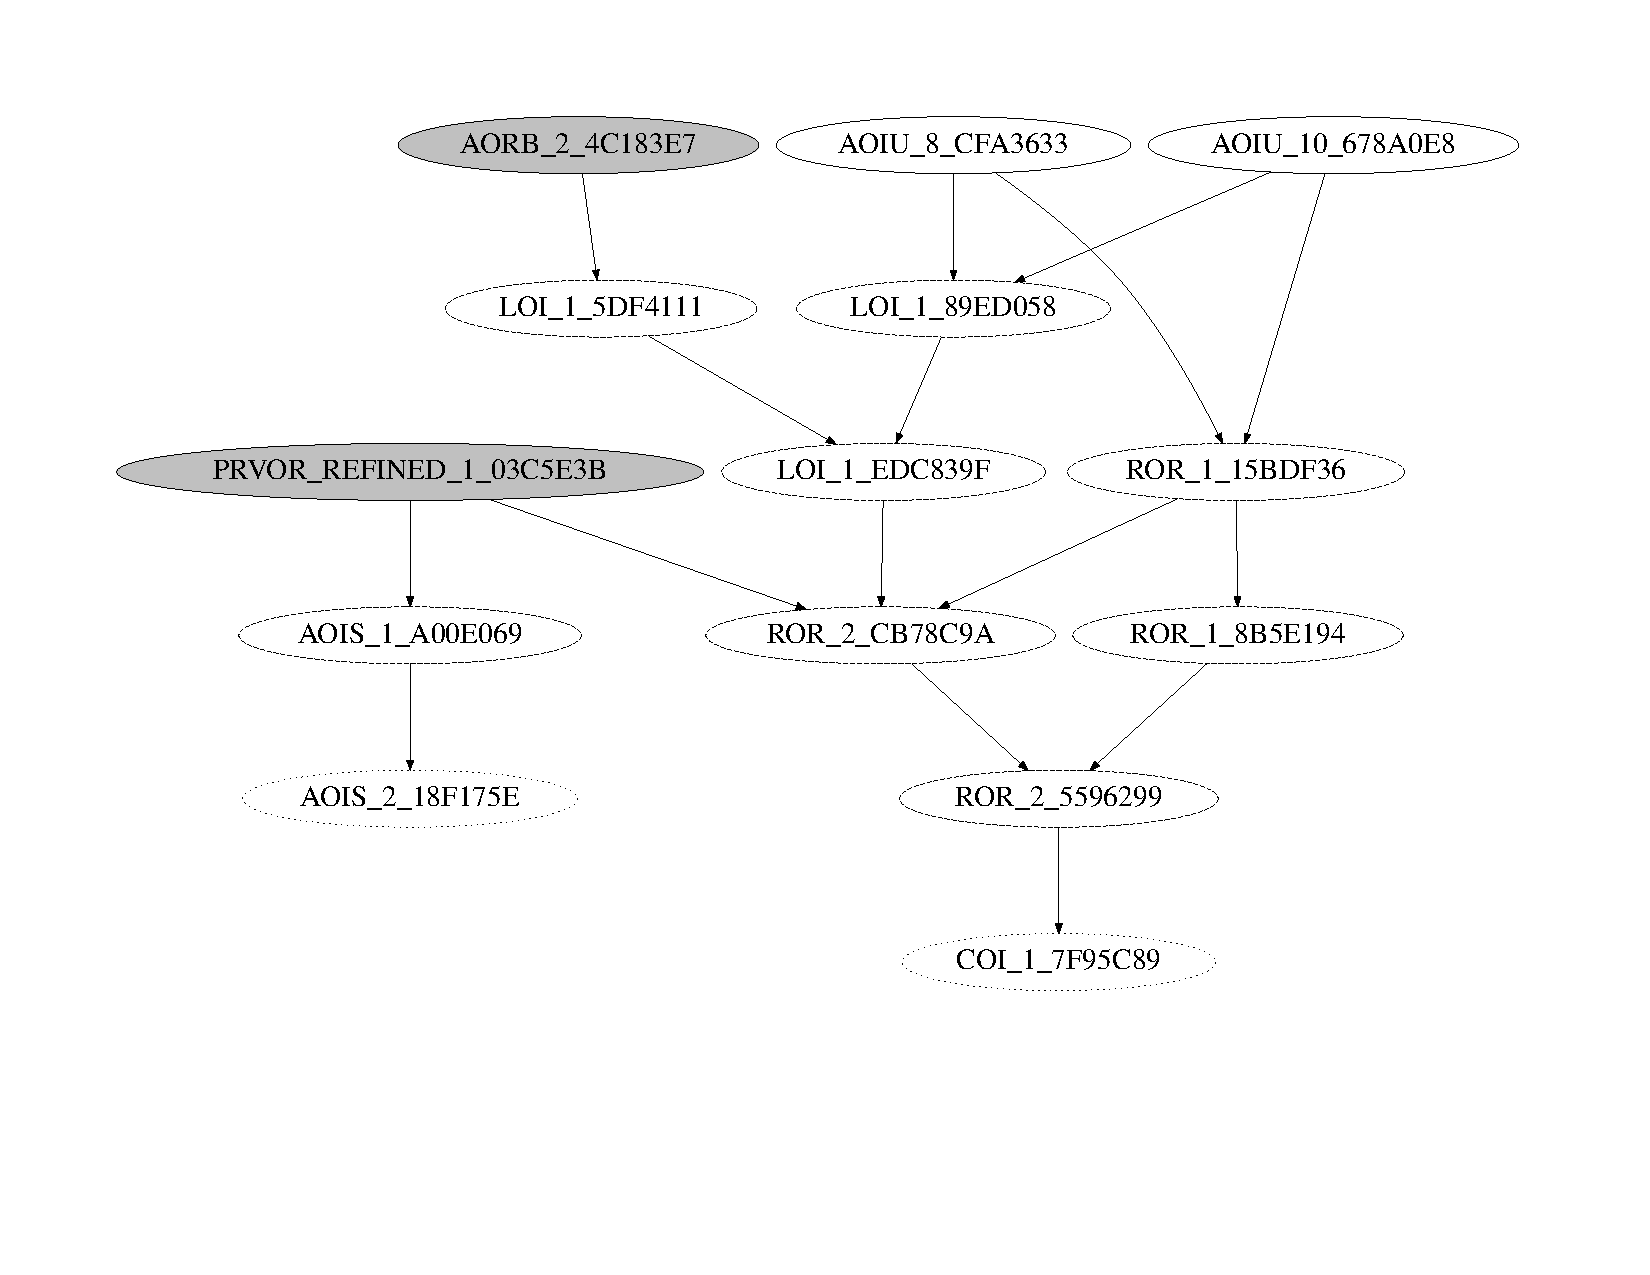
\includegraphics[width=\linewidth]{figures/subsumption/dsg_apache_prvo_segment.pdf}
	\caption[Grafo de subsunci\'on para mutantes \emph{PRVO} de \emph{TreeList}]{Grafo reducido de \emph{Dynamic Mutant Subsumption} para \emph{TreeList} con \emph{PRVO}.}
	\label{figures.examples.subsumption.reducedTreeListGraph}
\end{figure}

Las conclusiones sobre los resultados obtenidos no solamente se basan en la cantidad de nodos dominantes puros que genera \emph{PRVO}, sino tambi\'en en la relaci\'on entre los nodos dominantes donde participan los operadores suficientes con y sin la inclusi\'on de \emph{PRVO}. Principalmente, si la cantidad promedio de nodos dominantes de otros operadores aumentara al agregar \emph{PRVO}, la intuici\'on ser\'ia que \emph{PRVO} est\'a siendo subsumido. Esta situaci\'on no solo que no se observa en la mayor\'ia de los casos, sino que se observa la situaci\'on opuesta, es decir, la cantidad de nodos dominantes donde participan los operadores suficientes disminuye. Esto tomado en conjunto con el hecho de que \emph{PRVO} participa en una gran cantidad de nodos dominantes, y que a su vez suele hacerlo de manera independiente, es decir, la mayor\'ia de los nodos dominantes donde participa son puros, lleva a considerar que \emph{PRVO} estar\'ia dominando a los mutantes generados por los operadores suficientes.

En general, la observaci\'on m\'as importante al analizar los resultados es que, en casi todos los casos (con la excepci\'on de \emph{NodeCachingList}), \emph{PRVO} se posiciona entre los mejores, con respecto a dominancia, incluso es uno de los mejores tres operadores dominantes, junto a operadores t\'ipicos del conjunto de \emph{suficientes}, como \emph{ROR}, \emph{LOI}, y la familia de operadores de mutaci\'on que corresponden a la inserci\'on de operadores aritm\'eticos (\emph{AOIS}, \emph{AOIU}, y \emph{AOIB}). Es tambi\'en importante de remarcar que, en presencia de \emph{PRVO}, la dominancia de otros operadores es en general reducida, y su dominancia sobre ciertos nodos es ``transferida'' hacia \emph{PRVO}. M\'as precisamente, \emph{PRVO} domina sobre ciertos mutantes previamente (en ausencia de \emph{PRVO}) dominantes.

Un an\'alisis m\'as profundo de los resultados obtenidos con respecto a mutantes dominantes, nos lleva a dividir a \'estos en tres conjuntos. Para \emph{AvlTree}, \emph{Queue}, y \emph{BSTree}, al agregar \emph{PRVO} se obtiene una gran cantidad de nodos dominantes puros al tiempo que los nodos dominantes donde participan los operadores suficientes disminuye de manera considerable. En estos casos la participaci\'on en nodos dominantes por parte de los otros operadores llega a disminuir en algunos casos a la mitad. Para \emph{TreeList} y \emph{BinomialHeap} la dominancia de \emph{PRVO} sobre los operadores suficientes es menos notable, incluso viendo algunos casos donde la participaci\'on en nodos dominantes por parte de operadores, como \emph{AOIS}, incrementa. Finalmente el peor caso para \emph{PRVO} es \emph{NodeCachingList} donde salvo para los operadores \emph{COI} y \emph{AORS}, la participaci\'on en nodos dominantes por parte de los operadores suficientes incrementa. Sin embargo, en todos los casos \emph{PRVO} da a lugar a nodos dominantes puros, lo que indica que nunca llega a ser redundante.

Claramente, nuestros resultados experimentales resultan en una respuesta positiva a \textbf{RQ1}: \emph{PRVO} complementa de manera significativa al conjunto de operadores tradicionales; los mutantes producidos son en general no dominados por operadores existentes, y exhibe un alto n\'umero de mutantes dominantes, lo que nos permitir\'ia considerar, al menos en el contexto de nuestros experimentos, a \emph{PRVO} como un operador ``suficiente'', junto al conjunto de operadores suficientes tradicionales.

\begin{figure}[t]
	\begin{center}
		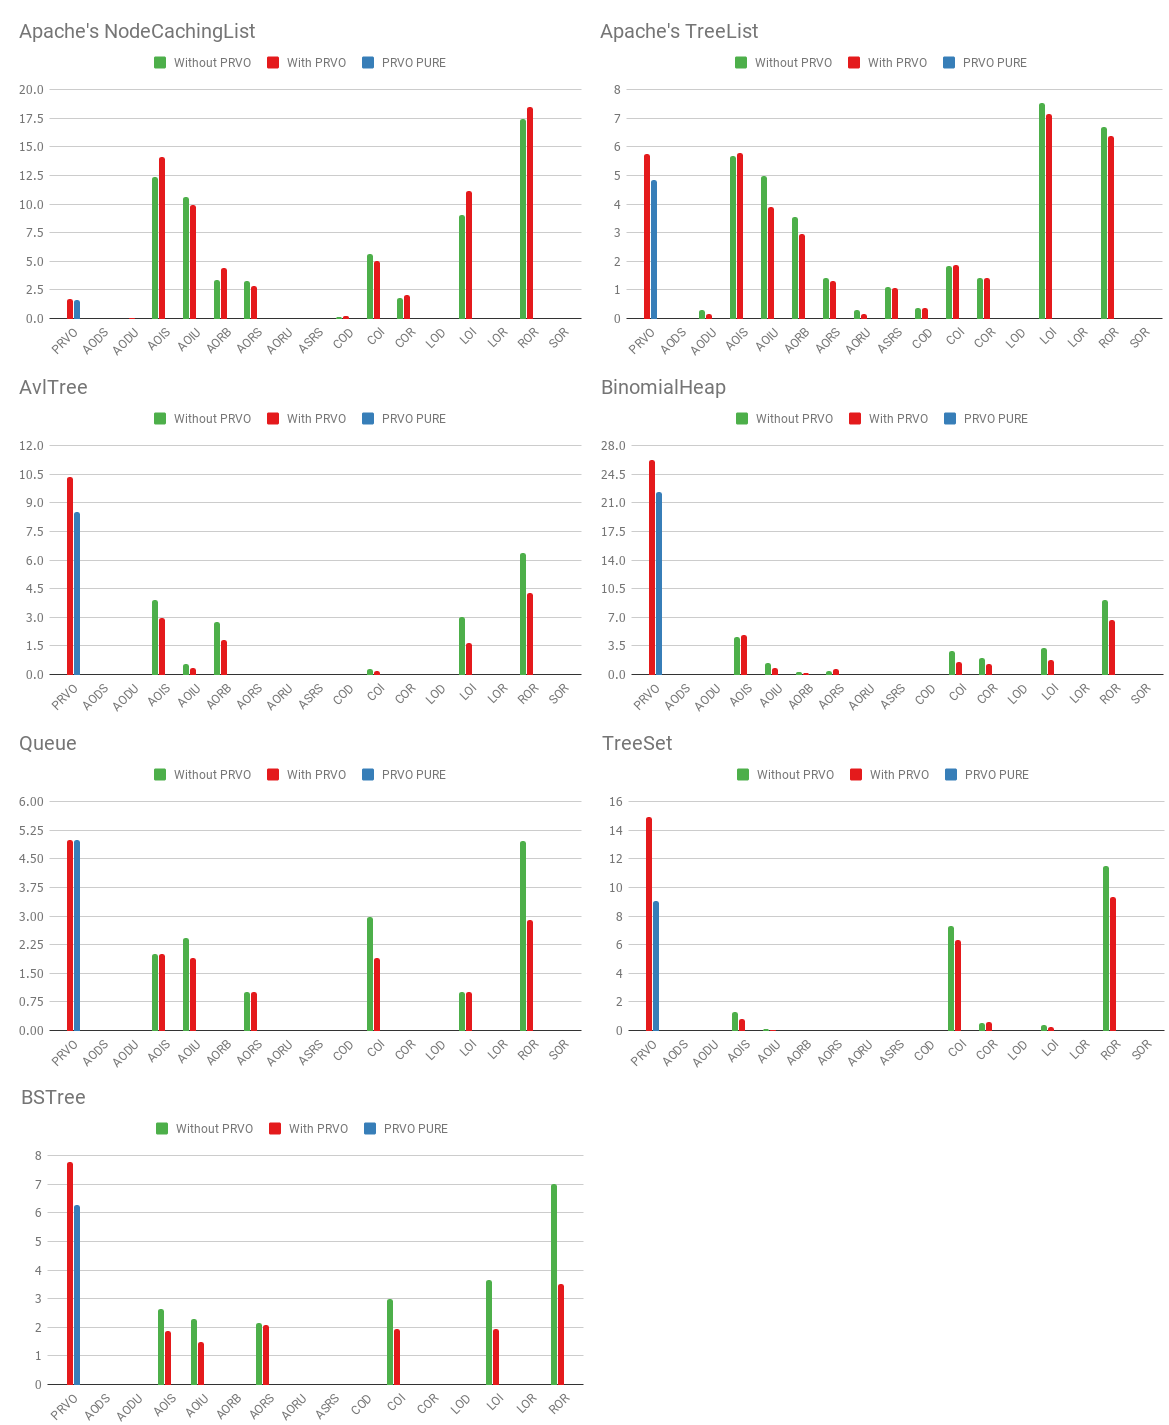
\includegraphics[width=12cm]{figures/Tables.png}
	\end{center}
	\caption{Resultados del an\'alsis de \emph{dynamic subsumption analysis}}
	\label{subsumption-results}
\end{figure}

Analicemos ahora \textbf{RQ2}. La Figura~\ref{mutants-results} y la Tabla \ref{tables.results.equivalents} resumen los resultados para generaci\'on de mutantes, comparando el n\'umero de mutantes obtenidos cuando \emph{PRVO} no es inclu\'ido (barras verdes), con los casos en donde \emph{PRVO} es considerado (barras azules). Reportamos tambi\'en, el n\'umero de mutantes equivalentes de \emph{PRVO} (mutantes que son sem\'anticamente equivalentes al programa original, y por lo tanto imposibles de detectar con cualquier test) producidos para cada caso de estudio.

Para la mayor\'ia de los casos de estudio, el n\'umero de mutantes que genera \emph{PRVO} representa solo un peque\~no incremento sobre la cantidad de mutantes generados por los operadores tradicionales. Los casos de estudio \emph{TreeSet} y \emph{BinomialHeap} son dos excepciones, en donde la cantidad de mutantes generados por \emph{PRVO} representa pr\'acticamente la misma que la generada por todos los operadores tradicionales por si solos. La raz\'on es que estos casos de estudios se caracterizan por una gran cantidad de m\'etodos, que a su vez contienen una gran cantidad de expresiones de navegaci\'on en condiciones y otras comparaciones, del tipo \texttt{expr == null}. Estas expresiones admiten una sola mutaci\'on de parte de \emph{ROR} (reemplazar el igual por un distinto), pero en donde \emph{PRVO} produce muchas mutaciones. Sin embargo, en estos dos estudios, hay que notar que \emph{PRVO} es claramente dominante (como se ve en la Figura~\ref{subsumption-results}); en particular, es notable como la dominancia de otros operadores es disminu\'ida significativamente cuando \emph{PRVO} es utilizado. Nuestra respuesta entonces para \textbf{RQ2}, es que el costo adicional, con respecto a cantidad de mutantes, de utilizar \emph{PRVO}, es en general bajo, aunque existen casos en donde el n\'umero de mutaciones generadas por \emph{PRVO} puede ``explotar''. Estos casos muestran, en nuestros experimentos, una gran dominancia por parte de \emph{PRVO} sobre mutaciones producidas por otros operadores, sugiriendo que existe un margen para realizar optimizaciones mediante priorizaci\'on de tests/mutantes, una t\'ecnica que consiste en ordenar y/o seleccionar tests o mutantes para ser evaluados antes, o en lugar, de otros, para as\'i disminuir los recursos necesarios. De todas formas, estos resultados sugieren realizar refinamientos a \emph{PRVO}, ya sea a\~nadiendo an\'alisis durante la generaci\'on de mutaciones, o implementando nuevas propiedades para configurar a \emph{PRVO} de manera m\'as apropiada para cada caso. Esto, puede llevar a lograr una mejor eficiencia, es decir una menor cantidad de mutantes, por parte de \emph{PRVO}.

Con respecto a mutantes equivalentes, los resultados son muy interesantes. La cantidad de mutantes equivalentes producidos por \emph{PRVO} fue muy poca. Esto, es muy importante, dado que cuando un operador produce muchos mutantes equivalentes: mutantes para los cuales no existe ning\'un escenario o entrada para el cual \'este se comporte de manera diferente al programa original, lo que lo hace imposible de detectar; el valor de mutation score correspondiente disminuye de manera artificial, resultando en una evaluaci\'on enga\~nosa del test suite. Tener entonces una peque\~na cantidad de dichos mutantes es un buen resultado para \emph{PRVO}. Vale la pena aclarar que si bien lo deseable es evitar por completo la generaci\'on de mutantes equivalentes, esto es en general imposible, principalmente por que al ser un problema indecidible (el detectar si un programa es equivalente a otro), no es posible tener una implementaci\'on de una herramienta de mutaci\'on que evite por completo la generaci\'on de los mismos.

El an\'alisis de \emph{Dynamic Mutant Subsumption} representa un estudio m\'as profundo que permite analizar informaci\'on que suele estar oculta cuando solo se calcula mutation score. El hecho de que \emph{PRVO} domine con respecto a este an\'alisis significa que se generan mutantes que son detectados, por lo tanto el mutation score no deber\'ia disminuir. De la misma forma, la dominancia por parte de \emph{PRVO} no es compatible con una disminuci\'on de la ``dureza'' promedio para detectar a los mutantes. Esto es confirmado por los resultados obtenidos de \emph{Mutation Score} \ref{mutationscore-results}, \emph{Toughness} \ref{toughness-results}, y \emph{Toughness de solo detectados} \ref{toughnessKilled-results}, que se condicen con los resultados de dominancia y mutantes equivalentes generados por \emph{PRVO}. El mutation score al utilizar \emph{PRVO} (en color rojo) se mantiene en general levemente por encima del obtenido al utilizar solamente los operadores suficientes (en color verde), esto junto a los resultados de dominancia, indica que la cantidad de mutantes triviales generados por \emph{PRVO} es poca (lo que llevar\'ia a un aumento del mutation score), y que la generaci\'on de mutantes equivalentes tambi\'en lo es, dado que \'estos llevar\'ian a una disminuci\'on del valor de mutation score obtenido.

Los resultados de \emph{Toughness}, tanto si se consideran todos los mutantes o solo se consideran aquellos que fueron detectados, apoyan la conclusi\'on anterior de que \emph{PRVO} no solo que no genera mutantes triviales, sino que adem\'as, \'estos son en general dif\'iciles de matar. La utilizaci\'on de test suites conformadas por una gran cantidad de tests con mayormente una cobertura de ramas alta \ref{testsAndCov-results} (lo que podr\'ia llevar a considerar a \'estas como ``suficientemente buenas'') permitir\'ia considerar como stubborn a los mutantes de \emph{PRVO} que sobrevivieron y no fueron determinados como equivalentes.

\begin{table}[]
	\caption[Casos de estudio, tests y cobertura de ramas]{Cantidad promedio de tests y cobertura de ramas para cada caso de estudio.}
	\label{testsAndCov-results}
	\centering
	\footnotesize
	\def\arraystretch{1.1}
	\setlength\tabcolsep{0.9mm}
	\begin{tabular}{|c|c|c|c|c|c|c|c|c|}
		\hline
		Project & TreeList & AvlTree & BinHeap & Queue & TreeSet & NCLL & BSTree & OrdSet\\ \cline{1-1}
		Tests & 2310 & 3391 & 3274 & 3307 & 3452 & 3819 & 3178 & 3601\\ \cline{1-1}
		Branch Cov & 100\% & 100\% & 90.3\% & 87\% & 89.46\% & 96.56\% & 94\% & 91.1\%\\ \hline
	\end{tabular}
\end{table}

\begin{figure}
	\begin{center}
		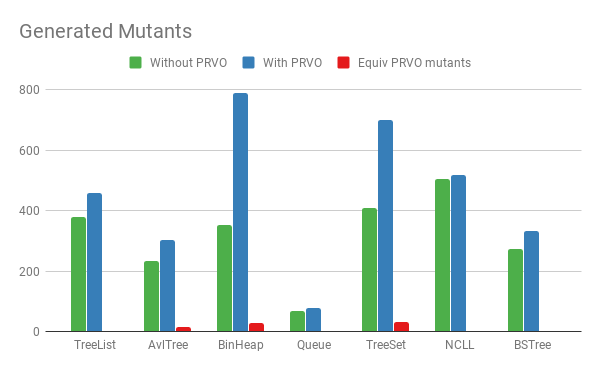
\includegraphics[width=9cm]{figures/Generated_Mutants.png}
	\end{center}
	\caption{Comparaci\'on de mutantes generados.}
	\label{mutants-results}
\end{figure}


\begin{figure}
	\begin{center}
		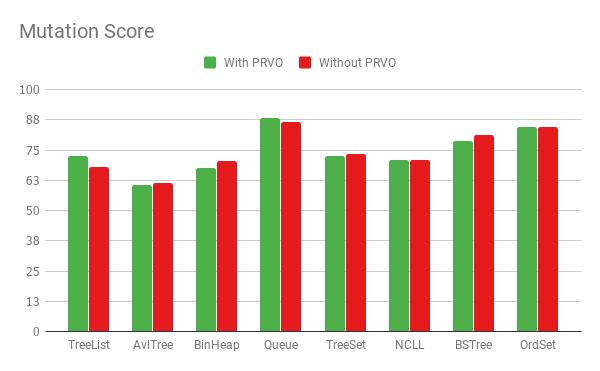
\includegraphics[width=9cm]{figures/MutationScore.png}
	\end{center}
	\caption{Comparaci\'on de \emph{Mutation score}.}
	\label{mutationscore-results}
\end{figure}

\begin{figure}
	\begin{center}
		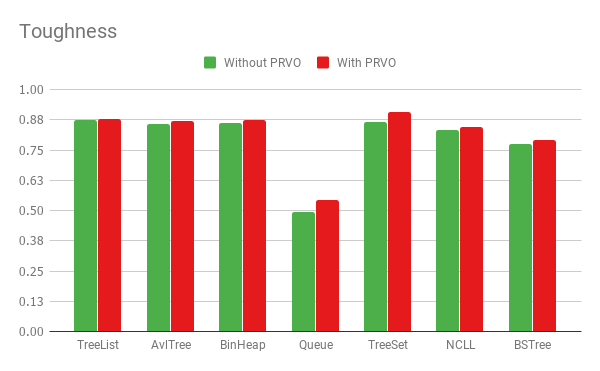
\includegraphics[width=9cm]{figures/Toughness.png}
	\end{center}
	\caption[Comparaci\'on de \emph{Toughness}]{Comparaci\'on de \emph{Toughness}, cuantos tests ``resiste'' un mutante para ser detectado, un valor de $1.0$ representa un mutante no detectado.}
	\label{toughness-results}
\end{figure}

\begin{figure}
	\begin{center}
		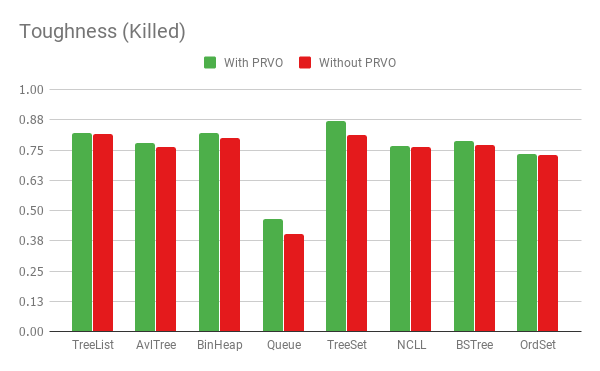
\includegraphics[width=9cm]{figures/ToughnessKilled.png}
	\end{center}
	\caption[Comparaci\'on de \emph{Toughness Killed}]{Comparaci\'on de \emph{Toughness Killed}, cuantos tests ``resiste'' un mutante que fue detectado.}
	\label{toughnessKilled-results}
\end{figure}


\section{Amenazas a la validez}

Nuestra evaluaci\'on experimental est\'a limitada a implementaciones relativamente peque\~nas de colecciones en \emph{Java}. Las razones por las que seleccionamos estas implementaciones como casos de estudio fueron parcialmente descriptas anteriormente, y esencialmente tiene que ver con que estos proyectos son buenos representantes de implementaciones orientadas a objetos con usos sofisticados de expresiones de navegaci\'on (por ejemplo, utilizan tipos de datos recursivos, y m\'ultiples referencias a objetos distintos del mismo tipo). Otra raz\'on por la que nos limitamos a estos casos de estudio tiene que ver con el alto costo de an\'alisis de mutaci\'on. Especialmente en nuestro contexto, en donde las caracter\'isticas de nuestra evaluaci\'on nos lleva a la necesidad de realizar numerosos an\'alisis de mutaci\'on, en particular, computar los grafos de subsunci\'on de mutantes har\'ia inviable esta evaluaci\'on si fu\'eramos a utilizar proyectos m\'as grandes.

Nuestro an\'alisis est\'a tambi\'en atado a una forma espec\'ifica de generar tests, \'esta se basa en el uso de dos herramientas particulares, Evosuite y Randoop espec\'ificamente. Esto est\'a motivado por el tipo de test suites que resultan de relevancia para an\'alisis de dynamic mutant subsumption. Dado el impacto que tiene el presupuesto de tiempo que se brinda a las herramientas que utilizamos para generar las test suites, nuestros resultados podr\'ian estar siendo afectados por el mismo. Para contrarrestar esta potencial amenaza, corrimos los experimentos con distintos presupuestos de tiempo, lo que llev\'o a test suites de distintos tama\~nos, pero sin embargo no obtuvimos resultados diferentes. El costo de tiempo llev\'o a realizar esta evaluaci\'on previa en un subconjunto de los casos de estudio.

La mayor parte de nuestra evaluaci\'on experimental es objetiva, es decir, provienen de an\'alisis algor\'itmicos  que retornan un valor particular, por ejemplo la noci\'on de dynamic mutant subsumption y la cantidad de mutantes generados, \'estas est\'an calculadas por nuestra implementaci\'on de \emph{$\mu$Java++} o por los scripts utilizados para automatizar los experimentos. Hicimos nuestro mejor esfuerzo para garantizar la validez de nuestros resultados, pero a\'un as\'i nuestra implementaci\'on podr\'ia contener defectos que afecten a nuestros resultados. En contraposici\'on, la equivalencia de programas, requerida para analizar mutantes equivalentes, es un problema indecidible. Varias t\'ecnicas han sido propuestas para resolver este problema (obviamente de manera aproximada), sin embargo, la verificaci\'on manual sigue siendo una de las m\'as utilizada en la pr\'actica, y es la que hemos utilizados nosotros. Afortunadamente este an\'alisis estuvo limitado a un n\'umero muy peque\~no de mutantes y cualquier duda sobre la equivalencia de uno, fue siempre anotada en desventaja de \emph{PRVO}, es decir, ante la duda, se consider\'o el mutante como equivalente. Creemos que los errores que podemos haber cometido con respecto a equivalencia de mutantes, no afectan de manera significativa nuestras conclusiones.

Nuestro an\'alisis est\'a tambi\'en limitado a un conjunto arbitrario de operadores de mutaci\'on. Podr\'iamos haber considerado otros operadores, por ejemplo los que act\'uan a nivel de clases (en contraposici\'on de los que usamos que act\'uan a nivel de m\'etodos) \cite{bibliography.mutation.class-level-ops}. \'Estos, est\'an relacionados a nuestro trabajo, en el sentido de que se aplican a programas orientados a objetos, pero se enfocan en aspectos ortogonales como visibilidad (cambiando la visibilidad de m\'etodos y campos en una clase). Decidimos concentrarnos en los operadores que se consideran tradicionales, en el contexto de mutation testing, y creemos que hemos tenido en cuenta a los m\'as significativos, basado en los que est\'an disponibles en las herramientas de mutation testing, y en estudios de operadores suficientes.

%Finalmente necesitamos remarcar que la relaci\'on de subsunci\'on de operadores, no es lo mismo que la subsunci\'on de mutantes. El primero es una relaci\'on entre operadores que es independiente de que programa se est\'e mutando, se trata de una relaci\'on que o bien se explica por la misma definici\'on de los operadores, o bien (como sucede en la mayor\'ia de los casos) requiere numerosos experimentos para determinar si es posible concluir si un operador subsume a otro. Sin embargo nuestra evaluaci\'on de subsuma din\'amica de mutantes, permite, de manera indirecta, una evaluaci\'on de la primera.

\begin{table}[]
	\caption{Mutantes generados por caso de estudio}
	\label{tables.results.mutants}
	\centering
	\footnotesize
	\def\arraystretch{1.1}
	\setlength\tabcolsep{1.0mm}
	\begin{tabular}{l|cccccccc|}
		\cline{2-9}
		& \multicolumn{1}{l}{TreeList} & \multicolumn{1}{l}{AvlTree} & \multicolumn{1}{l}{BinHeap} & \multicolumn{1}{l}{Queue} & \multicolumn{1}{l}{TreeSet} & \multicolumn{1}{l}{NCLL} & \multicolumn{1}{l}{BSTree} & \multicolumn{1}{l|}{OrdSet} \\ \hline
		\multicolumn{1}{|l|}{Sin PRVO} & 380 & 233 & 352 & 68 & 410 & 504 & 274 & 1208\\ \cline{1-1}
		\multicolumn{1}{|l|}{Con PRVO} & 458 & 304 & 788 & 78 & 700 & 519 & 334 & 1296\\ \hline
	\end{tabular}
\end{table}

\begin{table}[]
	\caption{Mutantes \emph{PRVO} equivalentes por caso de estudio}
	\label{tables.results.equivalents}
	\centering
	\footnotesize
	\def\arraystretch{1.1}
	\setlength\tabcolsep{0.5mm}
	\begin{tabular}{l|cccccccc|}
		\cline{2-9}
		& \multicolumn{1}{l}{TreeList} & \multicolumn{1}{l}{AvlTree} & \multicolumn{1}{l}{BinHeap} & \multicolumn{1}{l}{Queue} & \multicolumn{1}{l}{TreeSet} & \multicolumn{1}{l}{NCLL} &
		\multicolumn{1}{l}{BSTree} & \multicolumn{1}{l|}{OrdSet}\\ \hline
		\multicolumn{1}{|l|}{Mutantes totales} & 78 & 71 & 436 & 10 & 290 & 15 & 60 & 88\\ \cline{1-1}
		\multicolumn{1}{|l|}{Equivalentes} & 2 & 14 & 27 & 0 & 31 & 2 & 2 & 9\\ \hline
	\end{tabular}
\end{table}

\begin{table}[]
	\caption[\emph{Dynamic Mutant Subsumption} \emph{TreeList}, sin \emph{PRVO}]{Resultados de \emph{Dynamic Mutant Subsumption} para \emph{TreeList}, sin \emph{PRVO}}
	\label{tables.results.subsumption.treelist.noprvo}
	\centering
	\scriptsize
	\def\arraystretch{0.95}
	\setlength\tabcolsep{0.5mm}
	\begin{tabular}{rrrrrrrrrrrrr}
		DOM NODES & AODU & AOIS & AOIU & AORB & AORS & AORU & ASRS & COD & COI & COR & LOI & ROR \\
		24 & 0 & 10 & 3 & 4 & 2 & 0 & 1 & 0 & 1 & 1 & 8 & 6 \\
		23 & 0 & 8 & 4 & 2 & 1 & 0 & 0 & 0 & 2 & 1 & 7 & 5 \\
		21 & 0 & 4 & 4 & 3 & 1 & 0 & 1 & 1 & 3 & 2 & 9 & 7 \\
		16 & 0 & 5 & 2 & 3 & 1 & 0 & 1 & 1 & 1 & 0 & 8 & 5 \\
		21 & 0 & 5 & 7 & 5 & 1 & 0 & 1 & 1 & 3 & 2 & 7 & 7 \\
		23 & 0 & 8 & 6 & 4 & 2 & 0 & 1 & 1 & 3 & 3 & 11 & 6 \\
		23 & 0 & 4 & 7 & 2 & 1 & 0 & 2 & 1 & 3 & 2 & 9 & 7 \\
		23 & 0 & 6 & 4 & 3 & 2 & 0 & 1 & 1 & 3 & 3 & 10 & 7 \\
		26 & 0 & 8 & 2 & 3 & 0 & 0 & 1 & 0 & 1 & 0 & 8 & 7 \\
		22 & 0 & 6 & 6 & 3 & 2 & 0 & 1 & 0 & 3 & 1 & 8 & 7 \\
		15 & 1 & 5 & 6 & 3 & 2 & 1 & 0 & 0 & 4 & 2 & 7 & 8 \\
		27 & 0 & 7 & 4 & 4 & 2 & 0 & 2 & 1 & 3 & 3 & 8 & 9 \\
		19 & 0 & 4 & 5 & 4 & 1 & 0 & 1 & 1 & 3 & 3 & 9 & 7 \\
		19 & 1 & 5 & 6 & 5 & 1 & 1 & 1 & 0 & 4 & 2 & 8 & 8 \\
		24 & 0 & 8 & 5 & 4 & 1 & 0 & 0 & 0 & 2 & 1 & 8 & 7 \\
		21 & 0 & 5 & 8 & 4 & 1 & 0 & 2 & 1 & 1 & 3 & 8 & 7 \\
		23 & 1 & 7 & 5 & 2 & 1 & 1 & 1 & 0 & 2 & 0 & 6 & 7 \\
		25 & 1 & 6 & 4 & 4 & 0 & 1 & 1 & 0 & 3 & 2 & 9 & 10 \\
		22 & 0 & 6 & 4 & 2 & 1 & 0 & 3 & 1 & 2 & 1 & 8 & 6 \\
		19 & 0 & 6 & 4 & 3 & 1 & 0 & 2 & 1 & 1 & 2 & 8 & 4 \\
		26 & 0 & 4 & 5 & 2 & 2 & 0 & 1 & 0 & 2 & 2 & 7 & 9 \\
		23 & 0 & 6 & 6 & 3 & 0 & 0 & 2 & 0 & 1 & 1 & 6 & 9 \\
		17 & 0 & 1 & 5 & 4 & 0 & 0 & 0 & 0 & 1 & 2 & 4 & 7 \\
		26 & 1 & 6 & 4 & 2 & 0 & 1 & 0 & 0 & 3 & 2 & 6 & 11 \\
		23 & 0 & 7 & 6 & 4 & 1 & 0 & 2 & 0 & 2 & 1 & 7 & 6 \\
		20 & 0 & 7 & 3 & 2 & 0 & 0 & 2 & 0 & 0 & 0 & 9 & 7 \\
		21 & 1 & 2 & 7 & 4 & 1 & 1 & 1 & 1 & 3 & 2 & 7 & 9 \\
		22 & 0 & 4 & 5 & 5 & 2 & 0 & 3 & 0 & 0 & 0 & 7 & 6 \\
		24 & 0 & 8 & 3 & 3 & 1 & 0 & 1 & 0 & 2 & 1 & 8 & 7 \\
		22 & 0 & 6 & 5 & 4 & 2 & 0 & 1 & 0 & 2 & 0 & 8 & 4
	\end{tabular}
\end{table}

\begin{table}[]
	\caption[\emph{Dynamic Mutant Subsumption} \emph{TreeList}, con \emph{PRVO}]{Resultados de \emph{Dynamic Mutant Subsumption} para \emph{TreeList}, con \emph{PRVO}}
	\label{tables.results.subsumption.treelist.prvo}
	\centering
	\scriptsize
	\def\arraystretch{0.95}
	\setlength\tabcolsep{0.5mm}
	\begin{tabular}{rrrrrrrrrrrrrr}
		DOM NODES & PRVO & AODU & AOIS & AOIU & AORB & AORS & AORU & ASRS & COD & COI & COR & LOI & ROR \\
		15 & 4 & 1 & 5 & 6 & 3 & 2 & 1 & 0 & 0 & 4 & 2 & 7 & 8 \\
		22 & 4 & 0 & 4 & 5 & 4 & 1 & 0 & 1 & 1 & 3 & 3 & 9 & 7 \\
		30 & 8 & 0 & 8 & 3 & 4 & 1 & 0 & 0 & 0 & 2 & 1 & 7 & 7 \\
		22 & 4 & 0 & 3 & 7 & 4 & 1 & 0 & 2 & 1 & 1 & 3 & 7 & 7 \\
		21 & 6 & 0 & 4 & 3 & 3 & 1 & 0 & 1 & 1 & 2 & 2 & 7 & 6 \\
		24 & 7 & 0 & 4 & 7 & 2 & 1 & 0 & 2 & 1 & 3 & 2 & 8 & 6 \\
		27 & 6 & 0 & 6 & 6 & 3 & 2 & 0 & 1 & 0 & 3 & 1 & 8 & 7 \\
		33 & 8 & 0 & 8 & 2 & 3 & 0 & 0 & 1 & 0 & 1 & 0 & 8 & 7 \\
		28 & 8 & 1 & 3 & 3 & 3 & 0 & 1 & 1 & 0 & 2 & 1 & 7 & 9 \\
		24 & 6 & 1 & 2 & 7 & 4 & 1 & 1 & 1 & 1 & 2 & 2 & 7 & 7 \\
		20 & 2 & 1 & 5 & 6 & 5 & 1 & 1 & 1 & 0 & 4 & 2 & 8 & 8 \\
		29 & 7 & 0 & 6 & 5 & 3 & 0 & 0 & 2 & 0 & 1 & 1 & 6 & 9 \\
		28 & 4 & 0 & 8 & 3 & 3 & 1 & 0 & 1 & 0 & 2 & 1 & 8 & 7 \\
		26 & 5 & 0 & 7 & 4 & 4 & 1 & 0 & 2 & 0 & 2 & 1 & 7 & 6 \\
		27 & 5 & 0 & 8 & 4 & 2 & 1 & 0 & 0 & 0 & 2 & 1 & 7 & 5 \\
		35 & 10 & 1 & 6 & 3 & 2 & 0 & 1 & 0 & 0 & 3 & 2 & 6 & 11 \\
		24 & 9 & 0 & 5 & 1 & 3 & 1 & 0 & 1 & 1 & 1 & 0 & 8 & 5 \\
		23 & 8 & 0 & 1 & 3 & 3 & 0 & 0 & 0 & 0 & 1 & 2 & 4 & 7 \\
		32 & 7 & 0 & 7 & 3 & 3 & 2 & 0 & 2 & 1 & 3 & 3 & 8 & 9 \\
		22 & 4 & 0 & 5 & 3 & 2 & 0 & 0 & 2 & 0 & 0 & 0 & 9 & 7 \\
		22 & 5 & 0 & 5 & 3 & 3 & 2 & 0 & 1 & 1 & 3 & 3 & 7 & 6 \\
		24 & 5 & 0 & 8 & 5 & 4 & 2 & 0 & 1 & 1 & 1 & 3 & 9 & 5 \\
		25 & 5 & 0 & 4 & 4 & 4 & 2 & 0 & 3 & 0 & 0 & 0 & 7 & 6 \\
		24 & 6 & 0 & 9 & 2 & 3 & 1 & 0 & 1 & 0 & 1 & 1 & 7 & 4 \\
		27 & 5 & 0 & 6 & 4 & 2 & 1 & 0 & 3 & 1 & 2 & 1 & 8 & 6 \\
		23 & 5 & 0 & 6 & 4 & 3 & 1 & 0 & 2 & 1 & 1 & 2 & 8 & 4 \\
		31 & 6 & 0 & 4 & 5 & 2 & 2 & 0 & 1 & 0 & 2 & 2 & 7 & 9 \\
		25 & 7 & 0 & 6 & 4 & 4 & 2 & 0 & 1 & 0 & 2 & 0 & 7 & 4 \\
		25 & 5 & 0 & 5 & 6 & 5 & 1 & 0 & 1 & 1 & 3 & 2 & 6 & 7 \\
		29 & 7 & 1 & 7 & 4 & 2 & 1 & 1 & 1 & 0 & 2 & 0 & 6 & 7
	\end{tabular}
\end{table}

\begin{table}[]
	\caption[\emph{Dynamic Mutant Subsumption} \emph{AvlTree}, sin \emph{PRVO}]{Resultados de \emph{Dynamic Mutant Subsumption} para \emph{AvlTree}, sin \emph{PRVO}}
	\label{tables.results.subsumption.avltree.noprvo}
	\centering
	\scriptsize
	\def\arraystretch{0.95}
	\setlength\tabcolsep{0.5mm}
	\begin{tabular}{rrrrrrr}
		DOM NODES & AOIS & AOIU & AORB & COI & LOI & ROR \\
		13 & 2 & 0 & 3 & 1 & 3 & 6 \\
		17 & 6 & 0 & 2 & 1 & 5 & 6 \\
		21 & 5 & 1 & 4 & 1 & 4 & 8 \\
		21 & 7 & 1 & 4 & 1 & 4 & 7 \\
		21 & 5 & 1 & 3 & 0 & 4 & 9 \\
		19 & 5 & 0 & 4 & 1 & 4 & 8 \\
		20 & 7 & 0 & 4 & 0 & 3 & 8 \\
		16 & 5 & 0 & 3 & 0 & 3 & 5 \\
		23 & 9 & 3 & 3 & 0 & 2 & 6 \\
		12 & 2 & 0 & 4 & 0 & 3 & 4 \\
		17 & 4 & 0 & 2 & 0 & 2 & 11 \\
		14 & 2 & 0 & 4 & 0 & 3 & 5 \\
		17 & 4 & 1 & 3 & 0 & 3 & 7 \\
		21 & 4 & 2 & 3 & 0 & 3 & 10 \\
		12 & 7 & 0 & 2 & 0 & 1 & 3 \\
		13 & 2 & 0 & 3 & 1 & 3 & 6 \\
		23 & 6 & 2 & 4 & 0 & 5 & 7 \\
		13 & 4 & 0 & 4 & 0 & 2 & 4 \\
		21 & 7 & 1 & 3 & 0 & 5 & 7 \\
		19 & 4 & 1 & 4 & 0 & 4 & 7 \\
		21 & 7 & 1 & 4 & 1 & 2 & 8 \\
		21 & 6 & 0 & 4 & 0 & 4 & 9 \\
		19 & 7 & 1 & 3 & 1 & 3 & 7 \\
		22 & 7 & 1 & 2 & 0 & 6 & 8 \\
		13 & 2 & 1 & 3 & 1 & 4 & 5 \\
		15 & 5 & 0 & 2 & 0 & 4 & 6 \\
		17 & 3 & 1 & 3 & 0 & 5 & 7 \\
		11 & 2 & 0 & 3 & 0 & 3 & 4 \\
		17 & 4 & 1 & 3 & 1 & 4 & 6 \\
		22 & 8 & 1 & 3 & 0 & 4 & 7
	\end{tabular}
\end{table}

\begin{table}[]
	\caption[\emph{Dynamic Mutant Subsumption} \emph{AvlTree}, con \emph{PRVO}]{Resultados de \emph{Dynamic Mutant Subsumption} para \emph{AvlTree}, con \emph{PRVO}}
	\label{tables.results.subsumption.avltree.prvo}
	\centering
	\scriptsize
	\def\arraystretch{0.95}
	\setlength\tabcolsep{0.5mm}
	\begin{tabular}{rrrrrrrr}
		DOM NODES & PRVO & AOIS & AOIU & AORB & COI & LOI & ROR \\
		23 & 9 & 5 & 1 & 2 & 0 & 2 & 5 \\
		18 & 8 & 2 & 0 & 3 & 0 & 1 & 5 \\
		19 & 8 & 3 & 1 & 1 & 0 & 4 & 4 \\
		21 & 10 & 3 & 1 & 2 & 0 & 2 & 5 \\
		19 & 11 & 2 & 0 & 4 & 0 & 1 & 3 \\
		19 & 9 & 2 & 0 & 3 & 0 & 1 & 4 \\
		20 & 12 & 3 & 0 & 2 & 0 & 1 & 4 \\
		21 & 4 & 5 & 2 & 3 & 0 & 2 & 6 \\
		25 & 15 & 5 & 0 & 1 & 0 & 2 & 4 \\
		21 & 11 & 4 & 0 & 2 & 1 & 2 & 5 \\
		21 & 13 & 4 & 0 & 0 & 0 & 0 & 6 \\
		25 & 10 & 4 & 2 & 3 & 0 & 1 & 7 \\
		21 & 10 & 6 & 1 & 2 & 0 & 1 & 3 \\
		16 & 7 & 4 & 0 & 2 & 0 & 1 & 4 \\
		26 & 13 & 5 & 1 & 3 & 0 & 1 & 5 \\
		30 & 15 & 5 & 1 & 4 & 0 & 1 & 6 \\
		27 & 14 & 4 & 1 & 3 & 0 & 1 & 6 \\
		15 & 7 & 2 & 1 & 3 & 0 & 1 & 2 \\
		21 & 9 & 5 & 0 & 3 & 0 & 2 & 5 \\
		22 & 11 & 7 & 0 & 2 & 0 & 1 & 3 \\
		15 & 10 & 2 & 0 & 2 & 0 & 0 & 2 \\
		19 & 11 & 2 & 0 & 1 & 1 & 3 & 5 \\
		22 & 11 & 3 & 2 & 3 & 0 & 1 & 3 \\
		16 & 6 & 3 & 0 & 3 & 0 & 1 & 3 \\
		27 & 13 & 5 & 1 & 4 & 0 & 2 & 4 \\
		13 & 6 & 2 & 0 & 3 & 0 & 1 & 1 \\
		22 & 8 & 3 & 1 & 2 & 1 & 4 & 6 \\
		14 & 5 & 2 & 0 & 3 & 0 & 1 & 3 \\
		18 & 8 & 4 & 0 & 4 & 0 & 1 & 2 \\
		24 & 12 & 5 & 1 & 3 & 1 & 2 & 5
	\end{tabular}
\end{table}

\begin{table}[]
	\caption[\emph{Dynamic Mutant Subsumption} \emph{Binheap}, sin \emph{PRVO}]{Resultados de \emph{Dynamic Mutant Subsumption} para \emph{Binheap}, sin \emph{PRVO}}
	\label{tables.results.subsumption.binheap.noprvo}
	\centering
	\scriptsize
	\def\arraystretch{0.95}
	\setlength\tabcolsep{0.5mm}
	\begin{tabular}{rrrrrrrrr}
		DOM NODES & AOIS & AOIU & AORB & AORS & COI & COR & LOI & ROR \\
		17 & 8 & 1 & 0 & 0 & 4 & 2 & 5 & 12 \\
		9 & 5 & 0 & 0 & 1 & 2 & 2 & 1 & 6 \\
		15 & 6 & 2 & 0 & 0 & 1 & 1 & 3 & 8 \\
		18 & 6 & 1 & 0 & 1 & 4 & 3 & 7 & 14 \\
		12 & 6 & 1 & 0 & 2 & 3 & 2 & 4 & 9 \\
		19 & 7 & 2 & 1 & 1 & 2 & 2 & 3 & 9 \\
		15 & 5 & 1 & 1 & 1 & 3 & 3 & 6 & 10 \\
		15 & 9 & 2 & 0 & 1 & 1 & 0 & 3 & 6 \\
		18 & 7 & 3 & 0 & 0 & 3 & 3 & 6 & 12 \\
		19 & 6 & 1 & 1 & 1 & 4 & 3 & 5 & 12 \\
		13 & 5 & 1 & 0 & 1 & 4 & 2 & 3 & 11 \\
		13 & 7 & 1 & 1 & 0 & 2 & 2 & 2 & 8 \\
		9 & 5 & 0 & 0 & 0 & 2 & 1 & 2 & 4 \\
		15 & 8 & 1 & 0 & 0 & 2 & 2 & 3 & 8 \\
		14 & 4 & 1 & 1 & 0 & 4 & 0 & 3 & 9 \\
		12 & 5 & 0 & 1 & 1 & 2 & 1 & 2 & 8 \\
		14 & 6 & 2 & 1 & 0 & 3 & 3 & 5 & 11 \\
		15 & 4 & 0 & 1 & 0 & 3 & 3 & 4 & 12 \\
		17 & 6 & 2 & 0 & 0 & 2 & 4 & 4 & 13 \\
		15 & 6 & 2 & 0 & 0 & 2 & 2 & 5 & 10 \\
		8 & 3 & 1 & 0 & 0 & 2 & 2 & 2 & 7 \\
		13 & 4 & 2 & 0 & 2 & 3 & 2 & 1 & 8 \\
		21 & 7 & 2 & 0 & 2 & 4 & 3 & 4 & 13 \\
		14 & 6 & 1 & 1 & 0 & 3 & 2 & 3 & 9 \\
		13 & 3 & 2 & 0 & 1 & 3 & 2 & 1 & 8 \\
		14 & 7 & 2 & 0 & 1 & 3 & 2 & 4 & 9 \\
		9 & 4 & 0 & 0 & 0 & 3 & 2 & 3 & 7 \\
		20 & 7 & 1 & 1 & 0 & 2 & 3 & 4 & 11 \\
		11 & 6 & 2 & 1 & 1 & 2 & 1 & 4 & 6 \\
		9 & 3 & 0 & 0 & 0 & 5 & 0 & 3 & 9
	\end{tabular}
\end{table}

\begin{table}[]
	\caption[\emph{Dynamic Mutant Subsumption} \emph{Binheap}, con \emph{PRVO}]{Resultados de \emph{Dynamic Mutant Subsumption} para \emph{Binheap}, con \emph{PRVO}}
	\label{tables.results.subsumption.binheap.prvo}
	\centering
	\scriptsize
	\def\arraystretch{0.95}
	\setlength\tabcolsep{0.5mm}
	\begin{tabular}{rrrrrrrrrr}
		DOM NODES & PRVO & AOIS & AOIU & AORB & AORS & COI & COR & LOI & ROR \\
		20 & 16 & 3 & 0 & 1 & 0 & 2 & 1 & 2 & 5 \\
		16 & 14 & 4 & 0 & 0 & 1 & 2 & 1 & 1 & 4 \\
		22 & 15 & 5 & 1 & 0 & 0 & 1 & 1 & 2 & 7 \\
		20 & 18 & 5 & 1 & 1 & 1 & 1 & 1 & 3 & 4 \\
		22 & 17 & 2 & 1 & 0 & 2 & 1 & 1 & 1 & 3 \\
		19 & 14 & 5 & 1 & 1 & 0 & 1 & 1 & 1 & 5 \\
		21 & 14 & 4 & 1 & 1 & 0 & 2 & 1 & 3 & 7 \\
		20 & 14 & 4 & 0 & 1 & 1 & 1 & 0 & 2 & 5 \\
		18 & 16 & 3 & 0 & 0 & 0 & 2 & 1 & 3 & 5 \\
		19 & 15 & 2 & 0 & 1 & 0 & 2 & 0 & 1 & 4 \\
		13 & 11 & 5 & 0 & 0 & 0 & 1 & 1 & 2 & 3 \\
		29 & 22 & 4 & 1 & 0 & 2 & 2 & 2 & 2 & 8 \\
		19 & 12 & 8 & 2 & 0 & 1 & 1 & 0 & 2 & 5 \\
		20 & 15 & 7 & 0 & 0 & 0 & 1 & 1 & 2 & 5 \\
		25 & 19 & 4 & 1 & 0 & 0 & 2 & 1 & 3 & 8 \\
		16 & 11 & 3 & 1 & 0 & 2 & 3 & 1 & 2 & 6 \\
		24 & 20 & 2 & 0 & 0 & 0 & 3 & 0 & 2 & 7 \\
		21 & 15 & 3 & 1 & 1 & 1 & 2 & 1 & 5 & 7 \\
		20 & 14 & 3 & 1 & 0 & 1 & 1 & 2 & 0 & 5 \\
		28 & 22 & 6 & 2 & 0 & 0 & 0 & 2 & 2 & 6 \\
		23 & 16 & 5 & 2 & 1 & 0 & 2 & 2 & 5 & 9 \\
		14 & 12 & 3 & 0 & 0 & 0 & 2 & 0 & 3 & 4 \\
		22 & 20 & 3 & 1 & 0 & 1 & 2 & 1 & 2 & 5 \\
		18 & 15 & 2 & 1 & 0 & 0 & 1 & 1 & 1 & 4 \\
		26 & 19 & 4 & 1 & 0 & 1 & 2 & 2 & 5 & 8 \\
		21 & 16 & 4 & 1 & 0 & 0 & 2 & 2 & 3 & 7 \\
		25 & 20 & 3 & 0 & 1 & 1 & 3 & 1 & 5 & 6 \\
		25 & 18 & 4 & 1 & 1 & 1 & 1 & 1 & 1 & 4 \\
		20 & 17 & 2 & 1 & 0 & 1 & 3 & 1 & 1 & 4 \\
		25 & 21 & 5 & 0 & 1 & 0 & 1 & 1 & 2 & 4
	\end{tabular}
\end{table}

\begin{table}[]
	\caption[\emph{Dynamic Mutant Subsumption} \emph{TreeSet}, sin \emph{PRVO}]{Resultados de \emph{Dynamic Mutant Subsumption} para \emph{TreeSet}, sin \emph{PRVO}}
	\label{tables.results.subsumption.treeset.noprvo}
	\centering
	\scriptsize
	\def\arraystretch{0.95}
	\setlength\tabcolsep{0.5mm}
	\begin{tabular}{rrrrrrr}
		DOM NODES & AOIS & AOIU & COI & COR & LOI & ROR \\
		13 & 1 & 1 & 8 & 1 & 1 & 11 \\
		14 & 1 & 0 & 6 & 1 & 0 & 12 \\
		9 & 1 & 0 & 4 & 1 & 0 & 8 \\
		22 & 3 & 1 & 4 & 1 & 2 & 18 \\
		18 & 2 & 1 & 7 & 0 & 2 & 13 \\
		14 & 0 & 0 & 9 & 0 & 0 & 12 \\
		14 & 2 & 0 & 7 & 1 & 1 & 11 \\
		13 & 1 & 0 & 7 & 1 & 0 & 12 \\
		18 & 2 & 0 & 7 & 1 & 1 & 13 \\
		15 & 1 & 0 & 6 & 1 & 0 & 13 \\
		15 & 0 & 1 & 10 & 2 & 1 & 14 \\
		17 & 1 & 1 & 9 & 0 & 0 & 14 \\
		13 & 1 & 0 & 8 & 1 & 0 & 10 \\
		17 & 1 & 0 & 8 & 1 & 0 & 12 \\
		23 & 3 & 0 & 10 & 0 & 1 & 18 \\
		18 & 5 & 0 & 7 & 2 & 1 & 12 \\
		23 & 3 & 0 & 10 & 1 & 1 & 16 \\
		14 & 1 & 0 & 9 & 2 & 0 & 11 \\
		14 & 1 & 0 & 10 & 1 & 0 & 7 \\
		17 & 3 & 0 & 4 & 2 & 1 & 11 \\
		15 & 1 & 1 & 5 & 1 & 1 & 13 \\
		16 & 1 & 0 & 8 & 0 & 0 & 13 \\
		15 & 1 & 0 & 9 & 0 & 0 & 11 \\
		16 & 2 & 1 & 8 & 0 & 1 & 15 \\
		15 & 0 & 0 & 8 & 0 & 0 & 13 \\
		19 & 2 & 0 & 7 & 1 & 1 & 15 \\
		16 & 2 & 1 & 9 & 0 & 1 & 11 \\
		18 & 3 & 1 & 8 & 1 & 2 & 14 \\
		14 & 0 & 0 & 10 & 1 & 0 & 10 \\
		13 & 2 & 1 & 6 & 0 & 0 & 10
	\end{tabular}
\end{table}

\begin{table}[]
	\caption[\emph{Dynamic Mutant Subsumption} \emph{TreeSet}, con \emph{PRVO}]{Resultados de \emph{Dynamic Mutant Subsumption} para \emph{TreeSet}, con \emph{PRVO}}
	\label{tables.results.subsumption.treeset.prvo}
	\centering
	\scriptsize
	\def\arraystretch{0.95}
	\setlength\tabcolsep{0.5mm}
	\begin{tabular}{rrrrrrrr}
		DOM NODES & PRVO & AOIS & AOIU & COI & COR & LOI & ROR \\
		23 & 19 & 1 & 0 & 7 & 1 & 0 & 12 \\
		22 & 14 & 0 & 1 & 7 & 0 & 1 & 10 \\
		19 & 13 & 1 & 1 & 8 & 1 & 1 & 10 \\
		22 & 14 & 3 & 0 & 6 & 2 & 1 & 10 \\
		28 & 21 & 1 & 0 & 7 & 1 & 0 & 8 \\
		26 & 20 & 0 & 0 & 8 & 0 & 0 & 8 \\
		19 & 13 & 1 & 0 & 7 & 1 & 0 & 9 \\
		21 & 12 & 2 & 0 & 3 & 2 & 1 & 10 \\
		21 & 16 & 1 & 0 & 8 & 0 & 0 & 9 \\
		18 & 16 & 0 & 0 & 5 & 1 & 0 & 9 \\
		25 & 17 & 3 & 1 & 7 & 1 & 2 & 13 \\
		19 & 15 & 2 & 0 & 4 & 0 & 0 & 6 \\
		19 & 14 & 0 & 0 & 6 & 0 & 0 & 6 \\
		16 & 13 & 1 & 0 & 4 & 1 & 0 & 8 \\
		20 & 14 & 0 & 0 & 7 & 1 & 0 & 8 \\
		19 & 14 & 1 & 0 & 8 & 2 & 0 & 7 \\
		23 & 17 & 0 & 0 & 4 & 1 & 0 & 7 \\
		27 & 22 & 1 & 0 & 6 & 1 & 0 & 11 \\
		30 & 22 & 2 & 0 & 9 & 1 & 0 & 10 \\
		24 & 19 & 1 & 0 & 8 & 1 & 0 & 4 \\
		24 & 17 & 2 & 1 & 8 & 0 & 1 & 14 \\
		20 & 15 & 0 & 1 & 8 & 2 & 1 & 10 \\
		24 & 20 & 0 & 0 & 5 & 1 & 0 & 10 \\
		28 & 22 & 1 & 0 & 7 & 0 & 0 & 10 \\
		23 & 16 & 1 & 0 & 5 & 1 & 0 & 11 \\
		20 & 13 & 1 & 1 & 8 & 0 & 0 & 8 \\
		23 & 16 & 0 & 0 & 9 & 1 & 0 & 8 \\
		25 & 21 & 0 & 0 & 7 & 0 & 0 & 9 \\
		23 & 18 & 1 & 0 & 3 & 1 & 0 & 7 \\
		23 & 15 & 2 & 1 & 7 & 0 & 1 & 10
	\end{tabular}
\end{table}

\begin{table}[]
	\caption[\emph{Dynamic Mutant Subsumption} \emph{NodeCachingList}, sin \emph{PRVO}]{Resultados de \emph{Dynamic Mutant Subsumption} para \emph{NodeCachingList}, sin \emph{PRVO}}
	\label{tables.results.subsumption.ncll.noprvo}
	\centering
	\scriptsize
	\def\arraystretch{0.95}
	\setlength\tabcolsep{0.5mm}
	\begin{tabular}{rrrrrrrrrrrr}
		DOM NODES & AODU & AOIS & AOIU & AORB & AORS & AORU & COD & COI & COR & LOI & ROR \\
		60 & 1 & 11 & 14 & 1 & 5 & 1 & 0 & 9 & 2 & 11 & 22 \\
		67 & 1 & 11 & 19 & 2 & 5 & 1 & 0 & 12 & 2 & 11 & 25 \\
		58 & 0 & 12 & 16 & 2 & 4 & 0 & 0 & 10 & 0 & 11 & 22 \\
		49 & 0 & 7 & 13 & 1 & 4 & 0 & 0 & 8 & 3 & 7 & 20 \\
		59 & 0 & 13 & 13 & 1 & 5 & 0 & 0 & 10 & 1 & 12 & 22 \\
		72 & 1 & 14 & 17 & 0 & 6 & 1 & 0 & 14 & 2 & 11 & 24 \\
		64 & 0 & 13 & 16 & 1 & 5 & 0 & 0 & 9 & 1 & 12 & 22 \\
		65 & 1 & 13 & 18 & 1 & 6 & 1 & 0 & 12 & 2 & 10 & 22 \\
		65 & 1 & 11 & 15 & 0 & 5 & 1 & 0 & 10 & 2 & 11 & 25 \\
		62 & 1 & 15 & 15 & 1 & 6 & 1 & 1 & 12 & 2 & 9 & 20 \\
		60 & 0 & 15 & 12 & 1 & 5 & 0 & 0 & 9 & 2 & 12 & 22 \\
		59 & 1 & 13 & 13 & 1 & 5 & 1 & 0 & 9 & 2 & 8 & 21 \\
		66 & 0 & 14 & 16 & 0 & 5 & 0 & 0 & 10 & 1 & 9 & 22 \\
		67 & 1 & 16 & 14 & 1 & 6 & 1 & 0 & 11 & 1 & 10 & 24 \\
		64 & 0 & 13 & 18 & 3 & 5 & 0 & 0 & 10 & 1 & 12 & 25 \\
		70 & 0 & 13 & 16 & 1 & 6 & 0 & 0 & 11 & 2 & 10 & 24 \\
		63 & 0 & 11 & 16 & 1 & 5 & 0 & 0 & 12 & 2 & 11 & 23 \\
		65 & 0 & 10 & 17 & 1 & 6 & 0 & 0 & 11 & 1 & 11 & 22 \\
		66 & 1 & 14 & 17 & 0 & 6 & 1 & 0 & 11 & 2 & 8 & 22 \\
		72 & 1 & 14 & 18 & 1 & 6 & 1 & 0 & 10 & 2 & 12 & 26 \\
		59 & 0 & 10 & 15 & 2 & 6 & 0 & 0 & 11 & 1 & 12 & 21 \\
		64 & 1 & 14 & 16 & 1 & 6 & 1 & 0 & 11 & 2 & 8 & 23 \\
		64 & 1 & 15 & 16 & 2 & 5 & 1 & 0 & 11 & 2 & 10 & 23 \\
		58 & 1 & 13 & 15 & 1 & 3 & 1 & 0 & 7 & 2 & 10 & 20 \\
		57 & 1 & 10 & 13 & 1 & 4 & 1 & 0 & 10 & 2 & 7 & 24 \\
		58 & 1 & 15 & 12 & 1 & 3 & 1 & 0 & 11 & 1 & 10 & 22 \\
		61 & 0 & 10 & 18 & 1 & 4 & 0 & 0 & 10 & 1 & 9 & 23 \\
		64 & 0 & 9 & 14 & 1 & 5 & 0 & 0 & 13 & 2 & 10 & 25 \\
		67 & 1 & 12 & 16 & 1 & 4 & 1 & 0 & 11 & 2 & 11 & 25 \\
		48 & 0 & 13 & 10 & 1 & 3 & 0 & 0 & 8 & 1 & 7 & 18
	\end{tabular}
\end{table}

\begin{table}[]
	\caption[\emph{Dynamic Mutant Subsumption} \emph{NodeCachingList}, con \emph{PRVO}]{Resultados de \emph{Dynamic Mutant Subsumption} para \emph{NodeCachingList}, con \emph{PRVO}}
	\label{tables.results.subsumption.ncll.prvo}
	\centering
	\scriptsize
	\def\arraystretch{0.95}
	\setlength\tabcolsep{0.5mm}
	\begin{tabular}{rrrrrrrrrrrrr}
	DOM NODES & PRVO & AODU & AOIS & AOIU & AORB & AORS & AORU & COD & COI & COR & LOI & ROR \\
	58 & 1 & 1 & 10 & 13 & 1 & 4 & 1 & 0 & 10 & 2 & 7 & 24 \\
	48 & 0 & 0 & 13 & 10 & 1 & 3 & 0 & 0 & 8 & 1 & 7 & 18 \\
	58 & 1 & 0 & 12 & 16 & 2 & 4 & 0 & 0 & 10 & 0 & 10 & 22 \\
	66 & 2 & 1 & 15 & 16 & 2 & 5 & 1 & 0 & 11 & 2 & 10 & 23 \\
	68 & 1 & 1 & 16 & 14 & 1 & 6 & 1 & 0 & 11 & 1 & 10 & 24 \\
	65 & 1 & 0 & 13 & 16 & 1 & 5 & 0 & 0 & 9 & 1 & 12 & 22 \\
	66 & 1 & 0 & 10 & 17 & 1 & 6 & 0 & 0 & 11 & 1 & 11 & 22 \\
	67 & 2 & 1 & 13 & 18 & 1 & 6 & 1 & 0 & 12 & 2 & 10 & 22 \\
	63 & 2 & 0 & 12 & 18 & 3 & 5 & 0 & 0 & 10 & 1 & 10 & 24 \\
	63 & 3 & 1 & 15 & 15 & 1 & 6 & 1 & 1 & 11 & 2 & 8 & 18 \\
	72 & 2 & 0 & 13 & 16 & 1 & 6 & 0 & 0 & 11 & 2 & 10 & 24 \\
	59 & 1 & 1 & 13 & 15 & 1 & 3 & 1 & 0 & 7 & 2 & 10 & 20 \\
	49 & 1 & 0 & 7 & 13 & 1 & 4 & 0 & 0 & 8 & 3 & 7 & 20 \\
	66 & 2 & 1 & 14 & 16 & 1 & 6 & 1 & 0 & 11 & 2 & 8 & 23 \\
	60 & 2 & 1 & 13 & 13 & 1 & 5 & 1 & 0 & 9 & 2 & 8 & 20 \\
	74 & 2 & 1 & 14 & 17 & 0 & 6 & 1 & 0 & 14 & 2 & 11 & 24 \\
	61 & 3 & 0 & 13 & 13 & 1 & 5 & 0 & 0 & 10 & 1 & 11 & 21 \\
	58 & 2 & 1 & 14 & 12 & 1 & 3 & 1 & 0 & 11 & 1 & 9 & 22 \\
	68 & 1 & 1 & 11 & 19 & 2 & 5 & 1 & 0 & 12 & 2 & 11 & 25 \\
	65 & 1 & 1 & 13 & 16 & 0 & 6 & 1 & 0 & 11 & 2 & 8 & 22 \\
	61 & 0 & 0 & 10 & 18 & 1 & 4 & 0 & 0 & 10 & 1 & 9 & 23 \\
	60 & 2 & 0 & 10 & 15 & 2 & 6 & 0 & 0 & 11 & 1 & 11 & 20 \\
	61 & 2 & 0 & 14 & 12 & 1 & 5 & 0 & 0 & 9 & 2 & 12 & 22 \\
	68 & 2 & 0 & 14 & 16 & 0 & 5 & 0 & 0 & 10 & 1 & 9 & 22 \\
	61 & 1 & 1 & 11 & 14 & 1 & 5 & 1 & 0 & 9 & 2 & 11 & 22 \\
	68 & 2 & 1 & 12 & 16 & 1 & 4 & 1 & 0 & 11 & 2 & 10 & 24 \\
	73 & 2 & 1 & 14 & 18 & 1 & 6 & 1 & 0 & 9 & 2 & 12 & 25 \\
	65 & 1 & 0 & 9 & 14 & 1 & 5 & 0 & 0 & 13 & 2 & 10 & 25 \\
	63 & 1 & 0 & 11 & 16 & 1 & 5 & 0 & 0 & 12 & 2 & 10 & 23 \\
	67 & 2 & 1 & 11 & 15 & 0 & 5 & 1 & 0 & 10 & 2 & 11 & 25
	\end{tabular}
\end{table}

\begin{table}[]
	\caption[\emph{Dynamic Mutant Subsumption} \emph{BSTree}, sin \emph{PRVO}]{Resultados de \emph{Dynamic Mutant Subsumption} para \emph{BSTree}, sin \emph{PRVO}}
	\label{tables.results.subsumption.bstree.noprvo}
	\centering
	\scriptsize
	\def\arraystretch{0.95}
	\setlength\tabcolsep{0.5mm}
	\begin{tabular}{rrrrrrrr}
	DOM NODES & AOIS & AOIU & AORS & COI & COR & LOI & ROR \\
	24 & 11 & 4 & 1 & 4 & 1 & 7 & 8 \\
	18 & 4 & 3 & 2 & 4 & 0 & 3 & 7 \\
	28 & 12 & 4 & 4 & 3 & 0 & 4 & 8 \\
	21 & 7 & 3 & 2 & 3 & 0 & 6 & 7 \\
	18 & 7 & 3 & 2 & 3 & 0 & 6 & 7 \\
	20 & 7 & 3 & 2 & 5 & 0 & 4 & 8 \\
	26 & 8 & 5 & 2 & 4 & 0 & 6 & 11 \\
	17 & 3 & 1 & 3 & 5 & 0 & 3 & 10 \\
	22 & 8 & 3 & 2 & 4 & 0 & 5 & 7 \\
	29 & 10 & 3 & 1 & 5 & 0 & 6 & 13 \\
	24 & 5 & 3 & 3 & 6 & 0 & 5 & 8 \\
	17 & 4 & 2 & 2 & 4 & 0 & 4 & 7 \\
	18 & 5 & 4 & 2 & 4 & 0 & 4 & 8 \\
	28 & 11 & 5 & 3 & 5 & 0 & 7 & 11 \\
	25 & 9 & 3 & 1 & 7 & 0 & 5 & 9 \\
	22 & 8 & 2 & 2 & 4 & 1 & 4 & 7 \\
	13 & 5 & 1 & 2 & 3 & 0 & 2 & 6 \\
	18 & 6 & 2 & 2 & 5 & 0 & 4 & 8 \\
	11 & 3 & 0 & 2 & 3 & 0 & 2 & 5 \\
	20 & 7 & 3 & 2 & 4 & 0 & 5 & 8 \\
	27 & 11 & 2 & 1 & 6 & 0 & 6 & 9 \\
	25 & 10 & 4 & 4 & 3 & 0 & 6 & 8 \\
	17 & 5 & 1 & 3 & 3 & 0 & 3 & 8 \\
	26 & 11 & 3 & 2 & 5 & 0 & 4 & 9 \\
	34 & 17 & 2 & 1 & 5 & 0 & 7 & 10 \\
	25 & 10 & 4 & 2 & 3 & 0 & 6 & 8 \\
	27 & 10 & 3 & 3 & 4 & 0 & 6 & 7 \\
	22 & 6 & 4 & 2 & 3 & 0 & 4 & 9 \\
	22 & 8 & 1 & 2 & 4 & 0 & 4 & 9 \\
	27 & 9 & 4 & 1 & 6 & 0 & 6 & 10
	\end{tabular}
\end{table}

\begin{table}[]
	\caption[\emph{Dynamic Mutant Subsumption} \emph{BSTree}, con \emph{PRVO}]{Resultados de \emph{Dynamic Mutant Subsumption} para \emph{BSTree}, con \emph{PRVO}}
	\label{tables.results.subsumption.bstree.prvo}
	\centering
	\scriptsize
	\def\arraystretch{0.95}
	\setlength\tabcolsep{0.5mm}
	\begin{tabular}{rrrrrrrrr}
		DOM NODES & PRVO & AOIS & AOIU & AORS & COI & COR & LOI & ROR \\
		27 & 11 & 8 & 2 & 2 & 4 & 0 & 1 & 4 \\
		31 & 11 & 10 & 5 & 3 & 4 & 0 & 4 & 6 \\
		36 & 13 & 14 & 1 & 1 & 3 & 0 & 4 & 5 \\
		24 & 10 & 7 & 3 & 2 & 3 & 0 & 4 & 4 \\
		26 & 7 & 7 & 3 & 1 & 5 & 0 & 4 & 9 \\
		29 & 9 & 9 & 4 & 2 & 3 & 0 & 6 & 8 \\
		28 & 9 & 10 & 4 & 4 & 2 & 0 & 4 & 4 \\
		28 & 10 & 9 & 3 & 1 & 5 & 0 & 2 & 6 \\
		27 & 13 & 5 & 4 & 2 & 4 & 0 & 3 & 7 \\
		26 & 9 & 7 & 3 & 2 & 3 & 0 & 2 & 7 \\
		20 & 9 & 5 & 1 & 2 & 3 & 0 & 3 & 4 \\
		27 & 10 & 8 & 3 & 2 & 4 & 0 & 5 & 7 \\
		20 & 12 & 3 & 0 & 2 & 3 & 0 & 0 & 4 \\
		32 & 12 & 10 & 2 & 1 & 6 & 0 & 3 & 7 \\
		21 & 11 & 4 & 2 & 2 & 2 & 0 & 2 & 3 \\
		28 & 11 & 11 & 3 & 1 & 4 & 1 & 4 & 6 \\
		23 & 12 & 3 & 4 & 2 & 2 & 0 & 2 & 2 \\
		27 & 8 & 7 & 3 & 2 & 3 & 0 & 5 & 5 \\
		18 & 9 & 2 & 0 & 3 & 3 & 0 & 1 & 5 \\
		33 & 11 & 11 & 3 & 4 & 2 & 0 & 3 & 5 \\
		17 & 10 & 5 & 1 & 1 & 1 & 0 & 2 & 2 \\
		23 & 11 & 5 & 1 & 3 & 3 & 0 & 2 & 6 \\
		29 & 10 & 5 & 3 & 3 & 4 & 0 & 4 & 4 \\
		22 & 7 & 6 & 1 & 2 & 3 & 0 & 2 & 5 \\
		21 & 8 & 6 & 0 & 2 & 4 & 0 & 1 & 4 \\
		18 & 8 & 5 & 1 & 2 & 3 & 0 & 2 & 6 \\
		30 & 11 & 9 & 4 & 1 & 6 & 0 & 2 & 6 \\
		18 & 6 & 5 & 1 & 2 & 2 & 0 & 1 & 3 \\
		28 & 9 & 8 & 2 & 3 & 2 & 0 & 4 & 2 \\
		19 & 6 & 4 & 2 & 2 & 3 & 0 & 2 & 4
	\end{tabular}
\end{table}

\begin{table}[]
	\caption[\emph{Dynamic Mutant Subsumption} \emph{Queue}, sin \emph{PRVO}]{Resultados de \emph{Dynamic Mutant Subsumption} para \emph{Queue}, sin \emph{PRVO}}
	\label{tables.results.subsumption.queue.noprvo}
	\centering
	\scriptsize
	\def\arraystretch{0.95}
	\setlength\tabcolsep{0.5mm}
	\begin{tabular}{rrrrrrr}
		DOM NODES & AOIS & AOIU & AORS & COI & LOI & ROR \\
		11 & 2 & 3 & 1 & 3 & 1 & 5 \\
		11 & 2 & 3 & 1 & 3 & 1 & 5 \\
		8 & 2 & 1 & 1 & 2 & 1 & 4 \\
		11 & 2 & 3 & 1 & 3 & 1 & 5 \\
		10 & 2 & 2 & 1 & 3 & 1 & 5 \\
		10 & 2 & 2 & 1 & 3 & 1 & 5 \\
		10 & 2 & 2 & 1 & 3 & 1 & 5 \\
		11 & 2 & 3 & 1 & 3 & 1 & 5 \\
		9 & 2 & 1 & 1 & 3 & 1 & 5 \\
		11 & 2 & 3 & 1 & 3 & 1 & 5 \\
		11 & 2 & 3 & 1 & 3 & 1 & 5 \\
		11 & 2 & 3 & 1 & 3 & 1 & 5 \\
		10 & 2 & 2 & 1 & 3 & 1 & 5 \\
		10 & 2 & 2 & 1 & 3 & 1 & 5 \\
		11 & 2 & 3 & 1 & 3 & 1 & 5 \\
		10 & 2 & 2 & 1 & 3 & 1 & 5 \\
		11 & 2 & 3 & 1 & 3 & 1 & 5 \\
		11 & 2 & 3 & 1 & 3 & 1 & 5 \\
		11 & 2 & 3 & 1 & 3 & 1 & 5 \\
		11 & 2 & 3 & 1 & 3 & 1 & 5 \\
		11 & 2 & 3 & 1 & 3 & 1 & 5 \\
		10 & 2 & 2 & 1 & 3 & 1 & 5 \\
		10 & 2 & 2 & 1 & 3 & 1 & 5 \\
		11 & 2 & 3 & 1 & 3 & 1 & 5 \\
		11 & 2 & 3 & 1 & 3 & 1 & 5 \\
		10 & 2 & 2 & 1 & 3 & 1 & 5 \\
		10 & 2 & 2 & 1 & 3 & 1 & 5 \\
		11 & 2 & 3 & 1 & 3 & 1 & 5 \\
		11 & 2 & 3 & 1 & 3 & 1 & 5 \\
		11 & 2 & 3 & 1 & 3 & 1 & 5
	\end{tabular}
\end{table}

\begin{table}[]
	\caption[\emph{Dynamic Mutant Subsumption} \emph{Queue}, con \emph{PRVO}]{Resultados de \emph{Dynamic Mutant Subsumption} para \emph{Queue}, con \emph{PRVO}}
	\label{tables.results.subsumption.queue.prvo}
	\centering
	\scriptsize
	\def\arraystretch{0.95}
	\setlength\tabcolsep{0.5mm}
	\begin{tabular}{rrrrrrrr}
		DOM NODES & PRVO & AOIS & AOIU & AORS & COI & LOI & ROR \\
		13 & 5 & 2 & 2 & 1 & 2 & 1 & 3 \\
		13 & 5 & 2 & 2 & 1 & 2 & 1 & 3 \\
		13 & 5 & 2 & 2 & 1 & 2 & 1 & 3 \\
		13 & 5 & 2 & 2 & 1 & 2 & 1 & 3 \\
		13 & 5 & 2 & 2 & 1 & 2 & 1 & 3 \\
		13 & 5 & 2 & 2 & 1 & 2 & 1 & 3 \\
		13 & 5 & 2 & 2 & 1 & 2 & 1 & 3 \\
		13 & 5 & 2 & 2 & 1 & 2 & 1 & 3 \\
		13 & 5 & 2 & 2 & 1 & 2 & 1 & 3 \\
		13 & 5 & 2 & 2 & 1 & 2 & 1 & 3 \\
		13 & 5 & 2 & 2 & 1 & 2 & 1 & 3 \\
		13 & 5 & 2 & 2 & 1 & 2 & 1 & 3 \\
		13 & 5 & 2 & 2 & 1 & 2 & 1 & 3 \\
		13 & 5 & 2 & 2 & 1 & 2 & 1 & 3 \\
		13 & 5 & 2 & 2 & 1 & 2 & 1 & 3 \\
		13 & 5 & 2 & 2 & 1 & 2 & 1 & 3 \\
		13 & 5 & 2 & 2 & 1 & 2 & 1 & 3 \\
		13 & 5 & 2 & 2 & 1 & 2 & 1 & 3 \\
		13 & 5 & 2 & 2 & 1 & 2 & 1 & 3 \\
		13 & 5 & 2 & 2 & 1 & 2 & 1 & 3 \\
		13 & 5 & 2 & 2 & 1 & 2 & 1 & 3 \\
		13 & 5 & 2 & 2 & 1 & 2 & 1 & 3 \\
		13 & 5 & 2 & 2 & 1 & 2 & 1 & 3 \\
		12 & 5 & 2 & 1 & 1 & 2 & 1 & 3 \\
		13 & 5 & 2 & 2 & 1 & 2 & 1 & 3 \\
		13 & 5 & 2 & 2 & 1 & 2 & 1 & 3 \\
		11 & 5 & 2 & 1 & 1 & 1 & 1 & 2 \\
		13 & 5 & 2 & 2 & 1 & 2 & 1 & 3 \\
		13 & 5 & 2 & 2 & 1 & 2 & 1 & 3 \\
		12 & 5 & 2 & 1 & 1 & 2 & 1 & 3
	\end{tabular}
\end{table}

\begin{table}[]
	\caption[\emph{Dynamic Mutant Subsumption} \emph{OrdSet}, sin \emph{PRVO}]{Resultados de \emph{Dynamic Mutant Subsumption} para \emph{OrdSet}, sin \emph{PRVO}}
	\label{tables.results.subsumption.ordset.noprvo}
	\centering
	\scriptsize
	\def\arraystretch{0.95}
	\setlength\tabcolsep{0.5mm}
	\begin{tabular}{rrrrrrrrr}
		DOM NODES & AOIS & AOIU & AORB & AORS & COI & COR & LOI & ROR \\
		33 & 20 & 4 & 9 & 2 & 1 & 1 & 10 & 13 \\
		40 & 23 & 6 & 5 & 1 & 1 & 0 & 6 & 8 \\
		34 & 21 & 3 & 5 & 2 & 3 & 0 & 8 & 10 \\
		43 & 25 & 5 & 7 & 0 & 1 & 0 & 7 & 11 \\
		36 & 20 & 6 & 8 & 3 & 2 & 1 & 9 & 17 \\
		24 & 11 & 6 & 5 & 2 & 4 & 1 & 5 & 16 \\
		49 & 28 & 8 & 6 & 2 & 1 & 0 & 8 & 10 \\
		48 & 26 & 8 & 4 & 1 & 0 & 0 & 5 & 14 \\
		32 & 16 & 7 & 6 & 1 & 1 & 1 & 10 & 11 \\
		42 & 24 & 9 & 9 & 4 & 1 & 1 & 13 & 16 \\
		34 & 16 & 6 & 6 & 1 & 2 & 1 & 9 & 11 \\
		53 & 28 & 7 & 10 & 2 & 2 & 0 & 6 & 15 \\
		41 & 18 & 5 & 7 & 4 & 1 & 1 & 12 & 18 \\
		56 & 39 & 5 & 5 & 1 & 1 & 0 & 8 & 12 \\
		36 & 21 & 6 & 4 & 1 & 0 & 0 & 3 & 7 \\
		47 & 27 & 9 & 8 & 2 & 0 & 0 & 4 & 6 \\
		53 & 34 & 1 & 6 & 1 & 3 & 0 & 10 & 14 \\
		60 & 32 & 9 & 10 & 2 & 1 & 0 & 13 & 15 \\
		44 & 22 & 7 & 11 & 1 & 0 & 0 & 8 & 11 \\
		37 & 23 & 7 & 6 & 3 & 1 & 0 & 5 & 15 \\
		32 & 16 & 4 & 3 & 3 & 4 & 1 & 8 & 14 \\
		36 & 19 & 6 & 6 & 3 & 3 & 1 & 7 & 13 \\
		66 & 38 & 9 & 9 & 1 & 1 & 0 & 9 & 12 \\
		47 & 20 & 9 & 11 & 2 & 2 & 0 & 8 & 12 \\
		48 & 28 & 7 & 10 & 1 & 2 & 0 & 9 & 10 \\
		43 & 23 & 10 & 8 & 1 & 3 & 1 & 11 & 12 \\
		55 & 26 & 10 & 10 & 0 & 3 & 0 & 10 & 13 \\
		42 & 22 & 6 & 8 & 3 & 3 & 0 & 10 & 18 \\
		54 & 32 & 7 & 5 & 2 & 2 & 0 & 8 & 13 \\
		25 & 11 & 6 & 6 & 1 & 2 & 1 & 6 & 10
	\end{tabular}
\end{table}

\begin{table}[]
	\caption[\emph{Dynamic Mutant Subsumption} \emph{OrdSet}, con \emph{PRVO}]{Resultados de \emph{Dynamic Mutant Subsumption} para \emph{OrdSet}, con \emph{PRVO}}
	\label{tables.results.subsumption.ordset.prvo}
	\centering
	\scriptsize
	\def\arraystretch{0.95}
	\setlength\tabcolsep{0.5mm}
	\begin{tabular}{rrrrrrrrrr}
		DOM NODES & PRVO & AOIS & AOIU & AORB & AORS & COI & COR & LOI & ROR \\
		59 & 5 & 39 & 5 & 5 & 1 & 1 & 0 & 8 & 10 \\
		48 & 2 & 19 & 9 & 11 & 2 & 2 & 0 & 8 & 12 \\
		58 & 10 & 27 & 8 & 6 & 2 & 1 & 0 & 8 & 10 \\
		36 & 5 & 16 & 4 & 3 & 3 & 4 & 1 & 8 & 14 \\
		54 & 6 & 26 & 8 & 4 & 1 & 0 & 0 & 5 & 14 \\
		34 & 3 & 16 & 7 & 6 & 1 & 1 & 1 & 10 & 11 \\
		45 & 4 & 22 & 6 & 8 & 3 & 3 & 0 & 10 & 18 \\
		34 & 1 & 16 & 6 & 6 & 1 & 2 & 1 & 9 & 11 \\
		39 & 6 & 19 & 6 & 6 & 3 & 3 & 1 & 7 & 13 \\
		41 & 6 & 20 & 6 & 8 & 3 & 2 & 1 & 9 & 17 \\
		48 & 6 & 23 & 10 & 8 & 1 & 3 & 1 & 11 & 12 \\
		34 & 0 & 21 & 3 & 5 & 2 & 3 & 0 & 8 & 10 \\
		46 & 3 & 25 & 5 & 7 & 0 & 1 & 0 & 7 & 11 \\
		51 & 4 & 25 & 9 & 7 & 2 & 1 & 0 & 10 & 11 \\
		26 & 2 & 11 & 6 & 5 & 2 & 4 & 1 & 5 & 16 \\
		58 & 6 & 24 & 10 & 10 & 0 & 3 & 0 & 10 & 12 \\
		51 & 6 & 26 & 9 & 8 & 2 & 0 & 0 & 4 & 6 \\
		66 & 1 & 37 & 9 & 9 & 1 & 1 & 0 & 9 & 12 \\
		57 & 5 & 27 & 7 & 10 & 2 & 2 & 0 & 6 & 15 \\
		43 & 3 & 23 & 6 & 5 & 1 & 1 & 0 & 6 & 8 \\
		36 & 1 & 21 & 6 & 4 & 1 & 0 & 0 & 3 & 6 \\
		45 & 5 & 17 & 5 & 7 & 3 & 1 & 1 & 11 & 17 \\
		57 & 3 & 32 & 7 & 5 & 2 & 2 & 0 & 8 & 13 \\
		47 & 3 & 22 & 7 & 11 & 1 & 0 & 0 & 8 & 11 \\
		46 & 6 & 24 & 9 & 9 & 4 & 1 & 1 & 13 & 15 \\
		26 & 1 & 11 & 6 & 6 & 1 & 2 & 1 & 6 & 10 \\
		57 & 6 & 33 & 1 & 6 & 1 & 3 & 0 & 10 & 14 \\
		38 & 2 & 23 & 7 & 6 & 3 & 1 & 0 & 5 & 15 \\
		49 & 2 & 27 & 7 & 10 & 1 & 2 & 0 & 9 & 10 \\
		37 & 5 & 20 & 4 & 9 & 2 & 1 & 1 & 10 & 13
	\end{tabular}
\end{table}
%!TEX root = main.tex
\chapter[Conclusiones]{Conclusiones}
\label{cap:conclutions}

Medir la calidad de un conjunto de tests evaluando su habilidad de detectar fallas artificiales, tal como propone \emph{mutation testing}, ha demostrado ser una de las m\'etricas m\'as efectivas en testing, brindando una mejor correlaci\'on, que otras m\'etricas, con detecci\'on de fallas reales. Sin embargo, algunas limitaciones importantes han sido identificadas en relaci\'on a mutaci\'on, m\'as notablemente la inhabilidad de operadores de mutaci\'on actuales en representar ciertos defectos reales en programas, y los problemas de eficiencia asociados con medir la calidad de una test suite, mediante an\'alisis de mutaci\'on. En esta tesis, hemos contribu\'ido a la primera de estas limitaciones, proveyendo un nuevo operador de mutaci\'on que aplica a expresiones com\'unmente encontradas en programas orientados a objetos, espec\'ificamente \emph{expresiones de navegaci\'on}. Hemos provisto de motivaciones para el dise\~no de este operador, al cual llamamos \emph{prvo}, y hemos realizado un an\'alisis que nos permiti\'o mostrar que este operador no es subsumido por operadores existentes, es decir, no genera mutantes redundantes, y a su vez genera mutantes que constituyen nuevas ``obligaciones'' para las test suites, dentro de mutation testing. Adem\'as, nuestro an\'alisis muestra que, en presencia de \emph{prvo}, el grado de dominancia de otros operadores disminuye mientras que la dominancia de los mutantes de \emph{prvo} es comparable con la de varios de los operadores mas relevantes dentro de los \emph{operadores suficientes}. Tambi\'en analizamos el impacto de \emph{prvo} en la eficiencia de an\'alisis de mutaci\'on, al evaluar el incremento en los mutantes generados que implica el a\~nadido de \emph{prvo} al conjunto de operadores a utilizar. Nuestros resultados para este caso van desde casos de estudio para los cuales los mutantes adicionales representan un peque\~no porcentaje sobre los generados por operadores tradicionales, a casos en donde \emph{prvo} genera un incremento del doble en la cantidad original de mutantes, siendo estos \'ultimos, casos excepcionales.

Con respecto a reparaci\'on autom\'atica de programas, en la secci\'on \ref{sec:repair.striker} presentamos a \emph{Stryker}, una herramienta de reparaci\'on autom\'atica de programas \emph{Java} basada en mutaci\'on para la generaci\'on de candidatos a reparaci\'on, y en SAT Solving para la evaluaci\'on de cada candidato con respecto a las especificaciones del programa. En \ref{sec:repair.striker.evaluation} evaluamos la capacidad de \emph{Stryker} para hacer frente a una gran cantidad de candidatos de reparaci\'on (generados por su uso de \emph{prvo} entre otros operadores) mediante una novedosa t\'ecnica de poda. Si bien no se provee de un estudio donde se mida cuanto afecta el uso de \emph{prvo} para encontrar reparaciones que no ser\'ian encontradas sin su inclusi\'on, la evaluaci\'on de Stryker incluy\'o a programas que requirieron de este operador para ser reparados. Una observaci\'on que nos parece importante realizar es que por un lado los defectos se definen mediante una reparaci\'on, por ejemplo, olvidar el incremento de una variable se define mediante la reparaci\'on que agrega a dicho incremento; por otro lado, en \ref{sec:intro.objetivos} y \ref{sec:prvo.prvoTargetedFaults} se mencionan algunos defectos asociados con \emph{prvo} (aunque es necesario una evaluaci\'on futura para poder confirmar este acoplamiento); estas observaciones en conjunto con la capacidad de Stryker para trabajar con espacios de b\'usqueda grandes, hacen que \emph{prvo} sea de gran ayuda a la reparaci\'on autom\'atica de programas.
%!TEX root = main.tex
\chapter[Trabajo futuro]{Trabajo futuro}
\label{cap:futurework}

El trabajo presentado en esta tesis abre algunas l\'ineas de trabajo futuro. Por un lado, planeamos analizar m\'as profundamente cuales de las clases de fallas no acopladas a operadores actuales, identificadas en la secci\'on \ref{sec:prvo.prvoTargetedFaults}, est\'an acopladas a \emph{prvo}. Creemos que algunas est\'an directamente cubiertas por nuestro operador. Actualmente un estudio sobre este posible acoplamiento est\'a siendo realizado como parte del trabajo final de Licenciado en Ciencias de la Computaci\'on de Lea y del cual Pablo es director y yo co (REVISAR ESTO), \'este est\'a basado en el trabajo realizado por Ren\'e Just \cite{bibliography.mutation.evaluation.valid-substitute} e intenta encontrar si existe un acoplamiento de \emph{prvo} a fallas a\'un no acopladas en ese trabajo. Nuestro operador \emph{prvo} se presenta como un ``meta-operador'' altamente configurable, donde cada configuraci\'on se puede ver como un operador particular. La configuraci\'on del mismo se hace, en este trabajo, de una manera manual. Como automatizar esta configuraci\'on bas\'andose en caracter\'isticas del programa al cual est\'a siendo aplicado, forma parte de un camino de investigaci\'on a explorar. 

\section{PRVO en reparaci\'on autom\'atica de programas}

Como mencionamos en \ref{cap:repair}, reparaci\'on autom\'atica de programas utilizando mutaci\'on, es un \'area de investigaci\'on activa y en donde se debe balancear la capacidad de reparaci\'on, es decir, el conjunto de defectos que se pueden reparar y la cantidad de sentencias que pueden estar involucradas en la reparaci\'on, con los recursos necesario para encontrar a la misma. As\'i como nuestra motivaci\'on para proponer a \emph{prvo} como un operador a ser utilizado en \emph{mutation testing}, se basa principalmente en cuan extenso es el uso de expresiones de navegaci\'on en programas orientados a objetos, la misma puede aplicarse para motivar a \emph{prvo} como un operador a ser utilizado en la reparaci\'on de programas orientas a objetos. Junto a Frias, Luciano, Naza, etc, hemos trabajado en la herramienta llamada \emph{Striker}, presentada en \ref{sec:repair.striker}, la cual utiliza \emph{prvo} como uno de los operadores de mutaci\'on para la generaci\'on de candidatos a reparar un programa. Hemos observado numerosos casos en donde el uso de \emph{prvo} permite la reparaci\'on de fallas, que de otra forma, no podr\'ian ser encontradas. [AGREGAR CASOS EN QUE PRVO REPARA]

%\part{Validaci\'on y Verificaci\'on de Requisitos de Software} %\ctparttext{text}
%\cleardoublepage\null
%\include{scr-analisis}

%\part{Conclusiones}
%\cleardoublepage
%%!TEX root = rdegiovanni-phd-tesis.tex
\chapter{Conclusiones y Trabajos Futuros}
\label{cap:conclusion}
En las \'ultimas d\'ecadas los m\'etodos formales han ganado una influencia notable dentro de la Ingenier\'ia de Requisitos. Tal es el caso de las metodolog\'ias orientadas a objetivos y las notaciones tabulares, que han logrado gran aceptaci\'on y se han aplicado sobre numerosos casos pr\'acticos.
El uso de lenguajes formales permite, entre otras cosas, eliminar todo tipo de ambig\"uedades sobre las especificaciones de requisitos, y las hace adecuadas para el an\'alisis autom\'atico, por ejemplo, para el chequeo de consistencia y completitud de los requisitos. Sin embargo, otras \'areas de la Ingenier\'ia de Software, como la verificaci\'on autom\'atica de programas, han sabido explotar en mayor medida el poder de los mecanismos de an\'alisis asociados a los m\'etodos formales, como SAT Solving e interpolaci\'on. 

En esta tesis, mostramos que es posible aprovechar este poder de an\'alisis que proveen los m\'etodos formales a lo largo de todo el proceso de ingenier\'ia de requisitos, contribuyendo a la elaboraci\'on y construcci\'on de requisitos de software (etapa temprana del proceso de requisitos), y a la validaci\'on y verificaci\'on de las especificaciones de requisitos construidas (etapa tard\'ia del proceso de requisitos). 
Mostramos adem\'as, que nuestras t\'ecnicas no s\'olo logran mejores niveles de escalabilidad que las t\'ecnicas relacionadas en el estado del arte del \'area, sino que adem\'as pueden aplicarse a casos m\'as generales (como es el caso de nuestra t\'ecnica de operacionalizaci\'on de objetivos, que puede lidiar con un amplio conjunto de propiedades de liveness).
%Sin embargo, los m\'etodos formales tienen poderosos mecanismos de an\'alisis asociados, como SAT Solving e interpolaci\'on, que han sabido ser explotados en gran medida en otras areas de la Ingenier\'ia de Software, como la verificaci\'on autom\'atica de programas. 
%A nuestro criterio, \'este poder de an\'alisis que proveen los m\'etodos formales puede ser aprovechado para asistir al ingeniero en tareas relacionadas a la elaboraci\'on y construcci\'on de requisitos de software, y no s\'olo la autom\'atizaci\'on de ciertos an\'alisis.
%En esta tesis, hemos mostrado que \'este poder de an\'alisis que proveen los m\'etodos formales, puede ser aprovechado para asistir al ingeniero en tareas relacionadas a la elaboraci\'on y construcci\'on de requisitos de software, y no s\'olo la autom\'atizaci\'on de ciertos an\'alisis.


\section{Conclusiones}
La principal contribuci\'on de esta tesis es el desarrollo de dos novedosas t\'ecnicas \emph{autom\'aticas} que, mediante la manipulaci\'on l\'ogica de f\'ormulas, asisten al ingeniero en tareas espec\'ificas llevadas a cabo a lo largo del proceso de ingenier\'ia de requisitos. 
Nuestra primera t\'ecnica ayuda al ingeniero a resolver la incompletitud de los requisitos operacionales, garantizando que la especificaci\'on obtenida satisface un conjunto de propiedades deseables. 
Por otro lado, la segunda t\'ecnica nos permite analizar si el comportamiento descripto por nuestras especificaciones de requisitos cumplen con las expectativas del cliente (validaci\'on) y se corresponde con la implementaci\'on del sistema (verificaci\'on).
Puede notarse que, en general, nuestra primera t\'ecnica es m\'as aplicable durante la etapa temprana del proceso de ingenier\'ia de requisitos, donde el ingeniero debe lidiar y resolver la parcialidad de los requisitos; mientras que la segunta t\'ecnica, requiere una descripci\'on m\'as precisa y acabada de los requisitos, por lo que es aplicable en la etapa tard\'ia de la ingenier\'ia de requisitos.


En el \cref{cap:KAOS-analisis} presentamos una t\'ecnica para la \emph{operacionalizaci\'on autom\'atica de objetivos}. B\'asicamente, nuestra t\'ecnica utiliza model checking para detectar la incompletitud de un Modelo Operacional respecto a un conjunto de objetivos, y de manera autom\'atica, combinando interpolaci\'on y SAT solving, refina las condiciones requeridas necesarias para garantizar la satisfacci\'on de los objetivos. Esta t\'ecnica propone dos contribuciones destacadas.
Primero, nuestro enfoque es completamente autom\'atico, a diferencia de los existentes que son manuales \cite{LetierVanLamsweerde2002} o a lo sumo semi-autom\'aticos \cite{Alrajeh+2009}, requiriendo la asistencia del usuario en el proceso de refinamiento. Segundo, nuestra t\'ecnica es capaz de lidiar con un amplio rango de propiedades de \emph{liveness}, mientras que los enfoque previos para la operacionalizaci\'on de objetivos \cite{LetierVanLamsweerde2002,Alrajeh+2009} s\'olo aplican a objetivos de safety y a un tipo muy particular de propiedades de progreso, que es el progreso del tiempo (\textit{Time Progress}).
Adem\'as demostramos que nuestra t\'ecnica es correcta y garantiza terminaci\'on cuando tratamos con objetivos de safety. M\'as a\'un, brindamos una metodolog\'ia que el ingeniero de requisitos puede seguir, para acercarse lo m\'as posible a la soluci\'on \'optima, en la \cref{sec:KAOS.metodologia}.

En el \cref{cap:SCR-analisis} presentamos una t\'ecnica autom\'atica para el an\'alisis de especificaciones de requisitos, aplicada a tareas ligadas a la \emph{validaci\'on} y \emph{verificaci\'on} de requisitos.
En particular, mostramos que nuestra t\'ecnica puede ser utilizada para generar casos de tests y verificar propiedades sobre las especificaciones de requisitos. 
B\'asicamente, la t\'ecnica aplica un proceso de \emph{abstracci\'on autom\'atico}, demostrado ser correcto, logrando notables mejoras en la eficiencia y escalabilidad respecto a las t\'ecnicas existentes. La principal contribuci\'on de esta t\'ecnica es que puede lidiar con el nivel de detalle original de las especificaciones, sin someterlas a reducciones manuales o fallar en el proceso de an\'alisis cuando otras t\'ecnicas lo hacen. Esto permite, entre otras cosas, que los casos de tests generados (o las violaciones detectadas) puedan ser directamente contrastados con las expectativas del usuario (validaci\'on) y con el comportamiento real del sistema implementado (verificaci\'on). 

%Todos los casos de estudio presentados en esta tesis, pueden descargarse desde {\small\url{http://dc.exa.unrc.edu.ar/staff/rdegiovanni/es/casos-de-estudio.html}} y reproducirse siguiendo las instrucciones que all\'i se pueden encontrar.

%Es importante mencionar, que las t\'ecnicas presentadas en esta tesis est\'an basadas y extienden art\'iculos que hemos publicado recientemente \cite{Degiovanni+2011,Degiovanni+2014}. 
%Adem\'as, en colaboraci\'on con otros investigadores, y gracias a lo aprendido en este trabajo, hemos publicado \cite{Scilingo+2013,Scilingo+2014,Regis+2015}.


\section{Trabajos Futuros}

Tenemos varias l\'ineas de trabajos futuros. 
Por un lado, planeamos aplicar nuestra t\'ecnica de operacionalizaci\'on de objetivos sobre casos de estudio m\'as grandes, que nos permitan evaluar si existen problemas de escalabilidad, para as\'i realizar las mejoras necesarias. Adem\'as, planeamos investigar cu\'al es la relaci\'on precisa entre las operacionalizaciones obtenidas por interpolaci\'on con aquellas obtenidas con programaci\'on l\'ogica inductiva (ILP). En particular, estamos interesados en analizar una posible noci\'on de operacionalizaci\'on ``m\'as general'', y evaluar si el refinamiento basado en interpolaci\'on nos permite alcanzar dicha operacionalizaci\'on.  Adem\'as, planeamos investigar una potencial complementaci\'on entre interpolaci\'on e ILP, para la operacionalizaci\'on de objetivos. 

Por otro lado, estamos estudiando la posibilidad de utilizar interpolaci\'on para la detecci\'on y resoluci\'on de conflictos a nivel de objetivos. Intuitivamente, podemos pensar a un interpolante sobre dos objetivos inconsistentes, como un obst\'aculo, es decir, una condici\'on cuya validez garantiza que no podr\'an ser satisfechos ambos objetivos a la vez.

Finalmente, debido a que nuestras t\'ecnicas recaen fuertemente en el c\'omputo de interpolantes, planeamos evaluar mecanismos alternativos que computan interpolantes, para analizar si alg\'un algoritmo particular de interpolaci\'on es m\'as adecuado para nuestros prop\'ositos.





% ********************************************************************
% Backmatter
\cleardoublepage\null
%\bibliographystyle{amsplain}
\bibliographystyle{apalike}
%\bibliographystyle{apacite}
%\bibliographystyle{alpha}
%\cleardoublepage\phantomsection
\addcontentsline{toc}{chapter}{{\sc Bibliography}}
\bibliography{Bibliografia}
%\appendix
%\cleardoublepage
%\part{Appendix}
\end{document}
